%**************************************%
%*    Generated from PreTeXt source   *%
%*    on 2020-07-16T23:05:18-04:00    *%
%*                                    *%
%*      https://pretextbook.org       *%
%*                                    *%
%**************************************%
\documentclass[oneside,10pt,]{book}
%% Custom Preamble Entries, early (use latex.preamble.early)
%% Default LaTeX packages
%%   1.  always employed (or nearly so) for some purpose, or
%%   2.  a stylewriter may assume their presence
\usepackage{geometry}
%% Some aspects of the preamble are conditional,
%% the LaTeX engine is one such determinant
\usepackage{ifthen}
%% etoolbox has a variety of modern conveniences
\usepackage{etoolbox}
\usepackage{ifxetex,ifluatex}
%% Raster graphics inclusion
\usepackage{graphicx}
%% Color support, xcolor package
%% Always loaded, for: add/delete text, author tools
%% Here, since tcolorbox loads tikz, and tikz loads xcolor
\PassOptionsToPackage{usenames,dvipsnames,svgnames,table}{xcolor}
\usepackage{xcolor}
%% begin: defined colors, via xcolor package, for styling
%% end: defined colors, via xcolor package, for styling
%% Colored boxes, and much more, though mostly styling
%% skins library provides "enhanced" skin, employing tikzpicture
%% boxes may be configured as "breakable" or "unbreakable"
%% "raster" controls grids of boxes, aka side-by-side
\usepackage{tcolorbox}
\tcbuselibrary{skins}
\tcbuselibrary{breakable}
\tcbuselibrary{raster}
%% We load some "stock" tcolorbox styles that we use a lot
%% Placement here is provisional, there will be some color work also
%% First, black on white, no border, transparent, but no assumption about titles
\tcbset{ bwminimalstyle/.style={size=minimal, boxrule=-0.3pt, frame empty,
colback=white, colbacktitle=white, coltitle=black, opacityfill=0.0} }
%% Second, bold title, run-in to text/paragraph/heading
%% Space afterwards will be controlled by environment,
%% independent of constructions of the tcb title
%% Places \blocktitlefont onto many block titles
\tcbset{ runintitlestyle/.style={fonttitle=\blocktitlefont\upshape\bfseries, attach title to upper} }
%% Spacing prior to each exercise, anywhere
\tcbset{ exercisespacingstyle/.style={before skip={1.5ex plus 0.5ex}} }
%% Spacing prior to each block
\tcbset{ blockspacingstyle/.style={before skip={2.0ex plus 0.5ex}} }
%% xparse allows the construction of more robust commands,
%% this is a necessity for isolating styling and behavior
%% The tcolorbox library of the same name loads the base library
\tcbuselibrary{xparse}
%% Hyperref should be here, but likes to be loaded late
%%
%% Inline math delimiters, \(, \), need to be robust
%% 2016-01-31:  latexrelease.sty  supersedes  fixltx2e.sty
%% If  latexrelease.sty  exists, bugfix is in kernel
%% If not, bugfix is in  fixltx2e.sty
%% See:  https://tug.org/TUGboat/tb36-3/tb114ltnews22.pdf
%% and read "Fewer fragile commands" in distribution's  latexchanges.pdf
\IfFileExists{latexrelease.sty}{}{\usepackage{fixltx2e}}
%% shorter subnumbers in some side-by-side require manipulations
\usepackage{xstring}
%% Footnote counters and part/chapter counters are manipulated
%% April 2018:  chngcntr  commands now integrated into the kernel,
%% but circa 2018/2019 the package would still try to redefine them,
%% so we need to do the work of loading conditionally for old kernels.
%% From version 1.1a,  chngcntr  should detect defintions made by LaTeX kernel.
\ifdefined\counterwithin
\else
    \usepackage{chngcntr}
\fi
%% Text height identically 9 inches, text width varies on point size
%% See Bringhurst 2.1.1 on measure for recommendations
%% 75 characters per line (count spaces, punctuation) is target
%% which is the upper limit of Bringhurst's recommendations
\geometry{letterpaper,total={340pt,9.0in}}
%% Custom Page Layout Adjustments (use latex.geometry)
%% This LaTeX file may be compiled with pdflatex, xelatex, or lualatex executables
%% LuaTeX is not explicitly supported, but we do accept additions from knowledgeable users
%% The conditional below provides  pdflatex  specific configuration last
%% begin: engine-specific capabilities
\ifthenelse{\boolean{xetex} \or \boolean{luatex}}{%
%% begin: xelatex and lualatex-specific default configuration
\ifxetex\usepackage{xltxtra}\fi
%% realscripts is the only part of xltxtra relevant to lualatex 
\ifluatex\usepackage{realscripts}\fi
%% end:   xelatex and lualatex-specific default configuration
}{
%% begin: pdflatex-specific default configuration
%% We assume a PreTeXt XML source file may have Unicode characters
%% and so we ask LaTeX to parse a UTF-8 encoded file
%% This may work well for accented characters in Western language,
%% but not with Greek, Asian languages, etc.
%% When this is not good enough, switch to the  xelatex  engine
%% where Unicode is better supported (encouraged, even)
\usepackage[utf8]{inputenc}
%% end: pdflatex-specific default configuration
}
%% end:   engine-specific capabilities
%%
%% Fonts.  Conditional on LaTex engine employed.
%% Default Text Font: The Latin Modern fonts are
%% "enhanced versions of the [original TeX] Computer Modern fonts."
%% We use them as the default text font for PreTeXt output.
%% Default Monospace font: Inconsolata (aka zi4)
%% Sponsored by TUG: http://levien.com/type/myfonts/inconsolata.html
%% Loaded for documents with intentional objects requiring monospace
%% See package documentation for excellent instructions
%% fontspec will work universally if we use filename to locate OTF files
%% Loads the "upquote" package as needed, so we don't have to
%% Upright quotes might come from the  textcomp  package, which we also use
%% We employ the shapely \ell to match Google Font version
%% pdflatex: "varl" package option produces shapely \ell
%% pdflatex: "var0" package option produces plain zero (not used)
%% pdflatex: "varqu" package option produces best upright quotes
%% xelatex,lualatex: add OTF StylisticSet 1 for shapely \ell
%% xelatex,lualatex: add OTF StylisticSet 2 for plain zero (not used)
%% xelatex,lualatex: add OTF StylisticSet 3 for upright quotes
%%
%% Automatic Font Control
%% Portions of a document, are, or may, be affected by defined commands
%% These are perhaps more flexible when using  xelatex  rather than  pdflatex
%% The following definitions are meant to be re-defined in a style, using \renewcommand
%% They are scoped when employed (in a TeX group), and so should not be defined with an argument
\newcommand{\divisionfont}{\relax}
\newcommand{\blocktitlefont}{\relax}
\newcommand{\contentsfont}{\relax}
\newcommand{\pagefont}{\relax}
\newcommand{\tabularfont}{\relax}
\newcommand{\xreffont}{\relax}
\newcommand{\titlepagefont}{\relax}
%%
\ifthenelse{\boolean{xetex} \or \boolean{luatex}}{%
%% begin: font setup and configuration for use with xelatex
%% Generally, xelatex is necessary for non-Western fonts
%% fontspec package provides extensive control of system fonts,
%% meaning *.otf (OpenType), and apparently *.ttf (TrueType)
%% that live *outside* your TeX/MF tree, and are controlled by your *system*
%% (it is possible that a TeX distribution will place fonts in a system location)
%%
%% The fontspec package is the best vehicle for using different fonts in  xelatex
%% So we load it always, no matter what a publisher or style might want
%%
\usepackage{fontspec}
%%
%% begin: xelatex main font ("font-xelatex-main" template)
%% Latin Modern Roman is the default font for xelatex and so is loaded with a TU encoding
%% *in the format* so we can't touch it, only perhaps adjust it later
%% in one of two ways (then known by NFSS names such as "lmr")
%% (1) via NFSS with font family names such as "lmr" and "lmss"
%% (2) via fontspec with commands like \setmainfont{Latin Modern Roman}
%% The latter requires the font to be known at the system-level by its font name,
%% but will give access to OTF font features through optional arguments
%% https://tex.stackexchange.com/questions/470008/
%% where-and-how-does-fontspec-sty-specify-the-default-font-latin-modern-roman
%% http://tex.stackexchange.com/questions/115321
%% /how-to-optimize-latin-modern-font-with-xelatex
%%
%% end:   xelatex main font ("font-xelatex-main" template)
%% begin: xelatex mono font ("font-xelatex-mono" template)
%% (conditional on non-trivial uses being present in source)
\IfFontExistsTF{Inconsolatazi4-Regular.otf}{}{\GenericError{}{The font "Inconsolatazi4-Regular.otf" requested by PreTeXt output is not available.  Either a file cannot be located in default locations via a filename, or a font is not known by its name as part of your system.}{Consult the PreTeXt Guide for help with LaTeX fonts.}{}}
\IfFontExistsTF{Inconsolatazi4-Bold.otf}{}{\GenericError{}{The font "Inconsolatazi4-Bold.otf" requested by PreTeXt output is not available.  Either a file cannot be located in default locations via a filename, or a font is not known by its name as part of your system.}{Consult the PreTeXt Guide for help with LaTeX fonts.}{}}
\usepackage{zi4}
\setmonofont[BoldFont=Inconsolatazi4-Bold.otf,StylisticSet={1,3}]{Inconsolatazi4-Regular.otf}
%% end:   xelatex mono font ("font-xelatex-mono" template)
%% begin: xelatex font adjustments ("font-xelatex-style" template)
%% end:   xelatex font adjustments ("font-xelatex-style" template)
%%
%% Extensive support for other languages
\usepackage{polyglossia}
%% Set main/default language based on pretext/@xml:lang value
%% document language code is "en-US", US English
%% usmax variant has extra hypenation
\setmainlanguage[variant=usmax]{english}
%% Enable secondary languages based on discovery of @xml:lang values
%% Enable fonts/scripts based on discovery of @xml:lang values
%% Western languages should be ably covered by Latin Modern Roman
%% end:   font setup and configuration for use with xelatex
}{%
%% begin: font setup and configuration for use with pdflatex
%% begin: pdflatex main font ("font-pdflatex-main" template)
\usepackage[math]{iwona}
\usepackage[T1]{fontenc}
%% end:   pdflatex main font ("font-pdflatex-main" template)
%% begin: pdflatex mono font ("font-pdflatex-mono" template)
%% (conditional on non-trivial uses being present in source)
%% end:   pdflatex mono font ("font-pdflatex-mono" template)
%% begin: pdflatex font adjustments ("font-pdflatex-style" template)
%% end:   pdflatex font adjustments ("font-pdflatex-style" template)
%% end:   font setup and configuration for use with pdflatex
}
%% Symbols, align environment, commutative diagrams, bracket-matrix
\usepackage{amsmath}
\usepackage{amscd}
\usepackage{amssymb}
%% allow page breaks within display mathematics anywhere
%% level 4 is maximally permissive
%% this is exactly the opposite of AMSmath package philosophy
%% there are per-display, and per-equation options to control this
%% split, aligned, gathered, and alignedat are not affected
\allowdisplaybreaks[4]
%% allow more columns to a matrix
%% can make this even bigger by overriding with  latex.preamble.late  processing option
\setcounter{MaxMatrixCols}{30}
%%
%%
%% Division Titles, and Page Headers/Footers
%% titlesec package, loading "titleps" package cooperatively
%% See code comments about the necessity and purpose of "explicit" option.
%% The "newparttoc" option causes a consistent entry for parts in the ToC 
%% file, but it is only effective if there is a \titleformat for \part.
%% "pagestyles" loads the  titleps  package cooperatively.
\usepackage[explicit, newparttoc, pagestyles]{titlesec}
%% The companion titletoc package for the ToC.
\usepackage{titletoc}
%% Fixes a bug with transition from chapters to appendices in a "book"
%% See generating XSL code for more details about necessity
\newtitlemark{\chaptertitlename}
%% begin: customizations of page styles via the modal "titleps-style" template
%% Designed to use commands from the LaTeX "titleps" package
%% Plain pages should have the same font for page numbers
\renewpagestyle{plain}{%
\setfoot{}{\pagefont\thepage}{}%
}%
%% Single pages as in default LaTeX
\renewpagestyle{headings}{%
\sethead{\pagefont\slshape\MakeUppercase{\ifthechapter{\chaptertitlename\space\thechapter.\space}{}\chaptertitle}}{}{\pagefont\thepage}%
}%
\pagestyle{headings}
%% end: customizations of page styles via the modal "titleps-style" template
%%
%% Create globally-available macros to be provided for style writers
%% These are redefined for each occurence of each division
\newcommand{\divisionnameptx}{\relax}%
\newcommand{\titleptx}{\relax}%
\newcommand{\subtitleptx}{\relax}%
\newcommand{\shortitleptx}{\relax}%
\newcommand{\authorsptx}{\relax}%
\newcommand{\epigraphptx}{\relax}%
%% Create environments for possible occurences of each division
%% Environment for a PTX "preface" at the level of a LaTeX "chapter"
\NewDocumentEnvironment{preface}{mmmmmm}
{%
\renewcommand{\divisionnameptx}{Preface}%
\renewcommand{\titleptx}{#1}%
\renewcommand{\subtitleptx}{#2}%
\renewcommand{\shortitleptx}{#3}%
\renewcommand{\authorsptx}{#4}%
\renewcommand{\epigraphptx}{#5}%
\chapter*{#1}%
\addcontentsline{toc}{chapter}{#3}
\label{#6}%
}{}%
%% Environment for a PTX "chapter" at the level of a LaTeX "chapter"
\NewDocumentEnvironment{chapterptx}{mmmmmm}
{%
\renewcommand{\divisionnameptx}{Chapter}%
\renewcommand{\titleptx}{#1}%
\renewcommand{\subtitleptx}{#2}%
\renewcommand{\shortitleptx}{#3}%
\renewcommand{\authorsptx}{#4}%
\renewcommand{\epigraphptx}{#5}%
\chapter[{#3}]{#1}%
\label{#6}%
}{}%
%% Environment for a PTX "section" at the level of a LaTeX "section"
\NewDocumentEnvironment{sectionptx}{mmmmmm}
{%
\renewcommand{\divisionnameptx}{Section}%
\renewcommand{\titleptx}{#1}%
\renewcommand{\subtitleptx}{#2}%
\renewcommand{\shortitleptx}{#3}%
\renewcommand{\authorsptx}{#4}%
\renewcommand{\epigraphptx}{#5}%
\section[{#3}]{#1}%
\label{#6}%
}{}%
%% Environment for a PTX "solutions" at the level of a LaTeX "subsection"
\NewDocumentEnvironment{solutions-subsection}{mmmmmm}
{%
\renewcommand{\divisionnameptx}{Solutions}%
\renewcommand{\titleptx}{#1}%
\renewcommand{\subtitleptx}{#2}%
\renewcommand{\shortitleptx}{#3}%
\renewcommand{\authorsptx}{#4}%
\renewcommand{\epigraphptx}{#5}%
\subsection[{#3}]{#1}%
\label{#6}%
}{}%
%% Environment for a PTX "solutions" at the level of a LaTeX "subsection"
\NewDocumentEnvironment{solutions-subsection-numberless}{mmmmmm}
{%
\renewcommand{\divisionnameptx}{Solutions}%
\renewcommand{\titleptx}{#1}%
\renewcommand{\subtitleptx}{#2}%
\renewcommand{\shortitleptx}{#3}%
\renewcommand{\authorsptx}{#4}%
\renewcommand{\epigraphptx}{#5}%
\subsection*{#1}%
\addcontentsline{toc}{subsection}{#3}
\label{#6}%
}{}%
%% Environment for a PTX "exercises" at the level of a LaTeX "section"
\NewDocumentEnvironment{exercises-section}{mmmmmm}
{%
\renewcommand{\divisionnameptx}{Exercises}%
\renewcommand{\titleptx}{#1}%
\renewcommand{\subtitleptx}{#2}%
\renewcommand{\shortitleptx}{#3}%
\renewcommand{\authorsptx}{#4}%
\renewcommand{\epigraphptx}{#5}%
\section[{#3}]{#1}%
\label{#6}%
}{}%
%% Environment for a PTX "exercises" at the level of a LaTeX "section"
\NewDocumentEnvironment{exercises-section-numberless}{mmmmmm}
{%
\renewcommand{\divisionnameptx}{Exercises}%
\renewcommand{\titleptx}{#1}%
\renewcommand{\subtitleptx}{#2}%
\renewcommand{\shortitleptx}{#3}%
\renewcommand{\authorsptx}{#4}%
\renewcommand{\epigraphptx}{#5}%
\section*{#1}%
\addcontentsline{toc}{section}{#3}
\label{#6}%
}{}%
%% Environment for a PTX "appendix" at the level of a LaTeX "chapter"
\NewDocumentEnvironment{appendixptx}{mmmmmm}
{%
\renewcommand{\divisionnameptx}{Appendix}%
\renewcommand{\titleptx}{#1}%
\renewcommand{\subtitleptx}{#2}%
\renewcommand{\shortitleptx}{#3}%
\renewcommand{\authorsptx}{#4}%
\renewcommand{\epigraphptx}{#5}%
\chapter[{#3}]{#1}%
\label{#6}%
}{}%
%% Environment for a PTX "solutions" at the level of a LaTeX "chapter"
\NewDocumentEnvironment{solutions-chapter}{mmmmmm}
{%
\renewcommand{\divisionnameptx}{Appendix}%
\renewcommand{\titleptx}{#1}%
\renewcommand{\subtitleptx}{#2}%
\renewcommand{\shortitleptx}{#3}%
\renewcommand{\authorsptx}{#4}%
\renewcommand{\epigraphptx}{#5}%
\chapter[{#3}]{#1}%
\label{#6}%
}{}%
%% Environment for a PTX "solutions" at the level of a LaTeX "chapter"
\NewDocumentEnvironment{solutions-chapter-numberless}{mmmmmm}
{%
\renewcommand{\divisionnameptx}{Appendix}%
\renewcommand{\titleptx}{#1}%
\renewcommand{\subtitleptx}{#2}%
\renewcommand{\shortitleptx}{#3}%
\renewcommand{\authorsptx}{#4}%
\renewcommand{\epigraphptx}{#5}%
\chapter*{#1}%
\addcontentsline{toc}{chapter}{#3}
\label{#6}%
}{}%
%% Environment for a PTX "references" at the level of a LaTeX "chapter"
\NewDocumentEnvironment{references-chapter}{mmmmmm}
{%
\renewcommand{\divisionnameptx}{References}%
\renewcommand{\titleptx}{#1}%
\renewcommand{\subtitleptx}{#2}%
\renewcommand{\shortitleptx}{#3}%
\renewcommand{\authorsptx}{#4}%
\renewcommand{\epigraphptx}{#5}%
\chapter[{#3}]{#1}%
\label{#6}%
}{}%
%% Environment for a PTX "references" at the level of a LaTeX "chapter"
\NewDocumentEnvironment{references-chapter-numberless}{mmmmmm}
{%
\renewcommand{\divisionnameptx}{References}%
\renewcommand{\titleptx}{#1}%
\renewcommand{\subtitleptx}{#2}%
\renewcommand{\shortitleptx}{#3}%
\renewcommand{\authorsptx}{#4}%
\renewcommand{\epigraphptx}{#5}%
\chapter*{#1}%
\addcontentsline{toc}{chapter}{#3}
\label{#6}%
}{}%
%%
%% Styles for six traditional LaTeX divisions
\titleformat{\part}[display]
{\divisionfont\Huge\bfseries\centering}{\divisionnameptx\space\thepart}{30pt}{\Huge#1}
[{\Large\centering\authorsptx}]
\usepackage[geometry]{ifsym} %to get nice triangles
\tikzset{weird fill/.style={append after command={
    \pgfextra
        \draw[sharp corners, fill=#1]%
    (\tikzlastnode.west)%
    [rounded corners=0pt] |- (\tikzlastnode.north)%
    [rounded corners=5pt] -| (\tikzlastnode.east)%
    [rounded corners=0pt] |- (\tikzlastnode.south)%
    [rounded corners=5pt] -| (\tikzlastnode.west)%
    ;
    \endpgfextra}}}
\titleformat{name=\chapter}
    {\normalfont}
    {}
    {8pt}
    {
    \begin{center}\begin{tikzpicture}
    \draw node[
    inner sep=10pt, inner ysep=20pt, very thick,
    weird fill=Green, text=white, minimum width={0.9\textwidth},
    text width={0.9\textwidth}, align=center
    ](b) {\scshape\huge\filcenter\titleptx};
    \node[right=10pt, rounded corners=0pt, draw, fill=white] at (b.north west)
    {\divisionnameptx\space\thechapter};
    \end{tikzpicture}\end{center}
    }
    [\hfill{\Large\authorsptx}]
    %%
    \titleformat{name=\chapter,numberless}
    {\normalfont}
    {}
    {8pt}
    {
    \begin{center}\begin{tikzpicture}
    \draw node[
    inner sep=10pt, inner ysep=20pt, very thick,
    weird fill=Green, text=white, minimum width={0.9\textwidth},
    text width={0.9\textwidth}, align=center
    ](b) {\scshape\huge\filcenter#1};
    \end{tikzpicture}\end{center}
    }
\titleformat{\section}
    {\titlerule
    \vspace{.8ex}%
    \Large\bfseries}
    {\llap{\thesection}}{0.0em}{{\small\FilledSmallTriangleUp}\space\titleptx}
    [\hfill{\large\authorsptx}]
\titleformat{name=\section,numberless}
    {\titlerule
    \vspace{.8ex}%
    \Large\bfseries}
    {}{0.0em}{{\small\FilledSmallTriangleUp}\space#1}
\titleformat{\subsection}{\large\bfseries}
    {\llap{\thesubsection}}{0.0em}{ {\small\FilledSmallTriangleRight\!\!\!\FilledSmallTriangleRight}\space\titleptx}
    [\hfill{\normalsize\authorsptx}]
\titleformat{\subsubsection}{\bfseries}{\llap{\thesubsubsection}}{0.0em}{{\small\FilledSmallTriangleRight\!\!\!\FilledSmallTriangleRight\!\!\!\FilledSmallTriangleRight}\space\titleptx}
    [\hfill{\normalsize\authorsptx}]
\titleformat{\paragraph}[hang]
{\divisionfont\normalsize\bfseries}{\theparagraph}{1em}{#1}
[{\small\authorsptx}]
\titleformat{name=\paragraph,numberless}[block]
{\divisionfont\normalsize\bfseries}{}{0pt}{#1}
[{\normalsize\authorsptx}]
\titlespacing*{\paragraph}{0pt}{3.25ex plus 1ex minus .2ex}{1.5em}
%%
%% Styles for five traditional LaTeX divisions
\titlecontents{part}%
[0pt]{\contentsmargin{0em}\addvspace{1pc}\contentsfont\bfseries}%
{\Large\thecontentslabel\enspace}{\Large}%
{}%
[\addvspace{.5pc}]%
\titlecontents{chapter}%
[0pt]{\contentsmargin{0em}\addvspace{1pc}\contentsfont\bfseries}%
{\large\thecontentslabel\enspace}{\large}%
{\hfill\bfseries\thecontentspage}%
[\addvspace{.5pc}]%
\dottedcontents{section}[3.8em]{\contentsfont}{2.3em}{1pc}%
\dottedcontents{subsection}[6.1em]{\contentsfont}{3.2em}{1pc}%
\dottedcontents{subsubsection}[9.3em]{\contentsfont}{4.3em}{1pc}%
%%
%% Begin: Semantic Macros
%% To preserve meaning in a LaTeX file
%%
%% \mono macro for content of "c", "cd", "tag", etc elements
%% Also used automatically in other constructions
%% Simply an alias for \texttt
%% Always defined, even if there is no need, or if a specific tt font is not loaded
\newcommand{\mono}[1]{\texttt{#1}}
%%
%% Following semantic macros are only defined here if their
%% use is required only in this specific document
%%
%% Used for warnings, typically bold and italic
\newcommand{\alert}[1]{\textbf{\textit{#1}}}
%% Used for inline definitions of terms
\newcommand{\terminology}[1]{\textbf{#1}}
%% Titles of longer works (e.g. books, versus articles)
\newcommand{\pubtitle}[1]{\textsl{#1}}
%% Used for fillin answer blank
%% Argument is length in em
%% Length may compress for output to fit in one line
\newcommand{\fillin}[1]{\leavevmode\leaders\vrule height -1.2pt depth 1.5pt \hskip #1em minus #1em \null}
%% End: Semantic Macros
%% Division Numbering: Chapters, Sections, Subsections, etc
%% Division numbers may be turned off at some level ("depth")
%% A section *always* has depth 1, contrary to us counting from the document root
%% The latex default is 3.  If a larger number is present here, then
%% removing this command may make some cross-references ambiguous
%% The precursor variable $numbering-maxlevel is checked for consistency in the common XSL file
\setcounter{secnumdepth}{3}
%%
%% AMS "proof" environment is no longer used, but we leave previously
%% implemented \qedhere in place, should the LaTeX be recycled
\newcommand{\qedhere}{\relax}
%%
%% A faux tcolorbox whose only purpose is to provide common numbering
%% facilities for most blocks (possibly not projects, 2D displays)
%% Controlled by  numbering.theorems.level  processing parameter
\newtcolorbox[auto counter, number within=section]{block}{}
%%
%% This document is set to number PROJECT-LIKE on a separate numbering scheme
%% So, a faux tcolorbox whose only purpose is to provide this numbering
%% Controlled by  numbering.projects.level  processing parameter
\newtcolorbox[auto counter, number within=section]{project-distinct}{}
%% A faux tcolorbox whose only purpose is to provide common numbering
%% facilities for 2D displays which are subnumbered as part of a "sidebyside"
\newtcolorbox[auto counter, number within=tcb@cnt@block, number freestyle={\noexpand\thetcb@cnt@block(\noexpand\alph{\tcbcounter})}]{subdisplay}{}
%%
%% tcolorbox, with styles, for THEOREM-LIKE
%%
%% theorem: fairly simple numbered block/structure
\tcbset{ theoremstyle/.style={enhanced, title engine=path, colback=red!5!white,
colframe=red!75!black, coltitle=blue!50!black,fonttitle=\bfseries,
title style={left color=blue!15!yellow, right color=red!85!black}, } }
\newtcolorbox[use counter from=block]{theorem}[3]{title={{Theorem~\thetcbcounter\notblank{#1#2}{\space}{}\notblank{#1}{\space#1}{}\notblank{#2}{\space(#2)}{}}}, phantomlabel={#3}, breakable, parbox=false, after={\par}, fontupper=\itshape, theoremstyle, }
%% lemma: fairly simple numbered block/structure
\tcbset{ lemmastyle/.style={enhanced, title engine=path, colback=red!5!white,
colframe=red!75!black, coltitle=blue!50!black,fonttitle=\bfseries,
title style={left color=blue!15!yellow, right color=red!85!black}, } }
\newtcolorbox[use counter from=block]{lemma}[3]{title={{Lemma~\thetcbcounter\notblank{#1#2}{\space}{}\notblank{#1}{\space#1}{}\notblank{#2}{\space(#2)}{}}}, phantomlabel={#3}, breakable, parbox=false, after={\par}, fontupper=\itshape, lemmastyle, }
%% proposition: fairly simple numbered block/structure
\tcbset{ propositionstyle/.style={enhanced, title engine=path, colback=red!5!white,
colframe=red!75!black, coltitle=blue!50!black,fonttitle=\bfseries,
title style={left color=blue!15!yellow, right color=red!85!black}, } }
\newtcolorbox[use counter from=block]{proposition}[3]{title={{Proposition~\thetcbcounter\notblank{#1#2}{\space}{}\notblank{#1}{\space#1}{}\notblank{#2}{\space(#2)}{}}}, phantomlabel={#3}, breakable, parbox=false, after={\par}, fontupper=\itshape, propositionstyle, }
%% corollary: fairly simple numbered block/structure
\tcbset{ corollarystyle/.style={enhanced, title engine=path, colback=red!5!white,
colframe=red!75!black, coltitle=blue!50!black,fonttitle=\bfseries,
title style={left color=blue!15!yellow, right color=red!85!black}, } }
\newtcolorbox[use counter from=block]{corollary}[3]{title={{Corollary~\thetcbcounter\notblank{#1#2}{\space}{}\notblank{#1}{\space#1}{}\notblank{#2}{\space(#2)}{}}}, phantomlabel={#3}, breakable, parbox=false, after={\par}, fontupper=\itshape, corollarystyle, }
%%
%% tcolorbox, with styles, for AXIOM-LIKE
%%
%% principle: fairly simple numbered block/structure
\tcbset{ principlestyle/.style={enhanced, title engine=path, colback=red!5!white,
colframe=red!75!black, coltitle=blue!50!black,fonttitle=\bfseries,
title style={left color=blue!15!yellow, right color=red!85!black}, } }
\newtcolorbox[use counter from=block]{principle}[3]{title={{Principle~\thetcbcounter\notblank{#1#2}{\space}{}\notblank{#1}{\space#1}{}\notblank{#2}{\space(#2)}{}}}, phantomlabel={#3}, breakable, parbox=false, after={\par}, fontupper=\itshape, principlestyle, }
%%
%% tcolorbox, with styles, for DEFINITION-LIKE
%%
%% definition: fairly simple numbered block/structure
\tcbset{ definitionstyle/.style={enhanced, arc=4mm,outer arc=1mm,colback=pink,
attach boxed title to top center={yshift=-\tcboxedtitleheight/2},
boxed title style={size=small,colback=blue},
} }
\newtcolorbox[use counter from=block]{definition}[2]{title={{Definition~\thetcbcounter\notblank{#1}{\space\space#1}{}}}, phantomlabel={#2}, breakable, parbox=false, after={\par}, definitionstyle, }
%%
%% tcolorbox, with styles, for REMARK-LIKE
%%
%% remark: fairly simple numbered block/structure
\tcbset{ remarkstyle/.style={colbacktitle=red, sharp corners} }
\newtcolorbox[use counter from=block]{remark}[2]{title={{Remark~\thetcbcounter\notblank{#1}{\space\space#1}{}}}, phantomlabel={#2}, breakable, parbox=false, after={\par}, remarkstyle, }
%%
%% tcolorbox, with styles, for EXAMPLE-LIKE
%%
%% example: fairly simple numbered block/structure
\tcbset{ examplestyle/.style={coltitle=red} }
\newtcolorbox[use counter from=block]{example}[2]{title={{Example~\thetcbcounter\notblank{#1}{\space\space#1}{}}}, phantomlabel={#2}, breakable, parbox=false, after={\par}, examplestyle, }
%%
%% tcolorbox, with styles, for inline exercises
%%
%% inlineexercise: fairly simple numbered block/structure
\tcbset{ inlineexercisestyle/.style={bwminimalstyle, runintitlestyle, blockspacingstyle, after title={\space}, } }
\newtcolorbox[use counter from=block]{inlineexercise}[2]{title={{Checkpoint~\thetcbcounter\notblank{#1}{\space\space#1}{}}}, phantomlabel={#2}, breakable, parbox=false, after={\par}, inlineexercisestyle, }
%%
%% tcolorbox, with styles, for PROJECT-LIKE
%%
%% activity: fairly simple numbered block/structure
\tcbset{ activitystyle/.style={enhanced jigsaw,fonttitle=\bfseries,opacityback=0.35,colback=blue!5!white,frame style={left color=red!75!black,right color=red!10!yellow},overlay={\begin{tcbinvclipframe}\draw[red,line width=1cm] ([xshift=-2mm,yshift=2mm]frame.north west)--([xshift=2mm,yshift=-2mm]frame.south east);\draw[red,line width=1cm] ([xshift=-2mm,yshift=-2mm]frame.south west)--([xshift=2mm,yshift=2mm]frame.north east);\end{tcbinvclipframe}}} }
\newtcolorbox[use counter from=project-distinct]{activity}[2]{title={{Activity~\thetcbcounter\notblank{#1}{\space\space#1}{}}}, phantomlabel={#2}, breakable, parbox=false, after={\par}, activitystyle, }
%% exploration: fairly simple numbered block/structure
\tcbset{ explorationstyle/.style={enhanced jigsaw,fonttitle=\bfseries,opacityback=0.35,colback=blue!5!white,frame style={left color=red!75!black,right color=red!10!yellow},overlay={\begin{tcbinvclipframe}\draw[red,line width=1cm] ([xshift=-2mm,yshift=2mm]frame.north west)--([xshift=2mm,yshift=-2mm]frame.south east);\draw[red,line width=1cm] ([xshift=-2mm,yshift=-2mm]frame.south west)--([xshift=2mm,yshift=2mm]frame.north east);\end{tcbinvclipframe}}} }
\newtcolorbox[use counter from=project-distinct]{exploration}[2]{title={{Exploration~\thetcbcounter\notblank{#1}{\space\space#1}{}}}, phantomlabel={#2}, breakable, parbox=false, after={\par}, explorationstyle, }
%%
%% tcolorbox, with styles, for GOAL-LIKE
%%
%% objectives: early in a subdivision, introduction/list/conclusion
\tcbset{ objectivesstyle/.style={size=minimal, attach title to upper, after title={\space}, fonttitle=\bfseries, coltitle=black, colback=green} }
\newtcolorbox{objectives}[2]{title={#1}, phantomlabel={#2}, breakable, parbox=false, objectivesstyle}
%%
%% tcolorbox, with styles, for ASIDE-LIKE
%%
%% aside: fairly simple un-numbered block/structure
\tcbset{ asidestyle/.style={enhanced, sharp corners, colback=blue!3, colframe=blue!50!black,
add to width=-1ex, shadow={1ex}{-1ex}{0ex}{black!50!white},
coltitle=black, fonttitle=\bfseries, attach title to upper, after title={\space},} }
\newtcolorbox{aside}[2]{title={\notblank{#1}{#1}{}}, phantomlabel={#2}, breakable, parbox=false, asidestyle}
%%
%% tcolorbox, with styles, for FIGURE-LIKE
%%
%% figureptx: 2-D display structure
\tcbset{ figureptxstyle/.style={bwminimalstyle, middle=1ex, blockspacingstyle, fontlower=\blocktitlefont} }
\newtcolorbox[use counter from=block]{figureptx}[3]{lower separated=false, before lower={{\textbf{Figure~\thetcbcounter}\space#1}}, phantomlabel={#2}, unbreakable, parbox=false, figureptxstyle, }
%% tableptx: 2-D display structure
\tcbset{ tableptxstyle/.style={bwminimalstyle, middle=1ex, blockspacingstyle, coltitle=black, bottomtitle=2ex, titlerule=-0.3pt, fonttitle=\blocktitlefont} }
\newtcolorbox[use counter from=block]{tableptx}[3]{title={{\textbf{Table~\thetcbcounter}\space#1}}, phantomlabel={#2}, unbreakable, parbox=false, tableptxstyle, }
%%
%% xparse environments for introductions and conclusions of divisions
%%
%% introduction: in a structured division
\NewDocumentEnvironment{introduction}{m}
{\notblank{#1}{\noindent\textbf{#1}\space}{}}{\par\medskip}
%%
%% tcolorbox, with styles, for miscellaneous environments
%%
%% assemblage: fairly simple un-numbered block/structure
\tcbset{ assemblagestyle/.style={enhanced, arc=2ex, colback=blue!5, colframe=blue!75!black,
colbacktitle=blue!20, coltitle=black, boxed title style={sharp corners, frame hidden},
fonttitle=\bfseries, attach boxed title to top left={xshift=4mm,yshift=-3mm}, top=3mm,
} }
\newtcolorbox{assemblage}[2]{title={\notblank{#1}{#1}{}}, phantomlabel={#2}, breakable, parbox=false, assemblagestyle}
%% proof: title is a replacement
\tcbset{ proofstyle/.style={bwminimalstyle, fonttitle=\normalfont\bfseries, attach title to upper, after title={\qquad}
} }
\newtcolorbox{proof}[2]{title={\notblank{#1}{#1}{Proof.}}, phantom={\hypertarget{#2}{}}, breakable, parbox=false, after={\par}, proofstyle }
%% begin: environments for duplicates in solutions divisions
%% Solutions to inline exercises, style and environment
\tcbset{ inlineexercisesolutionstyle/.style={bwminimalstyle, runintitlestyle, exercisespacingstyle, after title={\space}, breakable, parbox=false } }
\newtcolorbox{inlineexercisesolution}[3]{inlineexercisesolutionstyle, title={\hyperref[#3]{Checkpoint~#1}\notblank{#2}{\space#2}{}}}
%% Solutions to division exercises, not in exercise group
\tcbset{ divisionsolutionstyle/.style={bwminimalstyle, runintitlestyle, exercisespacingstyle, after title={\space}, breakable, parbox=false } }
\newtcolorbox{divisionsolution}[3]{divisionsolutionstyle, title={\hyperlink{#3}{#1}.\notblank{#2}{\space#2}{}}}
%% Solutions to division exercises, in exercise group, no columns
\tcbset{ divisionsolutionegstyle/.style={bwminimalstyle, runintitlestyle, exercisespacingstyle, after title={\space}, left skip=\egindent, breakable, parbox=false } }
\newtcolorbox{divisionsolutioneg}[3]{divisionsolutionegstyle, title={\hyperlink{#3}{#1}.\notblank{#2}{\space#2}{}}}
\tcbset{ activitysolutionstyle/.style={bwminimalstyle, runintitlestyle, exercisespacingstyle, after title={\space}, breakable, parbox=false } }
\newtcolorbox{activitysolution}[3]{activitysolutionstyle, title={\hyperref[#3]{Activity~#1}\notblank{#2}{\space#2}{}}}
\tcbset{ explorationsolutionstyle/.style={bwminimalstyle, runintitlestyle, exercisespacingstyle, after title={\space}, breakable, parbox=false } }
\newtcolorbox{explorationsolution}[3]{explorationsolutionstyle, title={\hyperref[#3]{Exploration~#1}\notblank{#2}{\space#2}{}}}
%% Divisional exercises (and worksheet) as LaTeX environments
%% Third argument is option for extra workspace in worksheets
%% Hanging indent occupies a 5ex width slot prior to left margin
%% Experimentally this seems just barely sufficient for a bold "888."
%% Division exercises, not in exercise group
\tcbset{ divisionexercisestyle/.style={bwminimalstyle, runintitlestyle, exercisespacingstyle, left=5ex, breakable, parbox=false } }
\newtcolorbox{divisionexercise}[4]{divisionexercisestyle, before title={\hspace{-5ex}\makebox[5ex][l]{#1.}}, title={\notblank{#2}{#2\space}{}}, phantom={\hypertarget{#4}{}}, after={\notblank{#3}{\newline\rule{\workspacestrutwidth}{#3\textheight}\newline}{}}}
%% Division exercises, in exercise group, no columns
\tcbset{ divisionexerciseegstyle/.style={bwminimalstyle, runintitlestyle, exercisespacingstyle, left=5ex, left skip=\egindent, breakable, parbox=false } }
\newtcolorbox{divisionexerciseeg}[4]{divisionexerciseegstyle, before title={\hspace{-5ex}\makebox[5ex][l]{#1.}}, title={\notblank{#2}{#2\space}{}}, phantom={\hypertarget{#4}{}}, after={\notblank{#3}{\newline\rule{\workspacestrutwidth}{#3\textheight}\newline}{}}}
%% Localize LaTeX supplied names (possibly none)
\renewcommand*{\appendixname}{Appendix}
\renewcommand*{\chaptername}{Chapter}
%% Equation Numbering
%% Controlled by  numbering.equations.level  processing parameter
%% No adjustment here implies document-wide numbering
\numberwithin{equation}{section}
%% "tcolorbox" environment for a single image, occupying entire \linewidth
%% arguments are left-margin, width, right-margin, as multiples of
%% \linewidth, and are guaranteed to be positive and sum to 1.0
\tcbset{ imagestyle/.style={bwminimalstyle} }
\NewTColorBox{image}{mmm}{imagestyle,left skip=#1\linewidth,width=#2\linewidth}
%% For improved tables
\usepackage{array}
%% Some extra height on each row is desirable, especially with horizontal rules
%% Increment determined experimentally
\setlength{\extrarowheight}{0.2ex}
%% Define variable thickness horizontal rules, full and partial
%% Thicknesses are 0.03, 0.05, 0.08 in the  booktabs  package
\newcommand{\hrulethin}  {\noalign{\hrule height 0.04em}}
\newcommand{\hrulemedium}{\noalign{\hrule height 0.07em}}
\newcommand{\hrulethick} {\noalign{\hrule height 0.11em}}
%% We preserve a copy of the \setlength package before other
%% packages (extpfeil) get a chance to load packages that redefine it
\let\oldsetlength\setlength
\newlength{\Oldarrayrulewidth}
\newcommand{\crulethin}[1]%
{\noalign{\global\oldsetlength{\Oldarrayrulewidth}{\arrayrulewidth}}%
\noalign{\global\oldsetlength{\arrayrulewidth}{0.04em}}\cline{#1}%
\noalign{\global\oldsetlength{\arrayrulewidth}{\Oldarrayrulewidth}}}%
\newcommand{\crulemedium}[1]%
{\noalign{\global\oldsetlength{\Oldarrayrulewidth}{\arrayrulewidth}}%
\noalign{\global\oldsetlength{\arrayrulewidth}{0.07em}}\cline{#1}%
\noalign{\global\oldsetlength{\arrayrulewidth}{\Oldarrayrulewidth}}}
\newcommand{\crulethick}[1]%
{\noalign{\global\oldsetlength{\Oldarrayrulewidth}{\arrayrulewidth}}%
\noalign{\global\oldsetlength{\arrayrulewidth}{0.11em}}\cline{#1}%
\noalign{\global\oldsetlength{\arrayrulewidth}{\Oldarrayrulewidth}}}
%% Single letter column specifiers defined via array package
\newcolumntype{A}{!{\vrule width 0.04em}}
\newcolumntype{B}{!{\vrule width 0.07em}}
\newcolumntype{C}{!{\vrule width 0.11em}}
%% Footnote Numbering
%% Specified by numbering.footnotes.level
%% Undo counter reset by chapter for a book
\counterwithout{footnote}{chapter}
\counterwithin*{footnote}{section}
%% QR Code Support
%% Videos and other interactives
\usepackage{qrcode}
\newlength{\qrsize}
\newlength{\previewwidth}
%% tcolorbox styles for interactive previews
%% changing size= and/or colback can aid in debugging
\tcbset{ previewstyle/.style={bwminimalstyle, halign=center} }
\tcbset{ qrstyle/.style={bwminimalstyle, hbox} }
\tcbset{ captionstyle/.style={bwminimalstyle, left=1em, width=\linewidth} }
%% Generic red play button (from SVG)
%% tikz package should be loaded by now
\definecolor{playred}{RGB}{230,33,23}
\newcommand{\genericpreview}{
        \begin{tikzpicture}[y=0.80pt, x=0.80pt, yscale=-1.000000, xscale=1.000000, inner sep=0pt, outer sep=0pt]
        \path[fill=playred] (94.9800,28.8400) .. controls (94.9800,28.8400) and
        (94.0400,22.2400) .. (91.1700,19.3400) .. controls (87.5300,15.5300) and
        (83.4500,15.5100) .. (81.5800,15.2900) .. controls (68.1800,14.3200) and
        (48.0600,14.4400) .. (48.0600,14.4400) .. controls (48.0600,14.4400) and
        (27.9400,14.3200) .. (14.5400,15.2900) .. controls (12.6700,15.5100) and
        (8.5900,15.5300) .. (4.9500,19.3400) .. controls (2.0800,22.2400) and
        (1.1400,28.8400) .. (1.1400,28.8400) .. controls (1.1400,28.8400) and
        (0.1800,36.5800) .. (0.0000,44.3300) -- (0.0000,51.5900) .. controls
        (0.1800,59.3400) and (1.1400,67.0800) .. (1.1400,67.0800) .. controls
        (1.1400,67.0800) and (2.0700,73.6800) .. (4.9500,76.5800) .. controls
        (8.5900,80.3900) and (13.3800,80.2700) .. (15.5100,80.6700) .. controls
        (23.0400,81.3900) and (47.2100,81.5600) .. (48.0500,81.5700) .. controls
        (48.0600,81.5700) and (68.1900,81.6000) .. (81.5900,80.6300) .. controls
        (83.4600,80.4100) and (87.5400,80.3900) .. (91.1800,76.5800) .. controls
        (94.0500,73.6800) and (94.9900,67.0800) .. (94.9900,67.0800) .. controls
        (94.9900,67.0800) and (95.9500,59.3300) .. (96.0100,51.5900) --
        (96.0100,44.3300) .. controls (95.9400,36.5800) and (94.9800,28.8400) ..
        (94.9800,28.8400) -- cycle(38.2800,61.4100) -- (38.2800,34.4100) --
        (64.0200,47.9100) -- (38.2800,61.4100) -- cycle;
        \end{tikzpicture}
        }
%% Multiple column, column-major lists
\usepackage{multicol}
%% More flexible list management, esp. for references
%% But also for specifying labels (i.e. custom order) on nested lists
\usepackage{enumitem}
%% Lists of references in their own section, maximum depth 1
\newlist{referencelist}{description}{4}
\setlist[referencelist]{leftmargin=!,labelwidth=!,labelsep=0ex,itemsep=1.0ex,topsep=1.0ex,partopsep=0pt,parsep=0pt}
%% Indented groups of "exercise" within an "exercises" division
%% Lengths control the indentation (always) and gaps (multi-column)
\newlength{\egindent}\setlength{\egindent}{0.05\linewidth}
\newlength{\exggap}\setlength{\exggap}{0.05\linewidth}
%% Thin "xparse" environments will represent the entire exercise
%% group, in the case when it does not hold multiple columns.
\NewDocumentEnvironment{exercisegroup}{}
{}{}
%% Package for tables spanning several pages
\usepackage{longtable}
%% hyperref driver does not need to be specified, it will be detected
%% Footnote marks in tcolorbox have broken linking under
%% hyperref, so it is necessary to turn off all linking
%% It *must* be given as a package option, not with \hypersetup
\usepackage[hyperfootnotes=false]{hyperref}
%% configure hyperref's  \url  to match listings' inline verbatim
\renewcommand\UrlFont{\small\ttfamily}
%% Hyperlinking active in electronic PDFs, all links solid and blue
\hypersetup{colorlinks=true,linkcolor=blue,citecolor=blue,filecolor=blue,urlcolor=blue}
\hypersetup{pdftitle={MAT202: Introduction to Discrete Mathematics}}
%% If you manually remove hyperref, leave in this next command
\providecommand\phantomsection{}
%% Graphics Preamble Entries
\usepackage{tikz}
\usepackage{calculator}
\usepackage{pgfplots}
\usepackage{ascii}
\usepackage{marvosym}
\pgfplotsset{compat=1.15, tick label style={font=\scriptsize}}
\usetikzlibrary{shapes, patterns, snakes}
\usetikzlibrary{arrows,arrows.meta,decorations.markings}
\usetikzlibrary{graphs,graphs.standard}
\tikzstyle{vertex}=[shape=circle, minimum size=2mm, inner sep=0, fill]
\tikzstyle{opendot}=[shape=circle, minimum size=2mm, inner sep=0, fill=white, draw]
\DeclareSymbolFont{extraup}{U}{zavm}{m}{n}
\DeclareMathSymbol{\varheart}{\mathalpha}{extraup}{86}
\DeclareMathSymbol{\vardiamond}{\mathalpha}{extraup}{87}
%% If tikz has been loaded, replace ampersand with \amp macro
\ifdefined\tikzset
    \tikzset{ampersand replacement = \amp}
\fi
%% tcolorbox styles for sidebyside layout
\tcbset{ sbsstyle/.style={raster before skip=2.0ex, raster equal height=rows, raster force size=false} }
\tcbset{ sbspanelstyle/.style={bwminimalstyle, fonttitle=\blocktitlefont} }
%% Enviroments for side-by-side and components
%% Necessary to use \NewTColorBox for boxes of the panels
%% "newfloat" environment to squash page-breaks within a single sidebyside
%% "xparse" environment for entire sidebyside
\NewDocumentEnvironment{sidebyside}{mmmm}
  {\begin{tcbraster}
    [sbsstyle,raster columns=#1,
    raster left skip=#2\linewidth,raster right skip=#3\linewidth,raster column skip=#4\linewidth]}
  {\end{tcbraster}}
%% "tcolorbox" environment for a panel of sidebyside
\NewTColorBox{sbspanel}{mO{top}}{sbspanelstyle,width=#1\linewidth,valign=#2}
%% extpfeil package for certain extensible arrows,
%% as also provided by MathJax extension of the same name
%% NB: this package loads mtools, which loads calc, which redefines
%%     \setlength, so it can be removed if it seems to be in the 
%%     way and your math does not use:
%%     
%%     \xtwoheadrightarrow, \xtwoheadleftarrow, \xmapsto, \xlongequal, \xtofrom
%%     
%%     we have had to be extra careful with variable thickness
%%     lines in tables, and so also load this package late
\usepackage{extpfeil}
%% Custom Preamble Entries, late (use latex.preamble.late)
%% Begin: Author-provided packages
%% (From  docinfo/latex-preamble/package  elements)
\usepackage{makecell}\usepackage{setspace}\usepackage{mdframed}\usepackage{venndiagram}%% End: Author-provided packages
%% Begin: Author-provided macros
%% (From  docinfo/macros  element)
%% Plus three from MBX for XML characters
\newcommand{\vheart}{\textcolor{red}{\varheart}}
\newcommand{\vdia}{\textcolor{red}{\vardiamond}}
\newcommand{\Mod}[1]{\ \left(\mathrm{mod}\ #1\right)}
\newcommand{\mmod}[1]{\ \mathrm{\bf mod}\ #1}

\newcommand{\st}{ {\mbox{ s.t. }} }
\newcommand{\pow}[1]{ \mathcal{P}\left(#1\right) }

\newcommand{\diff}[2]{ \frac{\mathrm{d}#1}{\mathrm{d}#2}}
\newcommand{\bdiff}[2]{ \frac{\mathrm{d}}{\mathrm{d}#2} \left( #1 \right)}
\newcommand{\ddiff}[3]{ \frac{\mathrm{d}^#1#2}{\mathrm{d}{#3}^#1}}

\newcommand{\limp}{ {\;\Rightarrow\;} }
\newcommand{\nimp}{ {\;\not\Rightarrow\;} }
\newcommand{\liff}{ {\;\Leftrightarrow\;} }
\newcommand{\niff}{ {\;\not\Leftrightarrow\;} }

\newcommand{\arccsc}{\mathop{\mathrm{arccsc}}}
\newcommand{\arcsec}{\mathop{\mathrm{arcsec}}}
\newcommand{\arccot}{\mathop{\mathrm{arccot}}}


\renewcommand{\textcolor}[2]{{\color{#1}{#2}}}
\newcommand{\lt}{<}
\newcommand{\gt}{>}
\newcommand{\amp}{&}
%% End: Author-provided macros
\begin{document}
\frontmatter
%% begin: half-title
\thispagestyle{empty}
{\titlepagefont\centering
\vspace*{0.28\textheight}
{\Huge MAT202: Introduction to Discrete Mathematics}\\}
\clearpage
%% end:   half-title
%% begin: adcard
\thispagestyle{empty}
\null%
\clearpage
%% end:   adcard
%% begin: title page
%% Inspired by Peter Wilson's "titleDB" in "titlepages" CTAN package
\thispagestyle{empty}
{\titlepagefont\centering
\vspace*{0.14\textheight}
%% Target for xref to top-level element is ToC
\addtocontents{toc}{\protect\hypertarget{x:book:MAT202}{}}
{\Huge MAT202: Introduction to Discrete Mathematics}\\[3\baselineskip]
{\Large TJ Yusun}\\[0.5\baselineskip]
{\Large University of Toronto Mississauga\\
Mississauga, ON, Canada}\\[3\baselineskip]
{\Large July 16, 2020}\\}
\clearpage
%% end:   title page
%% begin: copyright-page
\thispagestyle{empty}
\hypertarget{x:colophon:colophon}{}\vspace*{\stretch{2}}
\par\noindent
\textbf{Source files}:\ \ The source files for this document can be found at \href{http://github.com/}{this git repository}. The sources are licensed under the \href{http://creativecommons.org/licenses/by-nc-sa/4.0/}{CC-BY-NC-SA 4.0 License}.
\par\vspace*{\stretch{2}}
\noindent{\bfseries Edition}: Introduction to Discrete Mathematics: September 2020\par\medskip
\noindent{\bfseries Website}: \href{https:\slash{}\slash{}tjyusun.com\slash{}}{\mono{itdm}}\par\medskip
\noindent\textcopyright{}2019\textendash{}2020\quad{}Timothy Yusun\\[0.5\baselineskip]
This work is licensed under the Creative Commons Attribution-NonCommercial-ShareAlike 4.0 International License. You can view a copy of the license \href{http://creativecommons.org/licenses/by-nc-sa/4.0/}{here}. \begin{image}{0.375}{0.25}{0.375}%
\includegraphics[width=\linewidth]{figs/by-nc-sa}
\end{image}%
\par\medskip
\vspace*{\stretch{1}}
\null\clearpage
%% end:   copyright-page
%
%
\typeout{************************************************}
\typeout{Preface  Welcome Message}
\typeout{************************************************}
%
\begin{preface}{Welcome Message}{}{Welcome Message}{}{}{x:preface:front-welcome}
\alert{September 2020}%
\begin{sidebyside}{1}{0.15}{0.15}{0}%
\begin{sbspanel}{0.7}%
\includegraphics[width=\linewidth]{figs/TJ.jpg}
\end{sbspanel}%
\end{sidebyside}%
\par
Hello all!%
\par
My name is \alert{TJ}, and this semester I will be joining you in your journey to discover and learn about discrete mathematics. I did my PhD at \href{https://sfu.ca}{Simon Fraser University}, in the area of operations research. You can call me Professor\slash{}Prof. Yusun, Dr. Yusun, or simply TJ. My pronouns are he\slash{}him\slash{}his.%
\par
It's been a wild ride this year, and we're only 2\slash{}3 of the way through! We have all been affected in different ways by many different events, and it is understandable that you may not be in the optimal mindset to study, especially since you'll be doing this from your homes, dorms, residences. I guess you also miss seeing people, hanging out with your friends, going to the library on campus\textellipsis{}I mean, you probably miss waiting for your \emph{Thai Express} order from the Davis Food Court!%
\begin{sidebyside}{1}{0.15}{0.15}{0}%
\begin{sbspanel}{0.7}%
\includegraphics[width=\linewidth]{figs/UTMfall.jpg}
\end{sbspanel}%
\end{sidebyside}%
\par
I hear you, and I personally would like nothing more than to be able to see your faces in person this Fall term. Unfortunately we've had to make some adjustments, and here we are\textemdash{}meeting each other through words on a screen instead.%
\par
In recognition of the unusual position we're all in, I'd like to make a number of commitments to you:%
\begin{itemize}[label=\textbullet]
\item{}In all aspects of the course, I will be clear and organized, and reduce as many barriers to your access and learning that I can.%
\item{}I will be reasonably available to help you with your learning.%
\item{}I will do my best to listen when you speak. Your voices are important to me.%
\item{}I will treat you with respect and dignity, and make our class a safe learning environment for you and your peers.%
\end{itemize}
In return, all I ask is that:%
\begin{itemize}[label=\textbullet]
\item{}You uphold academic integrity in everything you do.%
\item{}You sincerely attempt to engage actively in the course (material, classes, tutorials, and discussions) and submit assessments by their due dates.%
\item{}You treat your classmates, TAs and instructor with respect and dignity, and make the class a safe learning environment for everyone.%
\item{}You expect to make mistakes, and view them as opportunities to learn and grow.%
\item{}You reach out to me and communicate any thoughts or concerns you may have about the course, or anything that you want me to know.%
\end{itemize}
%
\par
Moreover, there \emph{will} be technology difficulties and failures throughout the term, for both you and me. (In the Winter I had to cancel a class because my internet went out for one whole day.) This is to be expected, and we will manage.%
\par
Finally, let me reiterate that \emph{I want you to succeed}, and I will try my best to facilitate this. But also remember that your success depends on the actions you take. We are in this together.%
\par
\emph{TJ}%
\end{preface}
%
%
\typeout{************************************************}
\typeout{Preface  How to Use This Resource}
\typeout{************************************************}
%
\begin{preface}{How to Use This Resource}{}{How to Use This Resource}{}{}{x:preface:front-how-to-use}
Read it%
\end{preface}
%
%
\typeout{************************************************}
\typeout{Preface  Feedback and Acknowledgements}
\typeout{************************************************}
%
\begin{preface}{Feedback and Acknowledgements}{}{Feedback and Acknowledgements}{}{}{x:preface:front-feedback}
\alert{Feedback} These notes are being developed by TJ Yusun for the Fall and Winter 2020-2021 offerings of MAT202: Introduction to Discrete Mathematics course at the University of Toronto Mississauga. This is an ongoing project, and so the text may contain errors or typos. Errata will be posted in the Quercus course container for MAT202 as they are found; students are also encouraged to email \href{mailto:tj.yusun@utoronto.ca?subject=202notes-pretext}{\mono{tj.yusun@utoronto.ca}} if you find any errors or would like to provide feedback about these notes.%
\par
When emailing, please include the following:%
\begin{itemize}[label=\textbullet]
\item{}Description of error%
\item{}URL of error (if in the online version)%
\item{}page number of error (if in the PDF version), and compile date on the front page of the pdf.%
\end{itemize}
%
\par
\alert{Acknowledgements} Massive thanks to all the contributors to the \href{https://pretextbook.org/}{PreTeXt} system, which was used to produce HTML and PDF outputs of this work.%
\end{preface}
%% begin: table of contents
%% Adjust Table of Contents
\setcounter{tocdepth}{1}
\renewcommand*\contentsname{Contents}
\tableofcontents
%% end:   table of contents
\mainmatter
%
%
\typeout{************************************************}
\typeout{Chapter 1 Review of MAT102}
\typeout{************************************************}
%
\begin{chapterptx}{Review of MAT102}{}{Review of MAT102}{}{}{x:chapter:chap-review-mat102}
\begin{introduction}{}%
The word \emph{discrete} in the title of our course means \emph{separate}; something that is \emph{not smooth}.%
\par
In the study of discrete mathematics we will typically concern ourselves with discrete objects such as the integers, graphs, finite and countable sets. (In contrast, excluded from this are objects that may vary continuously, such as those ones covered in trigonometry, calculus, and Euclidean geometry.)%
\par
Many of the concepts you learned in your MAT102 course will be useful in MAT202; in this chapter we briefly review some definitions and results, and present some exercises to warm up for the rest of the course! Material in this chapter is based on \pubtitle{MAT102H5 Introduction to Mathematical Proofs} by \emph{Shay Fuchs} \hyperlink{x:biblio:bib-fuchs-102}{[{\xreffont 3}]}.%
\end{introduction}%
%
%
\typeout{************************************************}
\typeout{Section 1.1 Sets and Functions}
\typeout{************************************************}
%
\begin{sectionptx}{Sets and Functions}{}{Sets and Functions}{}{}{x:section:sec-sets-and-functions}
A \terminology{set} is is just a collection of objects (where the order in which the objects are listed does not matter). The following set operations should be familiar to you: intersection \(A \cap B\), union \(A \cup B\), complement \(A^c\), difference \(A \ \backslash \ B\), and Cartesian product \(A \times B\).%
\par
We also recall that proving the set \(A\) is a subset of the set \(B\) simply necessitates showing that any element of \(A\) can also be found in \(B\).%
\begin{definition}{Set Inclusion and Equality.}{x:definition:def-set-inclusion-equality}%
\label{g:notation:id424083} If \(A\) and \(B\) are sets in some universe \(U\), then we say \(A\) \terminology{is a subset of} \(B\), denoted by \(A \subseteq B\), if%
\begin{equation*}
(\forall x \in U)(x \in A \Rightarrow x \in B)\text{.}
\end{equation*}
We say that \(A\) and \(B\) are \terminology{equal} as sets if \(A \subseteq B\) and \(B \subseteq A\) both hold. This means that%
\begin{equation*}
(\forall x \in U)(x \in A \Leftrightarrow x \in B)\text{.}
\end{equation*}
%
\end{definition}
\begin{inlineexercise}{Prove Set Inclusion.}{x:exercise:exe-review-set-inclusion}%
Define%
\begin{equation*}
A = \{k \in \mathbb{Z} : k = 6s + 3 \text{ for some } s \in \mathbb{Z}\}
\end{equation*}
and%
\begin{equation*}
B = \{m \in \mathbb{Z} : m = 3t \text{ for some } t \in \mathbb{Z}\}\text{.}
\end{equation*}
Prove that \(A \subseteq B\) holds.%
\par\smallskip%
\noindent\textbf{\blocktitlefont Hint}.\hypertarget{g:hint:id424157}{}\quad{}Pick an arbitrary element in \(A\), call it \(x\). Then you know \(x = 6s + 3\) for some integer \(s\). Can you express \(x\) in the form \(3t\) where \(t\) is an integer?%
\end{inlineexercise}
We will use the standard notation for these sets of numbers: \label{g:notation:id450080}\label{g:notation:id450066}\label{g:notation:id450081}\label{g:notation:id450111}\label{g:notation:id450094}%
\begin{align*}
\mathbb{N} \amp = \{1,2,3,\ldots,\}\\
\mathbb{Z} \amp = \{\ldots,-2,-1,0,1,2,\ldots\}\\
\mathbb{Q} \amp = \left\{\dfrac{p}{q} : p,q \in \mathbb{Z}\right\}\\
\mathbb{R} \amp = (-\infty,\infty), \text{ the set of real numbers.}
\end{align*}
Intervals of real numbers are denoted by \((a,b), [a,b],\) and other combinations, with \(-\infty\) or \(\infty\) as one of both of the endpoints.%
\begin{remark}{}{g:remark:id450124}%
Interval notation is used to refer to sets of real numbers. It is \emph{incorrect}, for instance, to say that \((-2,4) = \{-1,0,1,2,3\}\), or that \(\{0,1,2,3,\ldots\} = [0,\infty)\). Watch your notation!%
\end{remark}
\begin{definition}{Function.}{x:definition:def-function}%
\label{g:notation:id450142} A \terminology{function}%
\begin{equation*}
f: A \rightarrow B
\end{equation*}
is a rule that takes elements from its \terminology{domain} \(A\) and assigns to each one an element from the \terminology{codomain} \(B\).%
\end{definition}
\begin{definition}{Injective, surjective, bijective.}{x:definition:def-injective}%
A function \(f: A \rightarrow B\) is%
\begin{itemize}[label=\textbullet]
\item{}\terminology{injective} if for every \(x_1 \ne x_2 \in A\), \(f(x_1) \ne f(x_2)\).%
\item{}\terminology{surjective} if for every \(y \in B\), there exists an \(x \in A\) so that \(f(x) = y\).%
\item{}\terminology{bijective} if for every \(x_1 \ne x_2 \in A\), \(f(x_1) \ne f(x_2)\).%
\end{itemize}
%
\end{definition}
\begin{inlineexercise}{Injective, surjective, bijective, or none?}{g:exercise:id450229}%
For each function, determine if it is injective, surjective, bijective, or none of these:%
%
\begin{enumerate}[label=(\alph*)]
\item{}\(f: \mathbb{R} \rightarrow (0,+\infty)\), \(f(x) = \sqrt{x^2+1}\)%
\item{}\(g: \mathbb{N} \rightarrow \mathbb{N}\), \(g(m) = 3m + 7m^2\)%
\item{}\(h: \mathbb{Z} \times \mathbb{Z} \rightarrow \mathbb{Z}\), \(h(a,b) = \dfrac{ab(b-1)}{2}\)%
\end{enumerate}
\end{inlineexercise}
\begin{definition}{Composition.}{x:definition:def-composition}%
\label{g:notation:id450282} Given two functions \(f: A \rightarrow B\) and \(g: B \rightarrow C\), the \terminology{composition} \(g \circ f: A \rightarrow C\) is defined as the function%
\begin{equation*}
(g \circ f)(x) = g(f(x))
\end{equation*}
for all \(x \in A\).%
\end{definition}
\begin{theorem}{Properties of Compositions.}{}{x:theorem:thm-composition-of-bijections}%
The composition of two (injections, surjections, bijections) is a(n) (injection, surjection, bijection).%
\end{theorem}
\begin{inlineexercise}{}{g:exercise:id450310}%
Prove \hyperref[x:theorem:thm-composition-of-bijections]{Theorem~{\xreffont\ref{x:theorem:thm-composition-of-bijections}}}.%
\end{inlineexercise}
Later in the course we will learn techniques for counting objects and proving that two sets have the same number of elements; the notion of cardinality will be a useful tool to remember.%
\begin{definition}{Cardinality Relations.}{x:definition:def-cardinality}%
\label{g:notation:id450343}\label{g:notation:id450324} Two sets \(A\) and \(B\) are said to have the \terminology{same cardinality}, written as%
\begin{equation*}
|A| = |B|\text{,}
\end{equation*}
if there exists a \emph{bijection} between them.%
\par
We also say \(A\) has cardinality \terminology{less than or equal to} the cardinality of \(B\), written as%
\begin{equation*}
|A| \leq |B|\text{,}
\end{equation*}
if there exists an \emph{injective} function from \(A\) to \(B\).%
\end{definition}
\begin{inlineexercise}{There are as many natural numbers as odd integers.}{g:exercise:id450399}%
Prove that the set of odd integers%
\begin{equation*}
O = \{\ldots,-3,-1,1,3,\ldots\}
\end{equation*}
has the same cardinality as \(\mathbb{N}\).%
\par\smallskip%
\noindent\textbf{\blocktitlefont Hint}.\hypertarget{g:hint:id450402}{}\quad{}Construct a bijection from \(O\) to \(\mathbb{N}\).%
\end{inlineexercise}
\begin{definition}{Power Set.}{x:definition:def-power-set}%
\label{g:notation:id450421} Let \(A\) be a set. The \terminology{power set} of \(A\), denoted by \(P(A)\), is the set%
\begin{equation*}
P(A) = \{X : X \subseteq A\}\text{,}
\end{equation*}
that is, it contains all subsets of \(A\).%
\end{definition}
\begin{inlineexercise}{}{g:exercise:id450462}%
Prove that if \(A\) is finite, then%
\begin{equation*}
|P(A)| = 2^{|A|}\text{.}
\end{equation*}
%
\end{inlineexercise}
\end{sectionptx}
%
%
\typeout{************************************************}
\typeout{Section 1.2 Logic and Proof Techniques}
\typeout{************************************************}
%
\begin{sectionptx}{Logic and Proof Techniques}{}{Logic and Proof Techniques}{}{}{x:section:sec-logic-and-proof-techniques}
Mathematical statements can typically be phrased as an implication \(P \Rightarrow Q\),  read as \emph{if \(P\), then \(Q\)}, where \(P\) or \(Q\) may be complex statements themselves that involve conjunctions (and), disjunctions (or), negations, quantifiers, even implications. There are various ways in which an implication can be proven true, and there is no hard and fast rule that dictates which proof method to use given a particular problem. In MAT102 you were introduced to the following proof techniques:%
\par
%
\begin{itemize}[label=\textbullet]
\item{}Direct proof: Assume \(P\) is true, then prove \(Q\) is true.%
\item{}Contrapositive: Assume \(\neg Q\) is true, then prove \(\neg P\) is true.%
\item{}Contradiction: Assume the conclusion is false, then use this to arrive at a statement that contradicts one of the assumptions.%
\end{itemize}
%
\begin{activity}{}{x:activity:exe-review-proofs}%
Prove each statement, noting which proof technique you used. Explain all your steps clearly, as if you are writing for the current batch of MAT102 students.%
\begin{enumerate}[label=(\alph*)]
\item{}The sum of two odd numbers is even.%
\item{}The square of an even number is divisible by 4.%
\item{}The equation \(x^3 + x + 1 = 0\) has no rational solutions.%
\item{}For integer \(n\), if \(n^3 + 5\) is odd, then \(n\) is even.%
\item{}There is no smallest positive rational number.%
\item{}Every multiple of 4 can be written as \(1 + (-1)^n(2n-1)\) for some \(n \in \mathbb{N}\).%
\item{}The sum of a rational number and an irrational number is irrational.%
\item{}A three-digit natural number is divisible by 9 if and only if the sum of its digits is divisible by 9.%
\item{}If \(A\) and \(B\) are defined as in \hyperref[x:exercise:exe-review-set-inclusion]{Checkpoint~{\xreffont\ref{x:exercise:exe-review-set-inclusion}}}, then \(B \not\subseteq A\).%
\end{enumerate}
%
\end{activity}
Many of these statements are \emph{quantified} universally, which means it involves some variable (say \(n\)), and you need to prove the claim holds for all relevant values of the variable (say \(n \in \mathbb{N}\)). For 1, 2, and 4, for example, the relevant quantities are integers; the statements need to be proven for all integers.%
\par
We can use mathematical induction to prove that a statement is true for all natural numbers.%
\begin{theorem}{Principle of Mathematical Induction.}{}{x:theorem:thm-induction}%
Let \(P(n)\) be a predicate defined for \(n \in \mathbb{N}\). If the following conditions hold:%
\begin{enumerate}[label=(\alph*)]
\item{}\(P(1)\) is true;%
\item{}For all \(k \in \mathbb{N}\), \(P(k) \Rightarrow P(k+1)\) is true.%
\end{enumerate}
then \(P(n)\) is true for all \(n \in \mathbb{N}\).%
\par
One can also replace the second condition with the following:%
\par
b.\textasteriskcentered{} For all \(k \in \mathbb{N}\), \([P(1) \wedge P(2) \wedge \cdots \wedge P(k)] \Rightarrow P(k+1)\) is true.%
\par
This is called \terminology{strong induction}, where one assumes the induction step holds for all natural numbers from 1 to \(k\) in order to prove the claim for \(k+1\).%
\end{theorem}
Depending on what is being proved, one may need to make slight modifications to the standard technique: e.g. changing\slash{}adding to the base case, or ``skipping'' from \(k\) to \(k+2\) in the case when one only has to prove the claim for every other natural number starting from the base case.%
\begin{inlineexercise}{}{x:exercise:exe-review-induction}%
Prove the following statements using induction:%
%
\begin{enumerate}[label=(\alph*)]
\item{}\(1^2 + 2^2 + 3^2 + \cdots + n^2 = \frac{1}{6}n(n+1)(2n+1)\) for all \(n \in \mathbb{N}\).%
\item{}\(2^n \geq n^2\) for all \(n \in \mathbb{N}, n \geq 4\).%
\item{}\(4^{2n} -1\) is divisible by 5 for every \(n \in \mathbb{N}\).%
\end{enumerate}
\end{inlineexercise}
\begin{inlineexercise}{}{x:exercise:exe-review-induction-fibonacci}%
The \terminology{Fibonacci sequence} \(\{F_n\}\) is defined recursively as%
\begin{equation*}
\begin{cases} F_n = F_{n-1} + F_{n-2}, n \geq 3 \\
F_1 = F_2 = 1 \end{cases}\text{.}
\end{equation*}
Prove that%
\begin{equation*}
F_n = \frac{1}{\sqrt{5}}\left(\frac{1+\sqrt{5}}{2}\right)^n - \frac{1}{\sqrt{5}}\left(\frac{1-\sqrt{5}}{2}\right)^n
\end{equation*}
using strong induction.%
\end{inlineexercise}
\begin{inlineexercise}{}{x:exercise:exe-review-induction-tiling}%
Let \(T_n\) be the number of ways one can tile a \(2 \times n\) grid with \(1 \times 2\) rectangles. For example, \(T_2 = 2\) since there are two tilings of a \(2 \times 2\) grid using only \(1 \times 2\) rectangles.%
\begin{figureptx}{The two tilings of a two-by-two grid.}{x:figure:exe-tiling-fig}{}%
\begin{image}{0.25}{0.5}{0.25}%
\resizebox{\linewidth}{!}{%
\begin{tikzpicture}
\draw[-,color=black,dashed] (0,0) grid (2,2);
\draw[-,thick] (0.05,0.05)--(1,0.05)--(1.95,0.05)--(1.95,0.95)--(1,0.95)--(0.05,0.95)--(0.05,0.05);
\draw[-,thick] (0.05,1.05)--(1,1.05)--(1.95,1.05)--(1.95,1.95)--(1,1.95)--(0.05,1.95)--(0.05,1.05);
\draw[-,color=black,dashed] (3,0) grid (5,2);
\draw[-,thick] (3.05,0.05)--(3.05,1)--(3.05,1.95)--(3.95,1.95)--(3.95,1)--(3.95,0.05)--(3.05,0.05);
\draw[-,thick] (4.05,0.05)--(4.05,1)--(4.05,1.95)--(4.95,1.95)--(4.95,1)--(4.95,0.05)--(4.05,0.05);
\end{tikzpicture}
}%
\end{image}%
\tcblower
\end{figureptx}%
Find a recurrence relation for \(T_n\) and prove that \(T_n = F_{n+1}\) as defined in \hyperref[x:exercise:exe-review-induction-fibonacci]{Checkpoint~{\xreffont\ref{x:exercise:exe-review-induction-fibonacci}}}.%
\end{inlineexercise}
\end{sectionptx}
%
%
\typeout{************************************************}
\typeout{Section 1.3 Integers and Divisibility}
\typeout{************************************************}
%
\begin{sectionptx}{Integers and Divisibility}{}{Integers and Divisibility}{}{}{x:section:sec-integers-divisibility}
For completeness we restate here the definition of divisibility and the Division Algorithm.%
\begin{definition}{Divisibility and Primes.}{x:definition:def-divisibility}%
\label{g:notation:id450816} Let \(a \in \mathbb{Z}\) and \(b \in \mathbb{Z} \setminus \{0\}\). We say that \(a\) \terminology{is divisible by} \(b\), or \(b\) \terminology{divides} \(a\), denoted by%
\begin{equation*}
b \mid a\text{,}
\end{equation*}
if there exists \(m \in \mathbb{Z}\) such that \(a = mb\).%
\par
If \(b\) is not divisible by \(a\), then we write \(b \nmid a\).%
\par
We say that the natural number \(p\) is a \terminology{prime number} if the only natural numbers that divide \(p\) are \(1\) and \(p\).%
\end{definition}
\begin{theorem}{Division Algorithm.}{}{x:theorem:thm-division-algorithm}%
Let \(a,b \in \mathbb{N}\). Then there exist unique \(q\) and \(r\) that satisfy all of the following:%
\begin{equation*}
a = qb + r, q \geq 0, 0 \leq r \lt b\text{.}
\end{equation*}
%
\end{theorem}
\begin{inlineexercise}{}{x:exercise:exe-review-division-algorithm}%
Find \(q\) and \(r\) that satisfy the Division Algorithm for the following pairs of numbers \(a\) and \(b\):%
\begin{enumerate}[label=(\alph*)]
\item{}\(\displaystyle a = 140, b = 22\)%
\item{}\(\displaystyle a = 22, b = 140\)%
\item{}\(\displaystyle a = 735, b = 21\)%
\end{enumerate}
%
\end{inlineexercise}
\begin{definition}{GCD.}{x:definition:def-gcd}%
\label{g:notation:id449019} Given integers \(a\) and \(b\) not both zero, their \terminology{greatest common divisor}, denoted by%
\begin{equation*}
\gcd(a,b)\text{,}
\end{equation*}
is the largest integer that divides both numbers.%
\par
We say that \(a\) and \(b\) are \terminology{relatively prime} if \(\gcd(a,b) = 1\).%
\end{definition}
There are a number of ways to determine the GCD of two numbers \(a\) and \(b\):%
\begin{itemize}[label=\textbullet]
\item{}Listing all factors of \(a\) and \(b\), then finding the largest one they have in common;%
\item{}Writing out the prime factorizations of \(a\) and \(b\), then collecting all common prime factors;%
\item{}The Euclidean Algorithm (repeated division).%
\end{itemize}
%
\begin{inlineexercise}{}{x:exercise:exe-review-gcd}%
Apply the three techniques above to compute \(\gcd(220,360)\).%
\end{inlineexercise}
\begin{theorem}{Bezout's Identity.}{}{x:theorem:thm-bezout}%
Let \(a,b \in \mathbb{Z}\), not both zero. Then there exist \(m,n \in \mathbb{Z}\) such that \(am + bn = \gcd(a,b)\).%
\end{theorem}
\begin{inlineexercise}{}{x:exercise:ex-review-bezout}%
Find a pair of integers \(x\) and \(y\) such that%
\begin{equation*}
13x + 11y = 2\text{.}
\end{equation*}
Then explain why the equation \(13x + 11y = 2\) has infinitely many solutions. Can you characterize all such solutions?%
\end{inlineexercise}
\begin{inlineexercise}{}{x:exercise:ex-review-bezout-no-solution}%
Prove that the equation%
\begin{equation*}
14x - 35y = 9
\end{equation*}
has no integer solutions.%
\end{inlineexercise}
\begin{inlineexercise}{}{x:exercise:ex-review-bezout-gcd}%
Let \(a, b, d, \in \mathbb{N}\). Prove that \(ax + by = d\) has integer solutions \(x\) and \(y\) if and only if \(\gcd(a,b) \mid d\).%
\end{inlineexercise}
\begin{lemma}{Euclid's Lemma.}{}{x:lemma:lem-euclid}%
If \(p\) is prime, and \(a\) and \(b\) are integers such that \(p \mid ab\), then either \(p \mid a\) or \(p \mid b\) (or both).%
\end{lemma}
\begin{inlineexercise}{}{x:exercise:ex-review-euclid-proof}%
Prove \hyperref[x:lemma:lem-euclid]{Lemma~{\xreffont\ref{x:lemma:lem-euclid}}} using \hyperref[x:theorem:thm-bezout]{Theorem~{\xreffont\ref{x:theorem:thm-bezout}}}.%
\end{inlineexercise}
\begin{inlineexercise}{}{x:exercise:ex-review-bezout-euclid}%
Let \(m,a,b \in \mathbb{N}\). Using \hyperref[x:theorem:thm-bezout]{Theorem~{\xreffont\ref{x:theorem:thm-bezout}}}, prove that if \(m \mid ab\) and \(\gcd(a,m) = 1\), then \(m \mid b\).%
\end{inlineexercise}
\end{sectionptx}
%
%
\typeout{************************************************}
\typeout{Section 1.4 Reading and Writing Proofs}
\typeout{************************************************}
%
\begin{sectionptx}{Reading and Writing Proofs}{}{Reading and Writing Proofs}{}{}{x:section:sec-reading-writing-proofs}
Proofs are a form of communication. They are used to argue (that a claim holds true); and sometimes explain (\emph{why} a claim is true).%
\begin{activity}{}{g:activity:id449782}%
When writing proofs, one needs to be \emph{clear}, \emph{complete}, and \emph{correct}. Comment on the three proofs below of the statement%
\begin{equation*}
\text{Let } m \in \mathbb{Z}\text{. Then }m\text{ is even if and only if } m^3 \text{ is even}\text{.}
\end{equation*}
Which one(s) is\slash{}are%
\begin{multicols}{2}
\begin{itemize}[label=\textbullet]
\item{}convincing?%
\item{}missing steps?%
\item{}easiest to read?%
\item{}correct?%
\end{itemize}
\end{multicols}
%
\par
\alert{Proof 1} (\(\Rightarrow\)) \(m = 2k \Rightarrow m^3 = 8k^3 = 2(4k^3)\), so \(m^3\) is even.%
\par
(\(\Leftarrow\)) By contradiction. Assume \(m^3\) is even but \(m\) is odd. Then \(m = 2k + 1 \Rightarrow m^3 =(2k+1)^3 = 8k^3 + 12k^2 + 6k + 1\), which is odd.%
\par
Contradiction, so \(m\) must be even. So \(m\) even \(\Leftrightarrow\) \(m^3\) even.%
\par
\alert{Proof 2}%
\begin{equation*}
m \text{ even } \Leftrightarrow m = 2k \Leftrightarrow m^3 = 8k^3 \Leftrightarrow  m^3 = 2(4k^3) \Leftrightarrow  m^3 \text{ even}\text{,}
\end{equation*}
hence proven.%
\par
\alert{Proof 3} We want to prove that%
\begin{equation*}
m \text{ is even if and only if } m^3 \text{ is even}\text{.}
\end{equation*}
%
\par
(\(\Rightarrow\)) First, we show \(m\) even \(\Rightarrow\) \(m^3\) even. If \(m\) is even, then we can write \(m = 2k\) for some \(k \in \mathbb{Z}\). Then,%
\begin{align*}
m^3 \amp = (2k)^3\\
\amp = 8k^3\\
\amp = 2(4k^3)\text{.}
\end{align*}
Since \(k \in \mathbb{Z}\), then \(4k^3 \in \mathbb{Z}\) as well, and so \(m^3\) is even.%
\par
(\(\Leftarrow\)) Next, we prove that \(m^3\) even \(\Rightarrow\) \(m\) even. To do this we prove the contrapositive: If \(m\) is odd, then \(m^3\) is odd.%
\par
If \(m\) is odd, then there is a \(k \in \mathbb{Z}\) such that \(m = 2k + 1\). Then%
\begin{align*}
m^3 \amp = (2k+1)^3\\
\amp = 8k^3 + 12k^2 + 6k + 1\\
\amp = 2(4k^3 + 6k^2 + 3k) + 1\text{.}
\end{align*}
Since \(k \in \mathbb{Z}\), then \(4k^3 + 6k^2 + 3k \in \mathbb{Z}\) as well. Therefore \(m^3\) is odd. This completes the proof.%
\end{activity}
The use of English words makes proofs more approachable and understandable. Here are some commonly-used phrases in mathematical proofs. Note the use of the plural \emph{we} instead of the singular \emph{I}.%
\begin{sidebyside}{2}{0}{0}{0}%
\begin{sbspanel}{0.5}[center]%
\alert{Declare intentions}%
\begin{itemize}[label=\textbullet]
\item{}We will prove...%
\item{}We want to show that...%
\item{}In order to prove... we...%
\item{}At this point we need to find...%
\item{}We consider the following cases...%
\end{itemize}
%
\end{sbspanel}%
\begin{sbspanel}{0.5}[center]%
\par
\alert{Clarify implications}%
\begin{itemize}[label=\textbullet]
\item{}Since... then...%
\item{}Because..., we have...%
\item{}Therefore\slash{}thus\slash{}hence...%
\item{}This means that...%
\item{}The previous statement implies...%
\end{itemize}
%
\end{sbspanel}%
\end{sidebyside}%
\par
\alert{Explain steps}%
\begin{itemize}[label=\textbullet]
\item{}By assumption, we know that...%
\item{}By simplication\slash{}manipulation,rearranging,...%
\item{}Because of property\slash{}theorem\slash{}definition, we have...%
\end{itemize}
%
\begin{activity}{}{x:activity:exe-review-proof-writing}%
Write a complete and convincing proof of the following claim that uses the mathematical statements given below (in some order). Note that this is a proof by contradiction.%
\par
\alert{Claim}: Let \(A, B\) be subsets of some universal set \(U\). Prove that if \((A \cup B)^c = A^c \cup B^c\), then \(A \subseteq B\).%
\par
%
\begin{align*}
\amp x \in A \amp \amp x \in A^c \cup B^c\\
\amp x \not\in B \amp \amp x \in A \cup B\\
\amp x \in B^c \amp \amp x \not\in (A \cup B)^c
\end{align*}
%
\end{activity}
\end{sectionptx}
\end{chapterptx}
%
%
\typeout{************************************************}
\typeout{Chapter 2 Counting Techniques}
\typeout{************************************************}
%
\begin{chapterptx}{Counting Techniques}{}{Counting Techniques}{}{}{x:chapter:chap-counting}
\begin{introduction}{}%
Short intro here%
\end{introduction}%
%
%
\typeout{************************************************}
\typeout{Section 2.1 The Basic Counting Principles}
\typeout{************************************************}
%
\begin{sectionptx}{The Basic Counting Principles}{}{The Basic Counting Principles}{}{}{x:section:sec-basic-counting}
\begin{objectives}{Objectives}{g:objectives:id441110}
%
\begin{itemize}[label=\textbullet]
\item{}State the Sum Rule and the Product Rule, and explain how the Product Rule derives from the Sum Rule.%
\item{}Given a counting problem, partition the objects being counted into subsets that facilitate the use of the Sum Rule.%
\item{}Given a counting problem, describe the steps necessary to form the object or scenario being counted, and apply the Product Rule.%
\end{itemize}
\end{objectives}
In this section (and chapter) we will develop techniques for counting! When you hear the word \emph{count} you probably think about \emph{listing} or \emph{enumerating} objects. For example:%
\begin{itemize}[label=\textbullet]
\item{}How many siblings do you have?%
\item{}Count the number of students enrolled in MAT202 this term.%
\item{}How many buildings are there on the UTM campus?%
\end{itemize}
Often we are also interested in counting the number of different ways some given scenario or condition can happen. For instance, consider the following example:%
\begin{example}{First Counting Example.}{x:example:eg-counting-kiss-marry-kill}%
In the game \emph{Kiss, Marry, Kill},\footnotemark{} you are given three different names, and you must decide which one among them to kiss\slash{}marry\slash{}kill (with the understanding that you can't kiss the person you marry, and the person you kiss, you can only kiss one time).%
\par
How many possible ways can you answer?%
\par\smallskip%
\noindent\textbf{\blocktitlefont Solution}.\hypertarget{g:solution:id441154}{}\quad{}Suppose the three names are A, B, and C. We can just list all possibilities to find that there are 6 ways:%
\begin{sidebyside}{1}{0.2}{0.2}{0}%
\begin{sbspanel}{0.6}%
{\centering%
{\tabularfont%
\begin{tabular}{lllllll}
\multicolumn{1}{lB}{Kiss}&A&A&B&B&C&C\tabularnewline[0pt]
\multicolumn{1}{lB}{Marry}&B&C&A&C&A&B\tabularnewline[0pt]
\multicolumn{1}{lB}{Kill}&C&B&C&A&B&A
\end{tabular}
}%
\par}
\end{sbspanel}%
\end{sidebyside}%
\end{example}
\footnotetext[1]{You may know this game by a different name.\label{g:fn:id441150}}%
\hyperref[x:example:eg-counting-kiss-marry-kill]{Example~{\xreffont\ref{x:example:eg-counting-kiss-marry-kill}}} is small enough that we can count the number of possibilities by listing them. Can you do the same for the following exercise? What do you notice about your answer to part (a)?%
\begin{inlineexercise}{Concert Seating.}{x:exercise:ex-counting-coldplay}%
Three friends (Mina, Lisa, and Wendy) were able to get three seats together in a row at a Coldplay concert.%
\begin{enumerate}[label=(\alph*)]
\item{}How many ways can they choose to sit?%
\item{}How many ways can they sit if Lisa insists on sitting in the middle?%
\end{enumerate}
%
\end{inlineexercise}
The techniques we will develop will help us count when the number of possibilities is too large that we can't simply list them all! For instance, the next example is one where listing all possibilities seems like a bad idea.%
\begin{example}{Dog Adoption.}{x:example:eg-counting-dogs}%
There are 10 dogs up for adoption at your local animal shelter. You and 9 other friends decide to adopt one dog each. How many ways can you assign dogs to people?%
\par
\alert{Solution (but not really)} If we first fix you and your friends in some specified order (human 1, human 2, human 3, and so on) and name the dogs A, B, C, up to J, then each adoption arrangement corresponds to an \emph{ordering of the letters A to J in a list}, where the position of each letter corresponds to the person adopting that dog.%
\par
For example, the arrangement%
\begin{sidebyside}{1}{0.1}{0.1}{0}%
\begin{sbspanel}{0.8}%
{\centering%
{\tabularfont%
\begin{tabular}{llllllllll}
J&I&H&G&F&E&D&C&B&A\tabularnewline[0pt]
\(\uparrow\)&\(\uparrow\)&\(\uparrow\)&\(\uparrow\)&\(\uparrow\)&\(\uparrow\)&\(\uparrow\)&\(\uparrow\)&\(\uparrow\)&\(\uparrow\)\tabularnewline[0pt]
1&2&3&4&5&6&7&8&9&10
\end{tabular}
}%
\par}
\end{sbspanel}%
\end{sidebyside}%
\par
means that dog J is assigned to human 1, dog I is assigned to human 2, and so on, while the arrangement DJABECIHGF means dog D is assigned to human 1, dog J to human 2, and so on\textellipsis{}%
\par
You should quickly realize there are too many combinations to list!%
\end{example}
When possible, it is a good idea to \emph{exploit the structure} of what we are counting! Two rules for counting will help us get started: the Sum Rule and the Product Rule. Think about the following checkpoint, which is similar to something you might have seen in grade school:%
\begin{inlineexercise}{Socks!}{x:exercise:ex-counting-socks}%
You plan to move to a new apartment by the end of the month, and while packing your clothes, you note that you have 3 pairs of black socks, 4 pairs of white socks, and 2 pairs of blue socks.%
\par
How many pairs of socks do you have in total?%
\end{inlineexercise}
\begin{inlineexercise}{Exam Counts.}{x:exercise:ex-counting-test-papers}%
After an in-person term test or final exam, the course instructor and TAs get together and first verify that the number of papers handed in matches the number of students who wrote the test.%
\begin{sidebyside}{1}{0.25}{0.25}{0}%
\begin{sbspanel}{0.5}%
\includegraphics[width=\linewidth]{figs/test-papers.jpg}
\end{sbspanel}%
\end{sidebyside}%
\par
Can you think of an efficient way to count the papers?%
\par\smallskip%
\noindent\textbf{\blocktitlefont Hint}.\hypertarget{g:hint:id441468}{}\quad{}You wouldn't just count them one by one\textellipsis{}%
\end{inlineexercise}
In \hyperref[x:exercise:ex-counting-socks]{Checkpoint~{\xreffont\ref{x:exercise:ex-counting-socks}}} the problem of counting the total number of pairs of socks had a straightforward solution. Since the socks were already separated by colour, and you knew how many of each colour you had, you just had to add the number of pairs for each colour to get the total.%
\par
For the test papers in \hyperref[x:exercise:ex-counting-test-papers]{Checkpoint~{\xreffont\ref{x:exercise:ex-counting-test-papers}}} there are certainly multiple ways to do this. One method that TAs use is to form piles of ten, and count how many piles are produced. This is actually more similar to the socks example than you might think. Separating the huge pile of papers into groups of 10 has the same goal as separating socks by colour: one just has to add the numbers in each pile together in the end (which, if all piles have 10, is an easy calculation).%
\par
This is the \terminology{Sum Rule} in action.%
\begin{definition}{Partition.}{x:definition:def-partition}%
Let \(A\) be a finite set. We say that \(B_1,B_2,\ldots,B_m\) form a \terminology{partition} of \(A\) if%
\begin{itemize}[label=\textbullet]
\item{}\(B_i \cap B_j = \varnothing\) for all \(i \ne j\), and%
\item{}\(B_1 \cup B_2 \cup \cdots \cup B_m = A\).%
\end{itemize}
%
\end{definition}
\begin{principle}{Sum Rule.}{}{x:principle:prin-sum-rule}%
If \(B_1,B_2,\ldots,B_m\) form a partition of \(A\), then%
\begin{equation*}
|A| = \sum_{i=1}^n |B_i| = |B_1| + |B_2| + \cdots + |B_m|\text{.}
\end{equation*}
%
\end{principle}
The \hyperref[x:principle:prin-sum-rule]{Sum Rule} essentially tells us that in order to count a set of objects, we can break these objects up into disjoint cases, count each case separately, then add them all together in the end. Sounds reasonable!%
\begin{inlineexercise}{Twitter Followers.}{x:exercise:ex-counting-twitter}%
TJ is an avid Twitter user, where he manages the following accounts:%
\begin{itemize}[label=\textbullet]
\item{}A \href{https://twitter.com/tjyusun}{personal account} with 200 followers;%
\item{}A K-pop stan Twitter account with 2500 followers;%
\item{}A third account with 12000 followers that tweets a picture of a puppy every hour.%
\end{itemize}
Can you determine the total number of unique followers TJ has? Explain whether or not the \hyperref[x:principle:prin-sum-rule]{Sum Rule} is applicable to this problem.%
\par\smallskip%
\noindent\textbf{\blocktitlefont Hint}.\hypertarget{g:hint:id441565}{}\quad{}To apply the Sum Rule, one needs to have a partition.%
\end{inlineexercise}
When we need to count objects that are constructed by performing \emph{successive steps} or operations that are independent, we use the \alert{Product Rule}.%
\begin{principle}{Product Rule.}{}{x:principle:prin-prod-rule}%
If a certain operation takes \(k\) steps to accomplish, and if there are:%
\begin{itemize}[label=\textbullet]
\item{}\(r_1\) ways of performing step 1,%
\item{}\(r_2\) ways of performing step 2 (regardless of how step 1 was performed),%
\item{}\(r_3\) ways of performing step 3 (regardless of how step 2 was performed),%
\item{}and so on\textellipsis{}%
\end{itemize}
Then, there are%
\begin{equation*}
\prod_{i=1}^k r_i = r_1 \cdot r_2 \cdot \ldots \cdot r_k
\end{equation*}
ways of performing steps 1 to \(k\).%
\end{principle}
\begin{inlineexercise}{Counting Outfits.}{x:exercise:ex-counting-outfit}%
You are deciding what outfit to wear to your Zoom class today. You have been putting off doing laundry, so you only have 3 clean shirts and 3 clean pairs of pants. Also, you have 8 pairs of socks to choose from. How many different outfits can you wear to school today? (Assume you cannot go to school shirtless, but you can go pantless or barefoot\textemdash{}no one will see!)%
\end{inlineexercise}
\begin{inlineexercise}{Proof of the Product Rule.}{x:exercise:ex-counting-prove-product}%
Use the \hyperref[x:principle:prin-sum-rule]{Sum Rule} to prove the \hyperref[x:principle:prin-prod-rule]{Product Rule}.%
\par\smallskip%
\noindent\textbf{\blocktitlefont Hint}.\hypertarget{g:hint:id441739}{}\quad{}Induction on \(k\).%
\end{inlineexercise}
\begin{example}{Multiple Choice Exam.}{x:example:eg-counting-mcq}%
A multiple-choice exam has 20 questions and four choices for each question. How many possible combinations of responses are there?%
\begin{sidebyside}{1}{0.35}{0.35}{0}%
\begin{sbspanel}{0.3}%
\includegraphics[width=\linewidth]{figs/mcq1.png}
\end{sbspanel}%
\end{sidebyside}%
\par\smallskip%
\noindent\textbf{\blocktitlefont Solution}.\hypertarget{g:solution:id441750}{}\quad{}Answering the whole test takes 20 individual, independent steps: picking one answer to each question. If we assume each question needs to have one answer, then in the statement of the \hyperref[x:principle:prin-prod-rule]{Product Rule}, \(r_1 = 4\), \(r_2 = 4\), and so on until \(r_{20} = 4\), giving a total of%
\begin{equation*}
\underbrace{4 \times 4 \times \cdots \times 4}_{\text{20 times}} = 4^{20}=1099511627776
\end{equation*}
possible answer combinations.%
\par
In other words, pure guessing as a strategy will on average result in a perfect score once every one trillion tries. In comparison, the odds of matching six numbers in Lotto 6\slash{}49 is much better: one in 14 million.%
\par
If we allow questions to be left unanswered, then there are \(5^{20}=95367431640625\), around 96 trillion possible ways to answer the test.%
\end{example}
\begin{inlineexercise}{Concert Seating with \(n\) people.}{x:exercise:ex-counting-coldplay2}%
Apply the Product Rule to answer (a) and (b) of \hyperref[x:exercise:ex-counting-coldplay]{Checkpoint~{\xreffont\ref{x:exercise:ex-counting-coldplay}}}, then generalize this method to count the number of ways to sit \(n\) people in a row of \(n\) seats.%
\end{inlineexercise}
Because the following operation frequently turns up in counting problems, we have a special name for it.%
\begin{definition}{Factorial.}{x:definition:def-factorial}%
For integer \(n \geq 0\), the \terminology{factorial} of \(n\), denoted by \(n!\), is%
\begin{equation*}
n! = \prod_{i=1}^n i = n \cdot (n-1) \cdot (n-2) \cdot \ldots \cdot 2 \cdot 1\text{.}
\end{equation*}
By convention we define \(0! = 1\). \label{g:notation:id441865}%
\end{definition}
\begin{remark}{}{x:remark:remark-factorial}%
For problems where the answer involves a factorial, it is fine to leave the factorial in your answer without computing the actual value.%
\end{remark}
\begin{example}{Dog Adoption, again.}{x:example:eg-counting-dogs-again}%
\hyperref[x:example:eg-counting-dogs]{Example~{\xreffont\ref{x:example:eg-counting-dogs}}} had too many combinations to list, but using the \hyperref[x:principle:prin-prod-rule]{Product Rule} we see that there are a total of%
\begin{equation*}
10! = 10 \times 9 \times 8 \times \cdots \times 1 = 3628800 \text{ combinations}\text{.}
\end{equation*}
%
\end{example}
\begin{inlineexercise}{Trip Planning.}{x:exercise:ex-counting-party-leaders}%
Four friends (Andrew, Jagmeet, Yves-François, and Jo-Ann) are planning a trip to Ottawa, and they need to assign tasks (booking flights, booking hotel rooms, and making an itinerary) to three people. Andrew cannot be trusted to make an itinerary; also, either Jagmeet or Jo-Ann must book hotel rooms. How many ways can they assign tasks?%
\par
Think carefully about which counting principle(s) to apply here. Explain your method of calculation properly.%
\par\smallskip%
\noindent\textbf{\blocktitlefont Hint}.\hypertarget{g:hint:id439656}{}\quad{}A diagram would be useful.%
\end{inlineexercise}
%
%
\typeout{************************************************}
\typeout{Solutions 2.1.1 Solutions to Selected Checkpoints}
\typeout{************************************************}
%
\begin{solutions-subsection}{Solutions to Selected Checkpoints}{}{Solutions to Selected Checkpoints}{}{}{g:solutions:id439670}
\begin{inlineexercisesolution}{2.1.2}{Concert Seating.}{x:exercise:ex-counting-coldplay}
\textbf{\blocktitlefont Solution}.\hypertarget{g:solution:id441276-main}\quad{}a. Listing all possibilities yields 6 ways without any restrictions:%
\begin{sidebyside}{1}{0.1}{0.1}{0}%
\begin{sbspanel}{0.8}%
{\centering%
{\tabularfont%
\begin{tabular}{lll}
(Mina, Lisa, Wendy)&(Lisa, Wendy, Mina)&(Wendy, Mina, Lisa)\tabularnewline[0pt]
(Mina, Wendy, Lisa)&(Lisa, Mina, Wendy)&(Wendy, Lisa, Mina)
\end{tabular}
}%
\par}
\end{sbspanel}%
\end{sidebyside}%
\par
b. Exactly two of these seating arrangements has Lisa in the middle seat.%
\end{inlineexercisesolution}
\begin{inlineexercisesolution}{2.1.4}{Socks!}{x:exercise:ex-counting-socks}
\textbf{\blocktitlefont Solution}.\hypertarget{g:solution:id441437-main}\quad{}It's not a trick question. \(3 + 4 + 2 = 9\).%
\end{inlineexercisesolution}
\begin{inlineexercisesolution}{2.1.8}{Twitter Followers.}{x:exercise:ex-counting-twitter}
\textbf{\blocktitlefont Solution}.\hypertarget{g:solution:id441577-main}\quad{}If all followers among TJ's three accounts are different people, then we could just add%
\begin{equation*}
200 + 2500 + 12000 = 14700
\end{equation*}
to get the total number of unique followers. However this is very possibly not the case!%
\par
For instance, if we knew that a hundred of TJ's followers on his personal account also follow the puppy auto-tweeter, then the number of unique followers among all three accounts is no more than 14600. This is lower if there is more overlap.%
\par
The \hyperref[x:principle:prin-sum-rule]{Sum Rule}does not apply becase the three sets of followers do not form a \hyperref[x:definition:def-partition]{partition} of the set we want to count (the first condition fails).%
\end{inlineexercisesolution}
\begin{inlineexercisesolution}{2.1.10}{Counting Outfits.}{x:exercise:ex-counting-outfit}
\textbf{\blocktitlefont Solution}.\hypertarget{g:solution:id441643-main}\quad{}The operation of \emph{picking an outfit to wear to school} can be broken down into the following steps:%
\begin{enumerate}
\item{}Pick a shirt (3 choices)%
\item{}Pick a pair of pants (4 choices, including no pants; regardless of which shirt you picked)%
\item{}Pick a pair of socks (9 choices, including barefoot; regardless of which shirt\slash{}pants you wear)%
\end{enumerate}
So it takes 3 steps to decide on an outfit, where \(r_1 = 3\), \(r_2 = 4\), and \(r_3 = 9\). By the Product Rule, there are \(3 \cdot 4 \cdot 9 = 108\) different outfits you can choose to wear.%
\end{inlineexercisesolution}
\begin{inlineexercisesolution}{2.1.13}{Concert Seating with \(n\) people.}{x:exercise:ex-counting-coldplay2}
\textbf{\blocktitlefont Solution}.\hypertarget{g:solution:id441806-main}\quad{}We can generalize \hyperref[x:exercise:ex-counting-coldplay]{Checkpoint~{\xreffont\ref{x:exercise:ex-counting-coldplay}}}as follows: if \(n\) people want to sit in a row of \(n\) seats (with no restriction), then the whole operation of assigning seats to people takes \(n\) steps, where the first person has \(n\) seats to choose from, the next person has \(n-1\), and so on, until 1 seat is left for the last person. The Product Rule then gives a total number of%
\begin{equation*}
n \cdot (n-1) \cdot (n-2) \cdot \ldots \cdot 2 \cdot 1
\end{equation*}
ways that \(n\) people can sit in \(n\) seats in a row.%
\end{inlineexercisesolution}
\end{solutions-subsection}
\end{sectionptx}
%
%
\typeout{************************************************}
\typeout{Section 2.2 Permutations and Combinations}
\typeout{************************************************}
%
\begin{sectionptx}{Permutations and Combinations}{}{Permutations and Combinations}{}{}{x:section:sec-permutations-combinations}
\begin{objectives}{Objectives}{g:objectives:id439674}
%
\begin{itemize}[label=\textbullet]
\item{}Derive the formulas for permutations and combinations (of \(n\) objects taken \(k\) at a time), multi-permutations, and permutations with repetitions allowed.%
\item{}Explain how overcounting is used as a counting technique and apply it to counting problems.%
\item{}Given a counting problem, recognize which of the above techniques is applicable, and use it to solve the problem.%
\end{itemize}
\end{objectives}
In this section we get a little bit fancier and define some special quantities that show up frequently when counting objects or rearrangements. First, recall that the \hyperref[x:definition:def-factorial]{factorial} of \(n\) is shorthand for the product%
\begin{equation*}
n! = n \times (n-1) \times \cdots \times 1\text{,}
\end{equation*}
which, as we saw in the previous section, can be used to count the number of ways to sit \(n\) people in a row for a concert.%
\begin{definition}{Permutation.}{x:definition:def-permutation}%
A \terminology{permutation} is a bijection from a finite set \(S\) to itself.%
\end{definition}
\begin{remark}{}{x:remark:remark-permutation}%
If \(|S| = n\), then there are \(n!\) bijections \(S \rightarrow S\). Equivalently,%
\begin{itemize}[label=\textbullet]
\item{}There are \(n!\) ways to arrange \(n\) \emph{distinct} objects in a row.%
\item{}There are \(n!\) rearrangements of a word with \(n\) \emph{distinct} letters. Each rearrangement is said to be a \emph{permutation} of the \(n\) letters.%
\end{itemize}
%
\end{remark}
\begin{example}{Counting Bijections.}{x:example:eg-counting-bijections}%
Let \(S = \{a,b,c,d\}\). Then the function \(f: S \rightarrow S\) defined by%
\begin{equation*}
f(a) = b, f(b) = d, f(c) = c, f(d) = a
\end{equation*}
is one example of a bijection from \(S\) to \(S\). Since \(|S| = 4\), there are a total of \(4! = 24\) bijections from \(S\) to itself.%
\end{example}
What if we wanted to rearrange \(k\) of the \(n\) distinct objects (i.e. only a subset)?%
\begin{inlineexercise}{EQUATION.}{x:exercise:ex-counting-EQUATION}%
How many four-letter words can be formed using the letters of the word%
\begin{sidebyside}{1}{0.4}{0.4}{0}%
\begin{sbspanel}{0.2}%
EQUATION?%
\end{sbspanel}%
\end{sidebyside}%
\par\smallskip%
\noindent\textbf{\blocktitlefont Hint}.\hypertarget{g:hint:id440034}{}\quad{}How many choices do you have for the first letter? the second? the others? Use the \hyperref[x:principle:prin-prod-rule]{Product Rule}.%
\end{inlineexercise}
Let's generalize this. Let \(k \leq n\), and use the \hyperref[x:principle:prin-prod-rule]{Product Rule} to count the number of ways to arrange \(k\) objects in a row, taking from a set of \(n\) distinct objects.%
\par
Then express your answer in terms of factorials, and complete the statement of \hyperref[x:proposition:prop-Pnk]{Proposition~{\xreffont\ref{x:proposition:prop-Pnk}}} below.%
\begin{proposition}{\(k\)-permutation of an \(n\)-set.}{}{x:proposition:prop-Pnk}%
\label{g:notation:id440227} If \(k \leq n\), then the number of permutations of \(k\) distinct elements from a set of size \(n\), denoted by \(P(n,k)\) or \({}_nP_k\), is%
\begin{equation*}
P(n,k) = \fillin{9.090909090909092}\text{.}
\end{equation*}
%
\end{proposition}
\begin{remark}{}{x:remark:remark-Pnk-notation}%
When solving problems you may use either notation above and leave your answer in that form.%
\end{remark}
\begin{example}{Student Council Representatives.}{x:example:eg-counting-student-council}%
How many ways can a class of 45 students elect a president, vice-president, and secretary to represent them on student council?%
\par\smallskip%
\noindent\textbf{\blocktitlefont Solution}.\hypertarget{g:solution:id440371}{}\quad{}This corresponds to the number of permutations of 45 objects taken 3 at a time, so the total is%
\begin{equation*}
45 \cdot 44 \cdot 43 = 85140\text{.}
\end{equation*}
%
\par
One can also imagine the solution using the \hyperref[x:principle:prin-prod-rule]{Product Rule}: there are three steps to this operation:%
\begin{sidebyside}{1}{0.15}{0.15}{0}%
\begin{sbspanel}{0.7}%
{\centering%
{\tabularfont%
\begin{tabular}{ll}
elect a president:&45 choices\tabularnewline[0pt]
elect a vice-president:&44 choices\tabularnewline[0pt]
elect a secretary:&43 choices
\end{tabular}
}%
\par}
\end{sbspanel}%
\end{sidebyside}%
\par
Then the number of ways to do so is \(45 \cdot 44 \cdot 43\).%
\end{example}
\begin{inlineexercise}{ZAHLEN.}{x:exercise:ex-counting-ZAHLEN}%
%
\begin{enumerate}[label=(\alph*)]
\item{}Count the number of three-letter words that can be formed from the letters of the word ZAHLEN.%
\item{}How many of the words from (a) contain \alert{only consonants}?%
\item{}How many of the words from (a) contain \alert{contain exactly one vowel}?%
\end{enumerate}
%
\par\smallskip%
\noindent\textbf{\blocktitlefont Hint}.\hypertarget{g:hint:id440594}{}\quad{}For part c., try using the \hyperref[x:principle:prin-prod-rule]{Product Rule}. What steps need to be performed to form a word that satisfies the given condition?%
\end{inlineexercise}
The next example shows that having \emph{distinct} objects is crucial in the statement of \hyperref[x:definition:def-permutation]{Definition~{\xreffont\ref{x:definition:def-permutation}}}.%
\begin{example}{Repeated Letters.}{x:example:eg-counting-YEET}%
Count the number of arrangements of the letters in the word YEET.%
\par
\alert{Solution} A misguided attempt to apply \hyperref[x:definition:def-permutation]{Definition~{\xreffont\ref{x:definition:def-permutation}}} will yield \(4! = 24\) possible arrangements of the word YEET. However, we see that there are only 12 possibilities when we list them all:%
\begin{sidebyside}{1}{0.2}{0.2}{0}%
\begin{sbspanel}{0.6}%
{\centering%
{\tabularfont%
\begin{tabular}{llllll}
YEET&YETE&YTEE&TYEE&TEYE&TEEY\tabularnewline[0pt]
EETY&EEYT&ETYE&ETEY&EYET&EYTE
\end{tabular}
}%
\par}
\end{sbspanel}%
\end{sidebyside}%
\par
This is because the letters in the word YEET are \emph{not} distinct! If we distinguish each letter E in the word by calling them E\(_1\) and E\(_2\), then we see that each arrangement above actually came from \alert{two} arrangements, for instance:%
\begin{sidebyside}{1}{0.15}{0.15}{0}%
\begin{sbspanel}{0.7}%
{\centering%
{\tabularfont%
\begin{tabular}{l}
YE\(_1\)E\(_2\)T and YE\(_2\)E\(_1\)T \(\rightarrow\) YEET\tabularnewline[0pt]
YE\(_1\)TE\(_2\) and YE\(_2\)TE\(_1\) \(\rightarrow\) YETE
\end{tabular}
}%
\par}
\end{sbspanel}%
\end{sidebyside}%
\par
Thus while \hyperref[x:definition:def-permutation]{Definition~{\xreffont\ref{x:definition:def-permutation}}} predicts \(4! = 24\) arrangements of the four letters Y, E\(_1\), E\(_2\), and T, we see that for each arrangement either E\(_1\) is somewhere to the left, or somewhere to the right of E\(_2\). Hence we divide by two to account for this overcounting, which gives the correct number, \(4!/2 = 12\).%
\end{example}
What if three letter E's are repeated? Following the same reasoning, we can distinguish them first as E\(_1\), E\(_2\), and E\(_3\), then apply \hyperref[x:definition:def-permutation]{Definition~{\xreffont\ref{x:definition:def-permutation}}}. We will get a number that overcounts the actual answer by a factor of 6 this time, since there are \(3! = 6\) ways to arrange the three E's:%
\begin{sidebyside}{1}{0.1}{0.1}{0}%
\begin{sbspanel}{0.8}%
{\centering%
{\tabularfont%
\begin{tabular}{lll}
E\(_1\)E\(_2\)E\(_3\)&E\(_1\)E\(_3\)E\(_2\)&E\(_2\)E\(_1\)E\(_3\)\tabularnewline[0pt]
E\(_2\)E\(_3\)E\(_1\)&E\(_3\)E\(_1\)E\(_2\)&E\(_3\)E\(_2\)E\(_1\)
\end{tabular}
}%
\par}
\end{sbspanel}%
\end{sidebyside}%
\par
We generalize this to \hyperref[x:proposition:prop-perm-repeat]{Proposition~{\xreffont\ref{x:proposition:prop-perm-repeat}}}, which gives a way to count rearrangements of words when some letters are repeated. (We say the letters are elements of a \terminology{multiset}, which generalizes sets to allow for multiple instances of elements.)%
\begin{proposition}{Permutations of a multiset.}{}{x:proposition:prop-perm-repeat}%
Let \(S\) be a set with \(n\) (not necessarily distinct) objects, such that there are \(n_1\) objects of type 1, \(n_2\) objects of type 2, \(\ldots\), and \(n_k\) objects of type \(k\), where \(n_1 + n_2 + \cdots + n_k = n\). Then the number of arrangements of these objects is%
\begin{equation*}
\dfrac{n!}{n_1! n_2! \cdots n_k!}\text{.}
\end{equation*}
%
\end{proposition}
\begin{inlineexercise}{MISSISSAUGA.}{x:exercise:ex-counting-MISSISSAUGA}%
How many arrangements can be formed using the letters of the word%
\begin{sidebyside}{1}{0.375}{0.375}{0}%
\begin{sbspanel}{0.25}%
MISSISSAUGA?%
\end{sbspanel}%
\end{sidebyside}%
\end{inlineexercise}
\begin{inlineexercise}{MATHEMATICS.}{x:exercise:ex-counting-MATHEMATICS}%
Count the number of ways the letters of the word MATHEMATICS can be arranged so that%
\begin{enumerate}[label=(\alph*)]
\item{}The two M's are beside each other.%
\item{}The two M's are \emph{not} beside each other.%
\item{}The word MATH appears somewhere in the arrangement.%
\end{enumerate}
%
\par\smallskip%
\noindent\textbf{\blocktitlefont Hint 1}.\hypertarget{g:hint:id424439}{}\quad{}a. Treat `MM' as a single object.%
\par\smallskip%
\noindent\textbf{\blocktitlefont Hint 2}.\hypertarget{g:hint:id424430}{}\quad{}b. How are parts a. and b. related?%
\par\smallskip%
\noindent\textbf{\blocktitlefont Hint 3}.\hypertarget{g:hint:id424436}{}\quad{}c. Treat `MATH' as a single object.%
\end{inlineexercise}
\begin{inlineexercise}{Esports Tournament.}{x:exercise:ex-counting-esports}%
UTM Athletics is sending a team of 7 players to represent the university at an Ontario e-sports tournament called \emph{The Provincial}. Suppose that a total of 30 students tried out for the team.%
\begin{enumerate}[label=(\alph*)]
\item{}How many possible teams can be formed from the students who tried out?%
\item{}Suppose further that there are different positions on the team, as follows%
\begin{itemize}[label=\textbullet]
\item{}1 carry player%
\item{}1 mid player%
\item{}1 offlane player%
\item{}2 support players%
\item{}2 reserve players%
\end{itemize}
How many possible teams can be formed from the students who tried out? Assume everyone who tried out can play every position. (Not usually the case in reality\textellipsis{})%
\end{enumerate}
%
\par\smallskip%
\noindent\textbf{\blocktitlefont Hint 1}.\hypertarget{g:hint:id424514}{}\quad{}a. Each student either makes the team, or doesn't. Express each possible team as a sequence of 30 labels, one for each student who tried out.%
\par\smallskip%
\noindent\textbf{\blocktitlefont Hint 2}.\hypertarget{g:hint:id424535}{}\quad{}b. Same with a., but with more labels to account for the different positions on the team.%
\end{inlineexercise}
The scenario in part (a) of \hyperref[x:exercise:ex-counting-esports]{Checkpoint~{\xreffont\ref{x:exercise:ex-counting-esports}}} is an example where the order in which the students are picked does not matter -{}-{} the team is just a collection (set) of 7 players. Here's a smaller example:%
\begin{example}{Picking Bridesmaids.}{x:example:eg-counting-bridesmaids}%
Adele is getting married soon, and due to space constraints at the venue, needs to pick exactly two of her five best friends (Mel B., Mel C., Emma, Geri, and Victoria) to be her bridesmaids. How many possible combinations are there?%
\par
\alert{Solution} Each combination of bridesmaids corresponds to a rearrangement of three X's and two O's, given a \emph{fixed} arrangement of the five names in a row; for instance, the arrangement%
\begin{sidebyside}{1}{0.225}{0.225}{0}%
\begin{sbspanel}{0.55}%
{\centering%
{\tabularfont%
\begin{tabular}{lllll}
Mel B.&Mel C.&Emma&Gerri&Victoria\tabularnewline[0pt]
O&X&X&O&X
\end{tabular}
}%
\par}
\end{sbspanel}%
\end{sidebyside}%
\par
means that Mel B. and Gerri will be bridesmaids, while%
\begin{sidebyside}{1}{0.225}{0.225}{0}%
\begin{sbspanel}{0.55}%
{\centering%
{\tabularfont%
\begin{tabular}{lllll}
Mel B.&Mel C.&Emma&Gerri&Victoria\tabularnewline[0pt]
X&X&X&O&O
\end{tabular}
}%
\par}
\end{sbspanel}%
\end{sidebyside}%
\par
corresponds to Geri and Victoria being chosen. Applying \hyperref[x:proposition:prop-perm-repeat]{Proposition~{\xreffont\ref{x:proposition:prop-perm-repeat}}} to the three X's and two O's, we see that there are exactly \(\dfrac{5!}{2! 3!} = 10\) possible combinations.%
\par
\alert{Note} When the usual formula for \(k\)-permutations from an \(n\)-set (\hyperref[x:proposition:prop-Pnk]{Proposition~{\xreffont\ref{x:proposition:prop-Pnk}}})) is applied to the previous example, we get a total of \(\dfrac{5!}{(5-3)!} = 60\), which is incorrect. The reason is that this formula treats the pairs%
\begin{sidebyside}{3}{0.2}{0.2}{0}%
\begin{sbspanel}{0.25}%
(Geri, Victoria)%
\end{sbspanel}%
\begin{sbspanel}{0.1}%
\par
and%
\end{sbspanel}%
\begin{sbspanel}{0.25}%
\par
(Victoria, Geri)%
\end{sbspanel}%
\end{sidebyside}%
\par
as different outcomes, while for this example they both correspond to the same combination of \(\{\text{Geri}, \text{Victoria}\}\) being chosen as bridesmaids, since the order doesn't matter.%
\end{example}
\begin{assemblage}{Overcounting as a Counting Technique.}{x:assemblage:box-overcounting}%
In the previous examples you may have been reminded of the main difference between an \emph{\(n\)-tuple} \((a_1,a_2,\ldots,a_n)\) and a \emph{set of \(n\) elements} \(\{a_1,a_2,\ldots,a_n\}\): order.%
\par
To give a small example, the triples \((1,2,3)\) and \((3,1,2)\) are \emph{not} equal in \(\mathbb{R}^3\), and there are a total of six \emph{different} triples using these same numbers:%
\par
%
\begin{align*}
(1,2,3) \amp \amp (2,1,3) \amp \amp (3,1,2)\\
(1,3,2) \amp \amp (2,3,1) \amp \amp (3,2,1)
\end{align*}
%
\par
On the other hand, the sets \(\{1,2,3\}\) and \(\{3,2,1\}\) are equal\textemdash{}it doesn't matter how we write the three numbers since a set is defined by object membership.%
\par
In general, to count objects for which order does not matter, we can \alert{assume order matters first, then divide by the overcounting factor}, typically the factorial of how many elements are under consideration.%
\par
As another example, in \hyperref[x:proposition:prop-perm-repeat]{Proposition~{\xreffont\ref{x:proposition:prop-perm-repeat}}}, each \(n_i!\) term in the denominator is the overcounting factor associated with first treating all objects of type \(i\) (there are \(n_i\) of them) differently.%
\end{assemblage}
When selecting \(k\) elements from a set of \(n\), and if the order in which they are selected does not matter, we simply need to divide by \(k!\).%
\begin{definition}{Combination.}{x:definition:def-combination}%
\label{g:notation:id417644} A \terminology{combination} of \(k\) elements taken from a set \(S\) of size \(n\) is any \(k\)-element subset of \(S\).%
\end{definition}
\begin{proposition}{\(k\)-combinations of an \(n\)-set.}{}{x:proposition:prop-comb}%
The number of \(k\)-combinations of a set with \(n\) distinct elements, denoted by \(\displaystyle\binom{n}{k}\) (read as `\(n\) choose \(k\)'), is%
\begin{equation*}
\binom{n}{k} = \dfrac{n!}{(n-k)!\ k!} = \dfrac{{}_nP_k}{k!}\text{.}
\end{equation*}
Alternative notation for this include \(C(n,k)\) and \(_nC_k\).%
\end{proposition}
\begin{example}{Counting Cards.}{x:example:eg-counting-standard-deck}%
A \terminology{standard deck of cards} consists of 52 cards, which come in 13 ranks (A\slash{}ace, 2, 3, 4, 5, 6, 7, 8, 9, 10, J\slash{}jack, Q\slash{}queen, K\slash{}king) of four cards each, one for each suit: clubs \(\clubsuit\) (a black suit), spades \(\spadesuit\) (black), hearts \(\heartsuit\) (red), diamonds \(\diamondsuit\) (red).%
\begin{enumerate}[label=(\alph*)]
\item{}How many outcomes (or \alert{hands}) are possible when you draw five cards at random from the deck?%
\item{}How many of these five-card hands comprise only numbered cards?%
\item{}How many of these five-card hands have exactly two red and three black cards?%
\end{enumerate}
%
\par
\alert{Solution} a. There are 52 distinct cards in the deck, and we are drawing five of them at random. Each outcome only depends on which cards are drawn, so the order in which we draw them does not matter. Therefore there are%
\begin{equation*}
\binom{52}{5} = \frac{52!}{47! \ 5!} = 2598960
\end{equation*}
possible five-card hands.%
\par
b. The ranks 2 to 10 are the numbered cards; there are a total of 36 numbered cards in a deck (9 ranks times 4 suits each). The number of five-card hands drawn from these cards is%
\begin{equation*}
\binom{36}{5}\text{.}
\end{equation*}
%
\par
c. The process of forming such a five-card hand can be broken down into two steps:%
\begin{sidebyside}{2}{0.05}{0.05}{0.1}%
\begin{sbspanel}{0.4}%
Step 1: Pick two red cards%
\end{sbspanel}%
\begin{sbspanel}{0.4}%
\par
Step 2: Pick three black cards%
\end{sbspanel}%
\end{sidebyside}%
\par
These two steps are independent of one another. There are 26 black and 26 red cards, so the \hyperref[x:principle:prin-prod-rule]{Product Rule} tells us that there are%
\begin{equation*}
\binom{26}{2}\binom{26}{3}
\end{equation*}
five-card hands with this property.%
\end{example}
\begin{inlineexercise}{Esports Tournament, again.}{x:exercise:ex-counting-esports-comb}%
Solve part a. of \hyperref[x:exercise:ex-counting-esports]{Checkpoint~{\xreffont\ref{x:exercise:ex-counting-esports}}} using \hyperref[x:proposition:prop-comb]{Proposition~{\xreffont\ref{x:proposition:prop-comb}}}%
\par
Then solve part b. (and express your answer) using only combinations.%
\end{inlineexercise}
\begin{inlineexercise}{Two Ways of Counting.}{x:exercise:ex-counting-Cnk-two-ways}%
Let \(0 \leq k \leq n\). Using algebra it's straightforward to show that%
\begin{equation*}
\binom{n}{k} = \binom{n}{n-k}\text{.}
\end{equation*}
Without using algebra, explain why \(\displaystyle\binom{n}{k}\) is equal to \(\displaystyle\binom{n}{n-k}\) by counting the number of \(k\)-subsets of \(\{1,2,\ldots,n\}\) in two ways.%
\par\smallskip%
\noindent\textbf{\blocktitlefont Hint}.\hypertarget{g:hint:id418804}{}\quad{}The first way is the usual way. For the second way: select elements that will \emph{not} be put in the \(k\)-set.%
\end{inlineexercise}
\begin{exploration}{Early Combinatorics.}{x:exploration:expl-susruta}%
Some of the earliest mentions of permutations and combinations occur in ancient Hindu texts dating back to the year 600 BC. Called \emph{vikalpa} and \emph{bhaṅga}, respectively, they were used in the study of \href{https://en.wikipedia.org/wiki/Sanskrit_prosody}{Vedic meters} in poetry, in architecture, in medicine, astrology, and other areas.%
\par
The following examples are taken from \hyperlink{x:biblio:bib-kolachana-2019}{[{\xreffont 5}]}.%
\begin{enumerate}[font=\bfseries,label=(\alph*),ref=\alph*]
\item{}The \href{https://en.wikipedia.org/wiki/Sushruta_Samhita}{\pubtitle{Suśruta-saṃhitā}}, (est. 500 BC) an ancient Hindu text on medicine and surgery, counts the number of combinations of the flavours \emph{sweet}, \emph{acid}, \emph{saline}, \emph{pungent}, \emph{bitter}, and \emph{astringent} taken two at a time, in the following way:%
\begin{quote}%
``On making two combinations in successive way, those beginning with sweet are found to be 5 in number; those beginning with acid are 4; those with saline 3; those with pungent 2; bitter and astringent make 1 combination.''%
\nopagebreak\par%
\hfill\textemdash{}{\setlength{\tabcolsep}{0pt}\begin{tabular}[t]{l@{}}
\pubtitle{Suśruta-saṃhitā} lxiii, as cited in \hyperlink{x:biblio:bib-kolachana-2019}{[{\xreffont 5}]}, p. 358
\end{tabular}}\\\par
\end{quote}
Explain how this computes \(\displaystyle\binom{6}{2}\).%
\item{}This excerpt from the \pubtitle{Anuyogadvāra-sūtra} (c. 500) explains how to compute \(6!\).%
\begin{quote}%
``What is the direct arrangement? Dharmāstikāya, Adharmāstikāya, Ākāśāstikāya, Jīvāstikāya, Pudgalāstikāya and Addhāsamaya\textemdash{}this is the direct arrangement. What is the reverse arrangement? Addhāsamaya, Pudgalāstikāya, Jīvāstikāya, Ākāśāstikāya, Adharmāstikāya, and Dharmāstikāya\textemdash{}this is the reverse arrangement. What are the mixed arrangements? From the series of numbers beginning with one and increasing by one up to six terms. The mutual products of these minus 2 will give the number of mixed arrangements.''%
\nopagebreak\par%
\hfill\textemdash{}{\setlength{\tabcolsep}{0pt}\begin{tabular}[t]{l@{}}
\pubtitle{Anuyogadvāra-sūtra}, Sūtra 97, as cited in \hyperlink{x:biblio:bib-kolachana-2019}{[{\xreffont 5}]}, p. 363.
\end{tabular}}\\\par
\end{quote}
Discuss what \emph{mixed arrangement} refers to and how the computation of \(6!\) is carried out.%
\end{enumerate}
\end{exploration}
%
%
\typeout{************************************************}
\typeout{Solutions 2.2.1 Solutions to Selected Checkpoints}
\typeout{************************************************}
%
\begin{solutions-subsection}{Solutions to Selected Checkpoints}{}{Solutions to Selected Checkpoints}{}{}{g:solutions:id419234}
\begin{inlineexercisesolution}{2.2.8}{ZAHLEN.}{x:exercise:ex-counting-ZAHLEN}
\textbf{\blocktitlefont Solution}.\hypertarget{g:solution:id440654-main}\quad{}c. First, pick two consonants out of the four: \(_4P_2\) two-letter words can be formed. Then, pick a vowel (2 choices), and insert it into the two-letter word (3 possible slots) to form the required three-letter word with exactly one vowel. Thus the total number of such words is%
\begin{equation*}
_4P_2 \times 2 \times 3 = 72\text{.}
\end{equation*}
%
\end{inlineexercisesolution}
\begin{inlineexercisesolution}{2.2.12}{MATHEMATICS.}{x:exercise:ex-counting-MATHEMATICS}
\textbf{\blocktitlefont Solution}.\hypertarget{g:solution:id424433-main}\quad{}c. Treating `MATH' as a single object, we reduce the problem to counting the number of arrangements of eight distinct objects:%
\begin{sidebyside}{8}{0.02375}{0.02375}{0.0475}%
\begin{sbspanel}{0.13}%
`MATH'%
\end{sbspanel}%
\begin{sbspanel}{0.07}%
\par
E%
\end{sbspanel}%
\begin{sbspanel}{0.07}%
\par
M%
\end{sbspanel}%
\begin{sbspanel}{0.07}%
\par
A%
\end{sbspanel}%
\begin{sbspanel}{0.07}%
\par
T%
\end{sbspanel}%
\begin{sbspanel}{0.07}%
\par
I%
\end{sbspanel}%
\begin{sbspanel}{0.07}%
\par
C%
\end{sbspanel}%
\begin{sbspanel}{0.07}%
\par
S%
\end{sbspanel}%
\end{sidebyside}%
\par
Hence there are \(8!\) rearrangements of MATHEMATICS where the word MATH appears.%
\end{inlineexercisesolution}
\begin{inlineexercisesolution}{2.2.18}{Esports Tournament, again.}{x:exercise:ex-counting-esports-comb}
\textbf{\blocktitlefont Solution}.\hypertarget{g:solution:id418493-main}\quad{}First, we select the carry player: there are \(\displaystyle\binom{30}{1}\) ways to do so.%
\par
Then we can select the mid player in \(\displaystyle\binom{29}{1}\) ways regardless of who was picked to be carry. (Pick one player out of the 29 remaining.)%
\par
The offlane player can be picked in \(\displaystyle\binom{28}{1}\) ways.%
\par
To pick supports, \(\displaystyle\binom{27}{2}\) possible combinations. Selecting reserve players, \(\displaystyle\binom{25}{2}\) choices.%
\par
Hence there are%
\begin{equation*}
\binom{30}{1}\binom{29}{1}\binom{28}{1}\binom{27}{2}\binom{25}{2}
\end{equation*}
possible team combinations.%
\end{inlineexercisesolution}
\end{solutions-subsection}
\end{sectionptx}
%
%
\typeout{************************************************}
\typeout{Section 2.3 Binomial Coefficients}
\typeout{************************************************}
%
\begin{sectionptx}{Binomial Coefficients}{}{Binomial Coefficients}{}{}{x:section:sec-binomial-coefficients}
\begin{objectives}{Objectives}{g:objectives:id419268}
%
\begin{itemize}[label=\textbullet]
\item{}Prove the Binomial Theorem and apply it to find coefficients of terms in expansions.%
\item{}Describe and prove simple identities involving binomial coefficients possibly in relation to Pascal's Triangle.%
\end{itemize}
\end{objectives}
In this section we discuss the quantity \(\displaystyle\binom{n}{k}\) in more detail and explore some nice related identities and applications. First, we give a name to the quantity; the reason for the name will be made clear in the main theorem of this section.%
\begin{definition}{Binomial Coefficient.}{x:definition:def-binomial-coefficient}%
For \(k \leq n\), the quantities%
\begin{equation*}
\binom{n}{k}
\end{equation*}
are called \terminology{binomial coefficients}.%
\end{definition}
\begin{exploration}{The Meru Prastaara (The Holy Mountain).}{x:exploration:expl-pingala}%
\begin{sidebyside}{1}{0.175}{0.175}{0}%
\begin{sbspanel}{0.65}%
\includegraphics[width=\linewidth]{figs/meru-prastaara.png}
\end{sbspanel}%
\end{sidebyside}%
\par
The Indian mathematician and writer \href{https://en.wikipedia.org/wiki/Pingala}{Piṅgala} (200 BC) in his text the \pubtitle{Chandaḥśāstra} studied variations in poetic metres when using only either long (\emph{g}, for \emph{guru}) and short (\emph{l}, for \emph{laghu}) syllables.%
\begin{aside}{}{g:aside:id445689}%
This exposition is based on \hyperlink{x:biblio:bib-kolachana-2019}{[{\xreffont 5}]}, p. 390.%
\end{aside}
He explained that monosyllabic (or one-syllable) metres have two variations\textemdash{}either \emph{g} or \emph{l}\textemdash{}while disyllabic metres have four different kinds:%
\begin{sidebyside}{1}{0.35}{0.35}{0}%
\begin{sbspanel}{0.3}%
\emph{gg}, \emph{gl}, \emph{lg}, or \emph{ll}.%
\end{sbspanel}%
\end{sidebyside}%
\par
Or, one with no \emph{l}'s, two with one \emph{l}, and one with two \emph{l}'s.%
\par
Piṅgala also observed that each two-syllable variant could be obtained from the one-syllable variants using the following scheme, appending on the right:%
\begin{sidebyside}{1}{0.15}{0.15}{0}%
\begin{sbspanel}{0.7}%
{\centering%
{\tabularfont%
\begin{tabular}{lllllll}
monosyllabic&&\emph{(g}&\emph{l)}&&\emph{(g}&\emph{l)}\tabularnewline[0pt]
append&&\multicolumn{2}{c}{\emph{g}}&&\multicolumn{2}{c}{\emph{l}}\tabularnewline\hrulemedium
disyllabic&&\emph{gg}&\emph{lg}&&\emph{gl}&\emph{ll}
\end{tabular}
}%
\par}
\end{sbspanel}%
\end{sidebyside}%
\par
The same can be done going from two to three syllables.%
\begin{sidebyside}{1}{0.15}{0.15}{0}%
\begin{sbspanel}{0.7}%
{\centering%
{\tabularfont%
\begin{tabular}{lllllllllll}
disyllabic&&\emph{(gg}&\emph{lg}&\emph{gl}&\emph{ll)}&&\emph{(gg}&\emph{lg}&\emph{gl}&\emph{ll)}\tabularnewline[0pt]
append&&\multicolumn{4}{c}{\emph{g}}&&\multicolumn{4}{c}{\emph{l}}\tabularnewline\hrulemedium
trisyllabic&&\emph{ggg}&\emph{lgg}&\emph{glg}&\emph{llg}&&\emph{ggl}&\emph{lgl}&\emph{gll}&\emph{lll}
\end{tabular}
}%
\par}
\end{sbspanel}%
\end{sidebyside}%
\begin{enumerate}[font=\bfseries,label=(\alph*),ref=\alph*]
\item{}Of the three trisyllabic variants with two \emph{l}'s (\emph{llg}, \emph{lgl}, and \emph{gll}), one comes from the first group (ending with \emph{g}), and two from the second (ending with \emph{l}). Explain how this demonstrates that%
\begin{equation*}
\binom{3}{2} = \binom{2}{2} + \binom{2}{1}\text{.}
\end{equation*}
%
\item{}Construct the table for the four-syllable forms in a similar way: appending \emph{g}'s to all trisyllabic forms, then appending \emph{l}'s. You should get a total of 16. In the same manner as (a), find an identity involving%
\begin{equation*}
\displaystyle\binom{4}{2}
\end{equation*}
by looking at the two possible endings of the four-syllable forms.%
\par\smallskip%
\noindent\textbf{\blocktitlefont Hint}.\hypertarget{g:hint:id446553}{}\quad{}There are six strings involving \emph{g}'s and \emph{l}'s that have exactly two \emph{l}'s. How many of them end with \emph{g}? How many with \emph{l}?%
\item{}Generalize the arguments above to a formula involving%
\begin{equation*}
\binom{n}{k}\text{.}
\end{equation*}
%
\par\smallskip%
\noindent\textbf{\blocktitlefont Hint 1}.\hypertarget{g:hint:id446757}{}\quad{}Separate into two cases depending on the last syllable (\emph{g} or \emph{l}).%
\par\smallskip%
\noindent\textbf{\blocktitlefont Hint 2}.\hypertarget{g:hint:id446769}{}\quad{}How many of the \((n-1)\)-syllable variants already have \(k\) \emph{l}'s? How many have \((k-1)\) \(l\)'s and need one more?%
\par\smallskip%
\noindent\textbf{\blocktitlefont Answer}.\hypertarget{g:answer:id446912}{}\quad{}Right-hand side is \(\displaystyle\binom{n-1}{k} + \binom{n-1}{k-1}\).%
\end{enumerate}
\end{exploration}
In \hyperref[x:exploration:expl-pingala]{Exploration~{\xreffont\ref{x:exploration:expl-pingala}}} we saw how the binomial coefficient \(\displaystyle\binom{n}{k}\) can be expressed as the \emph{sum} of two binomial coefficients involving \((n-1)\):%
\begin{equation*}
\binom{n}{k} = \binom{n-1}{k} + \binom{n-1}{k-1}\text{.}
\end{equation*}
This rule is known as \href{https://en.wikipedia.org/wiki/Pascal\%27s_rule}{Pascal's Formula}, after mathematician \href{https://en.wikipedia.org/wiki/Blaise_Pascal}{Blaise Pascal}, who formalized many of the results and identities about the binomial coefficients.%
\begin{theorem}{Pascal's Formula.}{}{x:theorem:thm-pascals-formula}%
If \(n \geq 1\), then%
\begin{equation*}
\binom{n}{k} = \binom{n-1}{k} + \binom{n-1}{k-1}\text{.}
\end{equation*}
%
\end{theorem}
\hyperref[x:theorem:thm-pascals-formula]{Theorem~{\xreffont\ref{x:theorem:thm-pascals-formula}}} generates an intuitive visualization of the binomial coefficients that you may have seen before, widely known as Pascal's Triangle.%
\begin{aside}{}{g:aside:id447164}%
Pascal was not the first to discover this mathematical object, which was simply called the \terminology{arithmetical triangle} beforehand.%
\par
This triangle and its relations to combinatorial problems was known to several other mathematicians: Piṅgala, and several others in India; Chinese mathematicians \href{https://en.wikipedia.org/wiki/Jia_Xian}{Jia Xian} and \href{https://en.wikipedia.org/wiki/Yang_Hui}{Yang Hui}; \href{https://en.wikipedia.org/wiki/Ahmad_ibn_Munim_al-Abdari}{Ahmad Ibn Mun'im}, who taught in Marrakesh; \href{https://en.wikipedia.org/wiki/Niccol\%C3\%B2_Fontana_Tartaglia}{Niccolò Tartaglia} and \href{https://en.wikipedia.org/wiki/Gerolamo_Cardano}{Gerolamo Cardano} (Italy); \href{https://en.wikipedia.org/wiki/Michael_Stifel}{Michael Stifel} (Germany); and \href{https://en.wikipedia.org/wiki/Marin_Mersenne}{Marin Mersenne}, who met and did mathematics with Pascal.%
\par
For more details check out \hyperlink{x:biblio:bib-wilson-2013}{[{\xreffont 6}]} for an excellent resource.%
\end{aside}
We start by placing a 1 in the 0th row, and two 1's in the 1st row. Then each new row starts and ends with a 1, while each value in between is obtained by adding the numbers to its upper left and upper right.%
\begin{figureptx}{The first five rows of Pascal's Triangle, for \(n = 0\) to \(4\).}{x:figure:fig-pascals-triangle}{}%
\begin{image}{0.3}{0.4}{0.3}%
\resizebox{\linewidth}{!}{%
\begin{tikzpicture}[scale=0.6]
%\draw[-,color=black,dashed] (0,0) grid (5,4);
\draw[->,thick] (-1.8,8.6) -- (-1.1,8);
\draw[->,thick] (-0.2,8.6) -- (-0.9,8);
%\fill[thick] (0,0) circle[radius=3pt];
%\fill[thick] (4,2) circle[radius=3pt];
\node[label={1}] at (0,10){};
\node[label={1}] at (-1,9){};
\node[label={1}] at (1,9){};
\node[label={1}] at (-2,8){};
\node[label={2}] at (0,8){};
\node[label={1}] at (2,8){};
\node[label={1}] at (-3,7){};
\node[label={3}] at (-1,7){};
\node[label={3}] at (1,7){};
\node[label={1}] at (3,7){};
\node[label={1}] at (-4,6){};
\node[label={4}] at (-2,6){};
\node[label={6}] at (0,6){};
\node[label={4}] at (2,6){};
\node[label={1}] at (4,6){};
%\node[label={$\cdot^{\cdot^{\cdot}}$}] at (-5,5){};
%\node[label={\large $\mathstrut^{.^{.^{.}}}$}] at (-5,5){};
%\node[label={$\vdots$}] at (-4,5){};
%\node[label={$\vdots$}] at (4,5){};
%\node[label={\footnotesize coefficients of}] at (7,10){};
%\node[label={\footnotesize $(x+y)^1$}] at (7,9){};
%\node[label={\footnotesize $(x+y)^2$}] at (7,8){};
%\node[label={\footnotesize $(x+y)^3$}] at (7,7){};
%\node[label={\footnotesize $(x+y)^4$}] at (7,6){};
%\draw[->,dashed] (1.5,9.75) -- (5.5,9.75);
%\draw[->,dashed] (2.5,8.75) -- (5.5,8.75);
%\draw[->,dashed] (3.5,7.75) -- (5.5,7.75);
%\draw[->,dashed] (4.5,6.7) -- (5.5,6.7);
\end{tikzpicture}
}%
\end{image}%
\tcblower
\end{figureptx}%
The \(k\)th entry in the \(n\)th row of this triangle (starting with \(n=0\)) is exactly \(\displaystyle\binom{n}{k}\), while \hyperref[x:theorem:thm-pascals-formula]{Theorem~{\xreffont\ref{x:theorem:thm-pascals-formula}}} shows how to recursively generate its rows.%
\begin{inlineexercise}{Continue the Triangle.}{x:exercise:ex-counting-pascal-complete}%
Complete Pascal's Triangle up to the 9th row and use it to determine the value of \(\displaystyle\binom{9}{3}\).%
\end{inlineexercise}
The reason for the term \emph{binomial coefficient} is clarified in the next theorem.%
\begin{theorem}{Binomial Theorem.}{}{x:theorem:thm-binomial}%
For \(k \leq n\), the quantity \(\displaystyle\binom{n}{k}\) is equal to the coefficient of \(x^{n-k}y^k\) in the expansion of \((x+y)^n\). That is,%
\begin{equation*}
(x+y)^n = \underbrace{(x+y)(x+y)\cdots(x+y)}_\text{$n$ times} = \displaystyle\sum_{k=0}^n \binom{n}{k}x^{n-k}y^k\text{.}
\end{equation*}
%
\end{theorem}
\begin{proof}{}{g:proof:id447870}
Each factor in the product \((x+y)^n = (x+y)(x+y)\cdots(x+y)\) contributes either an \(x\) or a \(y\) in the resulting expansion. We can express each term in the answer as a sequence of \(n\) symbols, each either an \(x\) or a \(y\); for example, picking \(x\) from each \((x+y)\) term gives \(\underbrace{xx\cdots x}_\text{$n$ times}=x^n\).%
\par
Hence the number of times \(x^{n-k}y^k\) appears in the final expansion is precisely the number of rearrangements of the word%
\begin{equation*}
\underbrace{x\ x\cdots x}_\text{$n-k$ times}\underbrace{y\ y\cdots y}_\text{$k$ times},
\end{equation*}
which is exactly equal to \(\frac{n!}{(n-k)!k!} = \binom{n}{k}\) by \hyperref[x:proposition:prop-perm-repeat]{Proposition~{\xreffont\ref{x:proposition:prop-perm-repeat}}}.%
\end{proof}
Observe that the proof of \hyperref[x:theorem:thm-binomial]{Theorem~{\xreffont\ref{x:theorem:thm-binomial}}} simply counts the number of \(n\)-letter strings of \(x\)'s and \(y\)'s that contain \(k\) number of \(x\)'s. This is the same thing as counting \(n\)-syllable forms in \hyperref[x:exploration:expl-pingala]{Exploration~{\xreffont\ref{x:exploration:expl-pingala}}}, and in fact, \hyperref[x:theorem:thm-binomial]{Theorem~{\xreffont\ref{x:theorem:thm-binomial}}} can also be proven using the same recursive argument in \hyperref[x:exploration:expl-pingala]{Exploration~{\xreffont\ref{x:exploration:expl-pingala}}} part (c).%
\begin{inlineexercise}{Coefficient of \(x^4y^7\) in \((x+y)^{11}\).}{x:exercise:ex-counting-coefficient-1}%
Determine the coefficient of \(x^4y^7\) in the product \((x+y)^{11}\).%
\end{inlineexercise}
\begin{inlineexercise}{Coefficient of \(a^2b^3\).}{x:exercise:ex-counting-coefficient-2}%
Determine the coefficient of \(a^2b^3\) in each product:%
\begin{enumerate}[label=(\alph*)]
\item{}\(\displaystyle (a+b)^5\)%
\item{}\(\displaystyle (a-b)^5\)%
\item{}\(\displaystyle (3a+2b)^5\)%
\end{enumerate}
%
\par\smallskip%
\noindent\textbf{\blocktitlefont Hint}.\hypertarget{g:hint:id326315}{}\quad{}b. and c. What are \(x\) and \(y\) in the statement of \hyperref[x:theorem:thm-binomial]{Theorem~{\xreffont\ref{x:theorem:thm-binomial}}}?%
\end{inlineexercise}
\begin{inlineexercise}{Prove that \(\displaystyle\sum_{k=0}^n \binom{n}{k} = 2^n\).}{x:exercise:ex-counting-binomial-identity}%
Prove that \(\displaystyle\sum_{k=0}^n \binom{n}{k} = 2^n\) for \(n \geq 0\).%
\par\smallskip%
\noindent\textbf{\blocktitlefont Hint}.\hypertarget{g:hint:id326861}{}\quad{}Stare at \hyperref[x:theorem:thm-binomial]{Theorem~{\xreffont\ref{x:theorem:thm-binomial}}} until you see it.%
\end{inlineexercise}
We end this section with a nice application where binomial coefficients appear.%
\begin{example}{Lattice Paths.}{x:example:eg-counting-lattice-path}%
On the \(xy\)-plane, a \terminology{lattice path} is a path that moves from integer point to integer point by taking only steps of length one to the right or upwards. For instance, the following are three different paths to the point \((4,2)\), starting at the origin \((0,0)\):%
\begin{sidebyside}{3}{0.0166666666666667}{0.0166666666666667}{0.0333333333333333}%
\begin{sbspanel}{0.3}%
\resizebox{\linewidth}{!}{%
  	\begin{tikzpicture}[scale=0.7]
\draw (4,2);
\draw[-,color=black,dashed] (0,0) grid (5,4);
\draw[-,color=blue,very thick] (0,0)--(1,0)--(2,0);
\draw[-,color=red,very thick] (2,0)--(2,1)--(2,2);
\draw[-,color=blue,very thick] (2,2)--(3,2)--(4,2);
\fill[thick] (0,0) circle[radius=3pt];
\fill[thick] (4,2) circle[radius=3pt];
\node[label={\footnotesize$(0,0)$}] at (0.6,-1.2){};
\node[label={\footnotesize$(4,2)$}] at (4.5,1.8){};
\end{tikzpicture}
}%
\end{sbspanel}%
\begin{sbspanel}{0.3}%
\resizebox{\linewidth}{!}{%
\begin{tikzpicture}[scale=0.7]
\draw[-,color=black,dashed] (0,0) grid (5,4);
\draw[-,color=red,very thick] (0,0)--(0,1)--(0,2);
\draw[-,color=blue,very thick] (0,2)--(1,2)--(2,2)--(3,2)--(4,2);
\fill[thick] (0,0) circle[radius=3pt];
\fill[thick] (4,2) circle[radius=3pt];
\end{tikzpicture}
}%
\end{sbspanel}%
\begin{sbspanel}{0.3}%
\resizebox{\linewidth}{!}{%
\begin{tikzpicture}[scale=0.7]
\draw[-,color=black,dashed] (0,0) grid (5,4);
\draw[-,color=blue,very thick] (0,0)--(1,0)--(2,0)--(3,0);
\draw[-,color=red,very thick] (3,0)--(3,1);
\draw[-,color=blue,very thick] (3,1)--(4,1);
\draw[-,color=red,very thick] (4,1)--(4,2);
\fill[thick] (0,0) circle[radius=3pt];
\fill[thick] (4,2) circle[radius=3pt];
\end{tikzpicture}
}%
\end{sbspanel}%
\end{sidebyside}%
\par
Each path above can be represented as a sequence of 4 R's and 2 U's:%
\begin{sidebyside}{3}{0.0916666666666667}{0.0916666666666667}{0.183333333333333}%
\begin{sbspanel}{0.15}%
RRUURR%
\end{sbspanel}%
\begin{sbspanel}{0.15}%
\par
UURRRR%
\end{sbspanel}%
\begin{sbspanel}{0.15}%
\par
RRRURU%
\end{sbspanel}%
\end{sidebyside}%
\par
so the total number of lattice paths from \((0,0)\) to \((4,2)\) is the same as the number of such sequences, which is%
\begin{equation*}
\binom{6}{4} = \frac{6!}{2! \ 4!}\text{.}
\end{equation*}
%
\end{example}
\hyperref[x:example:eg-counting-lattice-path]{Example~{\xreffont\ref{x:example:eg-counting-lattice-path}}} illustrates a useful technique in counting problems: by representing what is being counted (lattice paths) in a different way (sequences of R's and U's), we can uncover the combinatorial structure of these objects, making them easier to count.%
\begin{inlineexercise}{Lattice Paths to \((a,b)\).}{x:exercise:ex-counting-lattice-1}%
Count the number of lattice paths ending at \((a,b)\) for integer \(a,b \geq 0\).%
\end{inlineexercise}
\begin{inlineexercise}{Lattice Paths, specific numbers.}{x:exercise:ex-counting-lattice-2}%
Determine the number of lattice paths that end at:%
\begin{enumerate}[label=(\alph*)]
\item{}\(\displaystyle (5,4)\)%
\item{}\(\displaystyle (4,4)\)%
\item{}\(\displaystyle (5,3)\)%
\end{enumerate}
Simplify your answers to arrive at a single number for each part. How are your answers related?%
\end{inlineexercise}
\begin{inlineexercise}{Lattice Paths and Pascal's Formula.}{x:exercise:ex-counting-lattice-pascal}%
Prove \hyperref[x:theorem:thm-pascals-formula]{Theorem~{\xreffont\ref{x:theorem:thm-pascals-formula}}} using lattice paths and an idea from \hyperref[x:exercise:ex-counting-lattice-2]{Checkpoint~{\xreffont\ref{x:exercise:ex-counting-lattice-2}}}.%
\par\smallskip%
\noindent\textbf{\blocktitlefont Hint}.\hypertarget{g:hint:id327831}{}\quad{}Count the number of lattice paths to \((k,n-k)\).%
\end{inlineexercise}
%
%
\typeout{************************************************}
\typeout{Solutions 2.3.1 Solutions to Selected Checkpoints}
\typeout{************************************************}
%
\begin{solutions-subsection}{Solutions to Selected Checkpoints}{}{Solutions to Selected Checkpoints}{}{}{g:solutions:id235732}
\begin{inlineexercisesolution}{2.3.7}{Coefficient of \(a^2b^3\).}{x:exercise:ex-counting-coefficient-2}
\textbf{\blocktitlefont Solution}.\hypertarget{g:solution:id326478-main}\quad{}b. Take \(x = a\) and \(y = -b\) with \(n = 5\) in \hyperref[x:theorem:thm-binomial]{Theorem~{\xreffont\ref{x:theorem:thm-binomial}}}. The term \(a^2b^3\) corresponds to the index \(k = 3\), which is%
\begin{equation*}
\binom{5}{3}a^{5-3}(-b)^3 = -\binom{5}{3}a^2b^3\text{,}
\end{equation*}
and so its coefficient is \(-\displaystyle\binom{5}{3} = -10\).%
\end{inlineexercisesolution}
\begin{inlineexercisesolution}{2.3.8}{Prove that \(\displaystyle\sum_{k=0}^n \binom{n}{k} = 2^n\).}{x:exercise:ex-counting-binomial-identity}
\textbf{\blocktitlefont Solution}.\hypertarget{g:solution:id326908-main}\quad{}The result follows from substituting \(x = 1\) and \(y = 1\) into the statement of \hyperref[x:theorem:thm-binomial]{Theorem~{\xreffont\ref{x:theorem:thm-binomial}}}.%
\end{inlineexercisesolution}
\begin{inlineexercisesolution}{2.3.10}{Lattice Paths to \((a,b)\).}{x:exercise:ex-counting-lattice-1}
\textbf{\blocktitlefont Solution}.\hypertarget{g:solution:id327693-main}\quad{}The number of lattice paths to the point \((a,b)\) is the same as the number of strings of length \(a+b\) with \(a\) R's and \(b\) U's, and this is equal to%
\begin{equation*}
\dfrac{(a+b)!}{a! \ b!} = \binom{a+b}{a} = \binom{a+b}{b}
\end{equation*}
by \hyperref[x:proposition:prop-perm-repeat]{Proposition~{\xreffont\ref{x:proposition:prop-perm-repeat}}}.%
\end{inlineexercisesolution}
\begin{inlineexercisesolution}{2.3.12}{Lattice Paths and Pascal's Formula.}{x:exercise:ex-counting-lattice-pascal}
\textbf{\blocktitlefont Solution}.\hypertarget{g:solution:id327833-main}\quad{}Any lattice path from \((0,0)\) to the point \((k,n-k)\) either passes through the point \((k-1,n-k)\) (and takes one last step to the Right) or the point \((k,n-k-1)\) (and takes one last step Upwards). This is a partition of the set of lattice paths to \((k,n-k)\). We also know from \hyperref[x:exercise:ex-counting-lattice-1]{Checkpoint~{\xreffont\ref{x:exercise:ex-counting-lattice-1}}} that there are \(\displaystyle\binom{n}{k}\) lattice paths to \((k,n-k)\).%
\par
Furthermore, by \hyperref[x:exercise:ex-counting-lattice-1]{Checkpoint~{\xreffont\ref{x:exercise:ex-counting-lattice-1}}} there are \(\displaystyle\binom{n-1}{k-1}\) lattice paths to \((k-1,n-k)\) and there are \(\displaystyle\binom{n-1}{k}\) lattice paths to \((k,n-k-1)\).%
\par
Hence by \hyperref[x:principle:prin-sum-rule]{Principle~{\xreffont\ref{x:principle:prin-sum-rule}}}, we must have%
\begin{equation*}
\binom{n}{k} = \binom{n-1}{k-1} + \binom{n-1}{k}\text{,}
\end{equation*}
as desired.%
\end{inlineexercisesolution}
\end{solutions-subsection}
\end{sectionptx}
%
%
\typeout{************************************************}
\typeout{Section 2.4 The Balls in Bins Formula}
\typeout{************************************************}
%
\begin{sectionptx}{The Balls in Bins Formula}{}{The Balls in Bins Formula}{}{}{x:section:sec-balls-in-bins}
\begin{objectives}{Objectives}{g:objectives:id235783}
%
\begin{itemize}[label=\textbullet]
\item{}Derive the formulas for permutations and combinations with repetition (Balls in Bins Formula).%
\item{}Given a counting problem, recognize which of the above techniques is applicable, and use it to solve the problem.%
\end{itemize}
\end{objectives}
Consider the following example similar to \hyperref[x:example:eg-counting-mcq]{Example~{\xreffont\ref{x:example:eg-counting-mcq}}}.%
\begin{example}{Multiple Choice, again.}{x:example:eg-counting-mcq-again}%
A standardized multiple-choice test for high school students has 40 questions and 5 choices each (A to E). How many possible ways can the test be answered?%
\par\smallskip%
\noindent\textbf{\blocktitlefont Solution}.\hypertarget{g:solution:id235990}{}\quad{}For each question, there are 5 options, so using \hyperref[x:principle:prin-prod-rule]{Principle~{\xreffont\ref{x:principle:prin-prod-rule}}}, there are a total of \(5^{40}\) possible ways to complete the test.%
\end{example}
The operation in \hyperref[x:example:eg-counting-mcq-again]{Example~{\xreffont\ref{x:example:eg-counting-mcq-again}}} is called a permutation where \emph{repetition} or \emph{replacement is allowed}, since%
\begin{itemize}[label=\textbullet]
\item{}The order in which the answers are picked matters (i.e.\@ A-B-A is different from B-A-A); and%
\item{}Answers can be repeated. Imagine a bag with five balls labeled A to E; for each question we draw a ball from the bag, record the answer, and put it back.%
\end{itemize}
We formalize this in the next result.%
\begin{proposition}{Permutations with repetition.}{}{x:proposition:prop-perm-repetition}%
If repetition is allowed, the number of permutations of \(k\) objects taken from a set of size \(n\) is \(n^k\).%
\end{proposition}
\begin{proof}{}{g:proof:id236441}
By \hyperref[x:principle:prin-prod-rule]{Principle~{\xreffont\ref{x:principle:prin-prod-rule}}}, since there are \(n\) possibilities for each of the \(k\) choices, the total number of ways to do so is \(n^k\).%
\end{proof}
There is also a counterpart for combinations in which the order does not matter, which the next example illustrates.%
\begin{example}{Rice Advice.}{x:example:eg-counting-rice}%
Ten participants are recruited to join a focus group discussion on rice, after which they are asked to indicate their preferred type of rice among the following options:%
\begin{itemize}[label=\textbullet]
\item{}\href{https://en.wikipedia.org/wiki/Arborio_rice}{Arborio}%
\item{}\href{https://en.wikipedia.org/wiki/Basmati}{Basmati}%
\item{}\href{https://en.wikipedia.org/wiki/Jasmine_rice}{Jasmine}%
\item{}\href{https://en.wikipedia.org/wiki/Koshihikari}{Koshihikari}%
\item{}\href{https://en.wikipedia.org/wiki/Glutinous_rice}{Malagkit}%
\end{itemize}
The participants gave their preferences anonymously so the researchers only know how many participants responded with each option. How many combinations of answers can the researchers obtain from the study?%
\par
\alert{Solution} Since we are only concerned with the survey results, outcomes look like the following, where we only record how many respondents picked the corresponding option:%
\begin{sidebyside}{1}{0.125}{0.125}{0}%
\begin{sbspanel}{0.75}%
Arborio -{}-{} 3, Basmati -{}-{} 5, Jasmine -{}-{} 2%
\end{sbspanel}%
\end{sidebyside}%
\par
and%
\begin{sidebyside}{1}{0.125}{0.125}{0}%
\begin{sbspanel}{0.75}%
Koshihikari -{}-{} 9, Malagkit -{}-{} 1%
\end{sbspanel}%
\end{sidebyside}%
\par
are examples of possible outcomes; we need to count how many there are in total.%
\par
Note that we cannot simply take permutations and then divide by an overcounting factor since how much we overcount by depends on the actual distribution of answers.%
\par
Instead, we envision the process of collecting survey responses as placing balls into bins with labels \textasciigrave{}Arborio,' \textasciigrave{}Basmati,' and so on. (Imagine the participants physically placing their survey forms into one of five ballot boxes!)%
\par
For example, the outcome [Arborio -{}-{} 3, Basmati -{}-{} 5, Jasmine -{}-{} 2] corresponds to the following distribution of balls into bins:%
\begin{sidebyside}{1}{0.05}{0.05}{0}%
\begin{sbspanel}{0.9}%
{\centering%
{\tabularfont%
\begin{tabular}{ccccc}
\(\bullet \bullet \bullet\)&\(\bullet \bullet \bullet \bullet \bullet\)&\(\bullet \bullet\)&&\tabularnewline\hrulethin
Arborio&Basmati&Jasmine&Koshihikari&Malagkit
\end{tabular}
}%
\par}
\end{sbspanel}%
\end{sidebyside}%
\par
This can also be represented concisely as the pattern%
\begin{equation*}
\bullet \bullet \bullet \mid \bullet \bullet \bullet \bullet \bullet \mid \bullet \, \bullet \mid \, \mid
\end{equation*}
where the four vertical lines denote `dividers' in between each pair of adjacent bins. Hence the problem of counting the number of possible outcomes is reduced to counting the number of arrangements of 10 \(\bullet\) and 4 \(\mid\) symbols, which is%
\begin{equation*}
\frac{14!}{10!\ 4!} = \binom{14}{4}
\end{equation*}
by \hyperref[x:proposition:prop-perm-repeat]{Proposition~{\xreffont\ref{x:proposition:prop-perm-repeat}}}.%
\end{example}
\begin{inlineexercise}{Rice Advice Exercise.}{x:exercise:ex-counting-rice-1}%
Following \hyperref[x:example:eg-counting-rice]{Example~{\xreffont\ref{x:example:eg-counting-rice}}}, express each survey outcome as a pattern of dots \(\bullet\) and bars \(\mid\), or vice-versa.%
\begin{enumerate}[label=(\alph*)]
\item{}Jasmine -{}-{} 3, Basmati -{}-{} 3, Arborio -{}-{} 1, Malagkit -{}-{} 3%
\item{}Koshihikari -{}-{} 10%
\item{}\(\displaystyle \bullet \ \bullet \mid \mid \bullet \bullet \bullet \bullet \bullet \ \bullet \mid \mid \bullet \ \bullet\)%
\item{}\(\displaystyle \mid \mid \bullet \bullet \bullet \bullet \bullet \mid \bullet \mid \bullet \bullet \bullet \ \bullet\)%
\end{enumerate}
%
\par\smallskip%
\noindent\textbf{\blocktitlefont Hint}.\hypertarget{g:hint:id224905}{}\quad{}Make sure the bins are in the right order!%
\end{inlineexercise}
This is called a \emph{combination where repetition is allowed}, since%
\begin{itemize}[label=\textbullet]
\item{}The order in which objects are picked \emph{does not matter} (i.e.\textasciitilde{}A-B-A is the same as B-A-A); and%
\item{}Objects can be repeated.%
\end{itemize}
As we saw in \hyperref[x:example:eg-counting-rice]{Example~{\xreffont\ref{x:example:eg-counting-rice}}}, the number of \(k\)-combinations taken from a set of size \(n\) when repetition is allowed is equal to the number of ways we can distribute \(k\) balls into \(n\) bins. This gives the following formula:%
\begin{theorem}{Balls in Bins.}{}{x:theorem:thm-comb-replace}%
If repetition is allowed, the number of combinations of \(k\) objects taken from a set of size \(n\) is%
\begin{equation*}
\binom{n+k-1}{k} = \binom{n+k-1}{n-1}\text{.}
\end{equation*}
This is also equal to the number of ways one can distribute \(k\) indistinguishable balls into \(n\) bins.%
\end{theorem}
\begin{proof}{}{g:proof:id225112}
The total number of these combinations is equal to the number of ways to arrange \(k\) bullets (\(\bullet\) symbols; one for each object), and \(n-1\) bars (\(\mid\) symbols; to delineate bins):%
\begin{equation*}
\underbrace{\bullet \ \bullet \ \cdots \ \bullet}_{k \text{ copies}}\ \underbrace{\mid \ \mid \ \cdots \ \mid}_{n-1 \text{ copies}}\text{,}
\end{equation*}
which is \(\displaystyle\binom{k+n-1}{k}\) or \(\binom{k+n-1}{n-1}\) by \hyperref[x:proposition:prop-perm-repeat]{Proposition~{\xreffont\ref{x:proposition:prop-perm-repeat}}}.%
\end{proof}
\begin{remark}{Stars and Bars.}{x:remark:remark-stars-bars}%
Some textbooks refer to \hyperref[x:theorem:thm-comb-replace]{Theorem~{\xreffont\ref{x:theorem:thm-comb-replace}}} as the \emph{Stars and Bars Formula}, replacing the bullet symbols with stars, i.e.\@%
\begin{equation*}
\underbrace{\star \ \star \ \cdots \ \star}_{k \text{ copies}}\ \underbrace{\mid \ \mid \ \cdots \ \mid}_{n-1 \text{ copies}}\text{.}
\end{equation*}
%
\end{remark}
\begin{inlineexercise}{Apples to Students.}{x:exercise:ex-counting-apples}%
A teacher has 20 apples that are to be handed out to 9 students.%
\begin{enumerate}[label=(\alph*)]
\item{}How many different ways are there of distributing the apples?%
\item{}How many different ways are there of distributing the apples so that \emph{each student receives at least one apple}?%
\end{enumerate}
%
\par\smallskip%
\noindent\textbf{\blocktitlefont Hint}.\hypertarget{g:hint:id224715}{}\quad{}b. Give one apple to each student to begin, then distribute the rest.%
\end{inlineexercise}
A nice application of the \hyperref[x:theorem:thm-comb-replace]{Balls in Bins Formula} is counting the number of nonnegative integer solutions to equations of the form%
\begin{equation*}
x_1 + x_2 + \cdots + x_n = k\text{.}
\end{equation*}
%
\begin{exploration}{Nonnegative integer solutions.}{x:exploration:eg-counting-nonnegative}%
Consider the following equation:%
\begin{equation}
x_1 + x_2 + \cdots + x_5 = 10\text{,}\label{x:men:equation-nonnegative}
\end{equation}
and suppose we're interested in its nonnegative integer solutions.%
\begin{enumerate}[font=\bfseries,label=(\alph*),ref=\alph*]
\item{}Verify that \((x_1,x_2,x_3,x_4,x_5) = (3,5,2,0,0)\) is a nonnegative integer solution to \hyperref[x:men:equation-nonnegative]{({\xreffont\ref{x:men:equation-nonnegative}})}. Then explain how we can view this solution as an assignment of balls into labeled bins.%
\item{}Using \hyperref[x:theorem:thm-comb-replace]{Theorem~{\xreffont\ref{x:theorem:thm-comb-replace}}}, count the number of nonnegative integer solutions to \hyperref[x:men:equation-nonnegative]{({\xreffont\ref{x:men:equation-nonnegative}})}.%
\item{}Generalize the above argument to count the number of nonnegative integer solutions to%
\begin{equation*}
x_1 + x_2 + \cdots + x_n = k\text{.}
\end{equation*}
State explicitly what the balls and the bins are.%
\end{enumerate}
\end{exploration}
\begin{proposition}{Nonnegative integer solutions.}{}{x:proposition:prop-nonnegative}%
The number of nonnegative integer solutions to \(x_1 + x_2 + \cdots + x_n = k\) is%
\begin{equation*}
\displaystyle\binom{n+k-1}{k}\text{.}
\end{equation*}
%
\end{proposition}
\begin{inlineexercise}{}{x:exercise:ex-counting-nonnegative-1}%
Determine the number of integer solutions to the system%
\begin{equation*}
\begin{cases}
x_1 + x_2 + x_3 + x_4 + x_5 + x_6 = 15 \amp \\ x_1, x_2, x_3, x_4, x_5, x_6 \geq 0 \amp
\end{cases}
\end{equation*}
%
\end{inlineexercise}
\begin{inlineexercise}{Nonnegative integer solutions with additional constraints.}{x:exercise:ex-counting-nonnegative-2}%
Determine the number of integer solutions to the equation%
\begin{equation*}
x_1 + x_2 + x_3 + x_4 = 77
\end{equation*}
such that:%
\begin{enumerate}[label=(\alph*)]
\item{}\(x_1, x_2, x_3, x_4\) are nonnegative.%
\item{}\(x_1 \geq 4\), \(x_2 \geq 0\), \(x_3 \geq 12\), and \(x_4 \geq 9\).%
\item{}\(0 \leq x_1 \leq 30\), and \(x_2, x_3, x_4 \geq 0\).%
\end{enumerate}
%
\par\smallskip%
\noindent\textbf{\blocktitlefont Hint 1}.\hypertarget{g:hint:id228768}{}\quad{}b. Look at part (b) of \hyperref[x:exercise:ex-counting-apples]{Checkpoint~{\xreffont\ref{x:exercise:ex-counting-apples}}}.%
\par\smallskip%
\noindent\textbf{\blocktitlefont Hint 2}.\hypertarget{g:hint:id228818}{}\quad{}c. Solve the problem with \(x_1 \geq 31\) first then subtract from part (a).%
\end{inlineexercise}
%
%
\typeout{************************************************}
\typeout{Solutions 2.4.1 Solutions to Selected Checkpoints}
\typeout{************************************************}
%
\begin{solutions-subsection}{Solutions to Selected Checkpoints}{}{Solutions to Selected Checkpoints}{}{}{g:solutions:id253652}
\begin{inlineexercisesolution}{2.4.10}{Nonnegative integer solutions with additional constraints.}{x:exercise:ex-counting-nonnegative-2}
\textbf{\blocktitlefont Solution}.\hypertarget{g:solution:id228878-main}\quad{}b. In the context of \hyperref[x:exercise:ex-counting-apples]{Checkpoint~{\xreffont\ref{x:exercise:ex-counting-apples}}}, \(x_1 \geq 4\) means that the first student must get at least 4 apples, so we start off by giving 4 to the variable \(x_1\). We can model this by defining a new variable%
\begin{equation*}
y_1 = x_1 - 4\text{,}
\end{equation*}
where \(y_1\) represents \emph{how many more apples} above 4 we assign to \(x_1\).%
\par
We can rearrange to get \(x_1 = y_1 + 4\) and substitute this into the original equation to get the new system%
\begin{equation*}
\begin{cases}
y_1 + x_2 + x_3 + x_4 = 73 \amp \\ y_1 \geq 0, x_2 \geq 0, x_3 \geq 12, x_4 \geq 9 \amp
\end{cases}
\end{equation*}
Then the same process can be repeated for \(x_3\) and \(x_4\), resulting in the system%
\begin{equation*}
\begin{cases}
y_1 + x_2 + y_3 + y_4 = 52 \amp \\ y_1 \geq 0, x_2 \geq 0, y_3 \geq 0, y_4 \geq 0 \amp
\end{cases}\text{.}
\end{equation*}
%
\par
At this point it is the same kind of system as in \hyperref[x:proposition:prop-nonnegative]{Proposition~{\xreffont\ref{x:proposition:prop-nonnegative}}}, hence we can apply it directly to get the desired number, \(\displaystyle\binom{56}{53}\).%
\end{inlineexercisesolution}
\end{solutions-subsection}
\end{sectionptx}
%
%
\typeout{************************************************}
\typeout{Section 2.5 Combinatorial Arguments}
\typeout{************************************************}
%
\begin{sectionptx}{Combinatorial Arguments}{}{Combinatorial Arguments}{}{}{x:section:sec-combinatorial-arguments}
\begin{objectives}{Objectives}{g:objectives:id253838}
%
\begin{itemize}[label=\textbullet]
\item{}Prove simple combinatorial identities by counting a set in two ways. (The set may or may not be given.)%
\end{itemize}
\end{objectives}
The \hyperref[x:theorem:thm-binomial]{Binomial Theorem} and \hyperref[x:theorem:thm-pascals-formula]{Pascal's Formula} are examples of \terminology{combinatorial identities}. These are identities or equations that involve the binomial coefficients.%
\par
We've seen two possible proofs of \hyperref[x:theorem:thm-pascals-formula]{Pascal's Formula}%
\begin{equation*}
\binom{n}{k} = \binom{n-1}{k} + \binom{n-1}{k-1}
\end{equation*}
in \hyperref[x:exploration:expl-pingala]{Exploration~{\xreffont\ref{x:exploration:expl-pingala}}} and \hyperref[x:exercise:ex-counting-lattice-pascal]{Checkpoint~{\xreffont\ref{x:exercise:ex-counting-lattice-pascal}}}. One can prove this a third way using algebra.%
\begin{inlineexercise}{Pascal's Formula, again.}{x:exercise:ex-counting-pascal-algebra}%
Prove \hyperref[x:theorem:thm-pascals-formula]{Theorem~{\xreffont\ref{x:theorem:thm-pascals-formula}}} by manipulating the right-hand side algebraically, and showing that it simplifies to the left-hand side.%
\end{inlineexercise}
Proofs by algebra are easy to follow, but often provide little information about \emph{why} the statement is true. The first two proofs of \hyperref[x:theorem:thm-pascals-formula]{Theorem~{\xreffont\ref{x:theorem:thm-pascals-formula}}}, in contrast, provide insights about the quantities involved in the identity. Let's look at another example.%
\begin{theorem}{Chairperson Identity.}{}{x:theorem:thm-chairperson}%
For integers \(0 \leq k \leq n\),%
\begin{equation*}
k\binom{n}{k} = n\binom{n-1}{k-1}\text{.}
\end{equation*}
%
\end{theorem}
\begin{inlineexercise}{Chairperson by Algebra.}{x:exercise:ex-chairperson-algebra}%
Prove \hyperref[x:theorem:thm-chairperson]{Theorem~{\xreffont\ref{x:theorem:thm-chairperson}}} using algebra.%
\end{inlineexercise}
Now we prove \hyperref[x:theorem:thm-chairperson]{Theorem~{\xreffont\ref{x:theorem:thm-chairperson}}} a second way, with what we call a \terminology{combinatorial argument} or a \terminology{combinatorial proof}. This typically involves counting one set in two different ways, thus showing that the two quantities obtained (from each way of counting) are equal.%
\begin{example}{Chairperson by Combinatorial Proof.}{x:example:ex-chairperson-comb}%
Prove \hyperref[x:theorem:thm-chairperson]{Theorem~{\xreffont\ref{x:theorem:thm-chairperson}}} by counting a set in two ways.%
\par\smallskip%
\noindent\textbf{\blocktitlefont Solution}.\hypertarget{g:solution:id237923}{}\quad{}Our goal is to show that%
\begin{equation}
k\binom{n}{k} = n\binom{n-1}{k-1}\label{x:men:equation-chairperson}
\end{equation}
given integers \(0 \leq k \leq n\).%
\par
To do this, we count the number of ways to form a committee of \(k\) members from \(n\) people, and then elect a chair of the committee.%
\par
Suppose that from a group of \(n\) people, we want to%
\begin{enumerate}
\item{}Form a committee of \(k\) people; and%
\item{}Elect a chair of the committee.%
\end{enumerate}
By \hyperref[x:principle:prin-prod-rule]{Principle~{\xreffont\ref{x:principle:prin-prod-rule}}}, we can count the number of ways we can do this by multiplying.%
\begin{enumerate}
\item{}There are \(\binom{n}{k}\) ways to form a committee of \(k\) people from a group of \(n\).%
\item{}From the \(k\) people in the committee, we need to choose a chair, and there are \(k\) choices.%
\end{enumerate}
Hence we count a total of%
\begin{equation*}
\binom{n}{k} \times k
\end{equation*}
ways to do this. Note that this is the left-hand side of what we're proving, \hyperref[x:men:equation-chairperson]{({\xreffont\ref{x:men:equation-chairperson}})}.%
\par
Now let's count the number of such committee-chair selections in a different way: by first selecting the chair.%
\begin{enumerate}
\item{}Elect a chair of the committee; then%
\item{}Complete the committee by adding members.%
\end{enumerate}
Again, we use \hyperref[x:principle:prin-prod-rule]{Principle~{\xreffont\ref{x:principle:prin-prod-rule}}}, noting that the number of choices in the second step is independent of who is picked for the first.%
\begin{enumerate}
\item{}There are \(n\) people in the original group, so we have \(n\) choices for committee chair.%
\item{}From the remaining \(n-1\) people, we need to select \(k-1\) members to fill out the committee. There are \(\binom{n-1}{k-1}\) ways to do this.%
\end{enumerate}
Therefore we can select a chair and form the committee a total of%
\begin{equation*}
n\binom{n-1}{k-1}
\end{equation*}
ways. This is the right-hand side of \hyperref[x:men:equation-chairperson]{({\xreffont\ref{x:men:equation-chairperson}})}!%
\par
We just showed that the left-hand side and the right-hand side of the given identity are two different ways of counting the committee-chair possibilities, and hence, they must be equal.%
\end{example}
The following diagrams illustrate the two ways of selecting a committee of size \(k = 4\) and a chairperson given a group of \(n = 9\) people.%
\par
First way of counting:%
\begin{sidebyside}{3}{0.085}{0.085}{0.17}%
\begin{sbspanel}{0.15}%
\resizebox{\linewidth}{!}{%
  	\begin{tikzpicture}[scale=0.4]
\draw[fill=black] (0,0) circle (0.7ex);
\draw[fill=black] (0,2) circle (0.7ex);
\draw[fill=black] (0,4) circle (0.7ex);
\draw[fill=black] (2,0) circle (0.7ex);
\draw[fill=black] (2,2) circle (0.7ex);
\draw[fill=black] (2,4) circle (0.7ex);
\draw[fill=black] (4,0) circle (0.7ex);
\draw[fill=black] (4,2) circle (0.7ex);
\draw[fill=black] (4,4) circle (0.7ex);
\end{tikzpicture}
}%
\end{sbspanel}%
\begin{sbspanel}{0.16}%
\resizebox{\linewidth}{!}{%
  	\begin{tikzpicture}[scale=0.4]
\draw[fill=black] (0,0) circle (0.7ex);
\draw[fill=blue] (0,2) circle (1.3ex);
\draw[fill=black] (0,4) circle (0.7ex);
\draw[fill=blue] (2,0) circle (1.3ex);
\draw[fill=black] (2,2) circle (0.7ex);
\draw[fill=black] (2,4) circle (0.7ex);
\draw[fill=blue] (4,0) circle (1.3ex);
\draw[fill=blue] (4,2) circle (1.3ex);
\draw[fill=black] (4,4) circle (0.7ex);
\end{tikzpicture}
}%
\end{sbspanel}%
\begin{sbspanel}{0.18}%
\resizebox{\linewidth}{!}{%
  	\begin{tikzpicture}[scale=0.4]
\draw[-,thick,dashed] (3,-1)--(5,-1)--(5,1)--(3,1)--(3,-1);
\draw[fill=black] (0,0) circle (0.7ex);
\draw[fill=blue] (0,2) circle (1.3ex);
\draw[fill=black] (0,4) circle (0.7ex);
\draw[fill=blue] (2,0) circle (1.3ex);
\draw[fill=black] (2,2) circle (0.7ex);
\draw[fill=black] (2,4) circle (0.7ex);
\draw[fill=red] (4,0) circle (2ex);
\draw[fill=blue] (4,2) circle (1.3ex);
\draw[fill=black] (4,4) circle (0.7ex);
\end{tikzpicture}
}%
\end{sbspanel}%
\end{sidebyside}%
\begin{sidebyside}{3}{0.085}{0.085}{0.17}%
\begin{sbspanel}{0.15}%
From nine people%
\end{sbspanel}%
\begin{sbspanel}{0.16}%
\par
pick four members%
\end{sbspanel}%
\begin{sbspanel}{0.18}%
\par
then elect a chair.%
\end{sbspanel}%
\end{sidebyside}%
\par
Second way:%
\begin{sidebyside}{3}{0.085}{0.085}{0.17}%
\begin{sbspanel}{0.15}%
\resizebox{\linewidth}{!}{%
  	\begin{tikzpicture}[scale=0.4]
\draw[fill=black] (0,0) circle (0.7ex);
\draw[fill=black] (0,2) circle (0.7ex);
\draw[fill=black] (0,4) circle (0.7ex);
\draw[fill=black] (2,0) circle (0.7ex);
\draw[fill=black] (2,2) circle (0.7ex);
\draw[fill=black] (2,4) circle (0.7ex);
\draw[fill=black] (4,0) circle (0.7ex);
\draw[fill=black] (4,2) circle (0.7ex);
\draw[fill=black] (4,4) circle (0.7ex);
\end{tikzpicture}
}%
\end{sbspanel}%
\begin{sbspanel}{0.17}%
\resizebox{\linewidth}{!}{%
  	\begin{tikzpicture}[scale=0.4]
\draw[-,thick,dashed] (3,-1)--(5,-1)--(5,1)--(3,1)--(3,-1);
\draw[fill=black] (0,0) circle (0.7ex);
\draw[fill=black] (0,2) circle (0.7ex);
\draw[fill=black] (0,4) circle (0.7ex);
\draw[fill=black] (2,0) circle (0.7ex);
\draw[fill=black] (2,2) circle (0.7ex);
\draw[fill=black] (2,4) circle (0.7ex);
\draw[fill=red] (4,0) circle (2ex);
\draw[fill=black] (4,2) circle (0.7ex);
\draw[fill=black] (4,4) circle (0.7ex);
\end{tikzpicture}
}%
\end{sbspanel}%
\begin{sbspanel}{0.17}%
\resizebox{\linewidth}{!}{%
  	\begin{tikzpicture}[scale=0.4]
\draw[-,thick,dashed] (3,-1)--(5,-1)--(5,1)--(3,1)--(3,-1);
\draw[fill=black] (0,0) circle (0.7ex);
\draw[fill=blue] (0,2) circle (1.3ex);
\draw[fill=black] (0,4) circle (0.7ex);
\draw[fill=blue] (2,0) circle (1.3ex);
\draw[fill=black] (2,2) circle (0.7ex);
\draw[fill=black] (2,4) circle (0.7ex);
\draw[fill=red] (4,0) circle (2ex);
\draw[fill=blue] (4,2) circle (1.3ex);
\draw[fill=black] (4,4) circle (0.7ex);
\end{tikzpicture}
}%
\end{sbspanel}%
\end{sidebyside}%
\begin{sidebyside}{3}{0.085}{0.085}{0.17}%
\begin{sbspanel}{0.15}%
From nine people%
\end{sbspanel}%
\begin{sbspanel}{0.17}%
\par
elect a chair%
\end{sbspanel}%
\begin{sbspanel}{0.17}%
\par
then pick three more members.%
\end{sbspanel}%
\end{sidebyside}%
\par
While the combinatorial proof of the Chairperson Identity is no more correct than the algebraic method, it offers a concrete, meaningful way to explain why the two quantities are always equal. Proving combinatorial identities in this manner requires creativity, especially if one is not told \emph{what set} is being counted.%
\par
In general:%
\begin{itemize}[label=\textbullet]
\item{}If the identity involves addition, this means the objects being counted will likely be broken up into disjoint cases (and \hyperref[x:principle:prin-sum-rule]{Principle~{\xreffont\ref{x:principle:prin-sum-rule}}} is used).%
\item{}If the identity involves multiplication, there may be multiple interpretations depending on the use of \hyperref[x:principle:prin-prod-rule]{Principle~{\xreffont\ref{x:principle:prin-prod-rule}}}. For instance, \(2^n\) may represent the number of subsets of \(\{1,2,\ldots,n\}\) or the number of binary strings of length \(n\).%
\end{itemize}
%
\begin{inlineexercise}{Prove \(n^2 = 2\binom{n}{2} + n\).}{x:exercise:ex-counting-comb-proof-1}%
Using algebra it is a straightforward manipulation to show that%
\begin{equation*}
n^2 = 2\binom{n}{2} + n
\end{equation*}
for \(n \in \mathbb{N}\). Write a complete combinatorial proof of this statement.%
\par\smallskip%
\noindent\textbf{\blocktitlefont Hint}.\hypertarget{g:hint:id230768}{}\quad{}First think what objects are counted by \(n^2\). Then, break them up into two distinct cases for the right-hand side%
\end{inlineexercise}
\begin{inlineexercise}{Another proof of Checkpoint~{\xreffont\ref*{x:exercise:ex-counting-binomial-identity}}.}{x:exercise:ex-counting-comb-proof-2}%
Prove the statement in \hyperref[x:exercise:ex-counting-binomial-identity]{Checkpoint~{\xreffont\ref{x:exercise:ex-counting-binomial-identity}}} by counting the number of subsets of \(\{1,2,\ldots,n\}\) in two ways.%
\par\smallskip%
\noindent\textbf{\blocktitlefont Hint}.\hypertarget{g:hint:id229845}{}\quad{}Partition subsets by cardinality.%
\end{inlineexercise}
\end{sectionptx}
%
%
\typeout{************************************************}
\typeout{Section 2.6 Summary}
\typeout{************************************************}
%
\begin{sectionptx}{Summary}{}{Summary}{}{}{x:section:sec-counting-summary}
In this chapter we developed techniques applicable to a wide variety of counting problems. One should be able to decide which technique to use by determining if order matters or not; if repetition is allowed or not; if the underlying set is a multi-set or not. \hyperref[x:table:table-summary-counting]{Table~{\xreffont\ref{x:table:table-summary-counting}}} summarizes these considerations.%
\par
Keep in mind that the \hyperref[x:principle:prin-sum-rule]{Sum Rule} and \hyperref[x:principle:prin-prod-rule]{Product Rule} underpin all these formulas, and that there is often more than one solution to any given counting problem.%
\begin{tableptx}{\textbf{Summary of Counting Techniques}}{x:table:table-summary-counting}{}%
\centering
{\tabularfont%
\begin{tabular}{ccc}
&Permutation (order matters)&Combination (order does not matter)\tabularnewline\hrulemedium
no repetition&\hyperref[x:proposition:prop-Pnk]{Proposition~{\xreffont\ref{x:proposition:prop-Pnk}}}&\hyperref[x:proposition:prop-comb]{Proposition~{\xreffont\ref{x:proposition:prop-comb}}}\tabularnewline[0pt]
with repetition&\hyperref[x:proposition:prop-perm-repetition]{Proposition~{\xreffont\ref{x:proposition:prop-perm-repetition}}}&\hyperref[x:theorem:thm-comb-replace]{Theorem~{\xreffont\ref{x:theorem:thm-comb-replace}}}\tabularnewline[0pt]
multiset&\hyperref[x:proposition:prop-perm-repeat]{Proposition~{\xreffont\ref{x:proposition:prop-perm-repeat}}}&\textendash{} \textendash{} \textendash{} \textendash{} \textendash{}
\end{tabular}
}%
\end{tableptx}%
\end{sectionptx}
%
%
\typeout{************************************************}
\typeout{Exercises 2.7 Exercises}
\typeout{************************************************}
%
\begin{exercises-section}{Exercises}{}{Exercises}{}{}{x:exercises:exercises-counting}
\begin{introduction}{}%
Additional Exercises for \hyperref[x:chapter:chap-counting]{Chapter~{\xreffont\ref{x:chapter:chap-counting}}}%
\end{introduction}%
\begin{divisionexercise}{1}{}{}{g:exercise:id222362}%
The latest album release from the worldwide famous Kpop group \emph{ONCE} has four different versions for sale: versions L, O, V, and E. Preorder numbers by version as reported by Korean newspaper \emph{Dispatched} are as follows:%
\begin{itemize}[label=\textbullet]
\item{}L: 20,000%
\item{}O: 25,000%
\item{}V: 22,500%
\item{}E: 30,000%
\end{itemize}
How many units did \emph{ONCE}'s album move in preorders, total? Can we also determine how many \emph{people} preordered the album?%
\end{divisionexercise}%
\begin{divisionexercise}{2}{}{}{g:exercise:id222425}%
The local bank \emph{Factorial Financials} enforces the following restrictions on its online banking passwords:%
\begin{itemize}[label=\textbullet]
\item{}Should only contain alphanumeric characters (A-Z, 0-9);%
\item{}Should be exactly 8 characters in length; and%
\item{}Should start and end with a letter.%
\end{itemize}
How many possible passwords can be created?%
\end{divisionexercise}%
\begin{divisionexercise}{3}{}{}{g:exercise:id222203}%
A new format for passenger vehicle licence plates issued in the province is being proposed, that adheres to the following conditions:%
\begin{itemize}[label=\textbullet]
\item{}Pattern is AB123-4CD (or letter-letter-digit-digit-digit-{}-{}digit-letter-letter).%
\item{}The letters G, I, O, Q and U cannot be used.%
\item{}The first digit cannot be a zero.%
\item{}The last two letters must be different.%
\end{itemize}
How many licence plates combinations are possible that satisfy all these conditions?%
\end{divisionexercise}%
\begin{divisionexercise}{4}{}{}{g:exercise:id222221}%
How many arrangements of the word PANINI%
\begin{enumerate}[label=(\alph*)]
\item{}end with the letter P?%
\item{}start with three vowels?%
\item{}have all letters in alphabetical order?%
\item{}have all \emph{vowels} in alphabetical order (but not necessarily beside each other)?%
\end{enumerate}
%
\end{divisionexercise}%
\begin{divisionexercise}{5}{}{}{g:exercise:id420418}%
Consider the following quote:%
\begin{quote}%
``You can't spell awesome without me.''%
\nopagebreak\par%
\hfill\textemdash{}{\setlength{\tabcolsep}{0pt}\begin{tabular}[t]{l@{}}
Taylor Swift ft. Brendon Urie (2019)
\end{tabular}}\\\par
\end{quote}
How many arrangements of the word AWESOME \emph{do not} have the string ME?%
\end{divisionexercise}%
\begin{divisionexercise}{6}{}{}{g:exercise:id420983}%
Write your own problem where the \alert{answer} is \(\displaystyle\binom{7}{2}\). Be as creative as you can!%
\end{divisionexercise}%
\begin{divisionexercise}{7}{}{}{g:exercise:id421165}%
Determine the coefficient of the term \(x^3y^2\) in each product:%
\begin{enumerate}[label=(\alph*)]
\item{}\(\displaystyle (x+y)^5\)%
\item{}\(\displaystyle (3x+2y)^5\)%
\item{}\(\displaystyle (2x-y)^5\)%
\item{}\(\displaystyle (7x + 7y)^5\)%
\end{enumerate}
%
\end{divisionexercise}%
\begin{divisionexercise}{8}{}{}{g:exercise:id421547}%
Given a standard deck of cards (see \hyperref[x:example:eg-counting-standard-deck]{Example~{\xreffont\ref{x:example:eg-counting-standard-deck}}}), a \terminology{straight} is a hand of five different ranks in consecutive order. For example:%
\begin{sidebyside}{1}{0.3}{0.3}{0}%
\begin{sbspanel}{0.4}%
4\(\diamondsuit\) 5\(\heartsuit\) 6\(\clubsuit\) 7\(\clubsuit\) 8\(\diamondsuit\).%
\end{sbspanel}%
\end{sidebyside}%
\par
Assume that straights can start with an ace (A-2-3-4-5) or 10 (10-J-Q-K-A) or any other numbered card, but not with any face card (J, Q, or K). How many straights can be formed?%
\end{divisionexercise}%
\begin{divisionexercise}{9}{}{}{g:exercise:id422153}%
A \terminology{flush} is a hand of five cards, all of the same suit. For example, the five-card hand%
\begin{sidebyside}{1}{0.3}{0.3}{0}%
\begin{sbspanel}{0.4}%
4\(\spadesuit\) 5\(\spadesuit\) 8\(\spadesuit\) J\(\spadesuit\) K\(\spadesuit\)%
\end{sbspanel}%
\end{sidebyside}%
\par
is a flush.%
\par
%
\begin{enumerate}[label=(\alph*)]
\item{}How many flushes can be formed?%
\item{}How many flushes are also straights? (This hand is called a \terminology{straight flush}.)%
\end{enumerate}
%
\par\smallskip%
\noindent\textbf{\blocktitlefont Hint}.\hypertarget{g:hint:id332841}{}\quad{}LOL%
\end{divisionexercise}%
\begin{divisionexercise}{10}{}{}{g:exercise:id332870}%
A \terminology{full house} is a five-card hand with three cards of the same rank, plus two other cards of the same rank. For example, the five-card hand%
\begin{sidebyside}{1}{0.3}{0.3}{0}%
\begin{sbspanel}{0.4}%
7\(\heartsuit\) 7\(\diamondsuit\) 7\(\clubsuit\) J\(\heartsuit\) J\(\spadesuit\)%
\end{sbspanel}%
\end{sidebyside}%
\par
is a full house.%
\par
How many five-card hands are full houses?%
\end{divisionexercise}%
\begin{divisionexercise}{11}{}{}{g:exercise:id333061}%
How many ways are there to draw a three-card hand from a standard deck of cards such that:%
\begin{enumerate}[label=(\alph*)]
\item{}all of them are face cards (J, Q, K)?%
\item{}there are at least two numbered cards?%
\item{}there are at least two numbered cards, and exactly two red cards?%
\end{enumerate}
%
\end{divisionexercise}%
\begin{divisionexercise}{12}{}{}{x:exercise:divex-3x3-grid}%
Count the number of rectangles that can be formed using the edges of a \(3 \times 3\) grid with \((0,0)\) as one of its vertices. Here are some examples:%
\begin{sidebyside}{3}{0.0916666666666667}{0.0916666666666667}{0.183333333333333}%
\begin{sbspanel}{0.15}%
\resizebox{\linewidth}{!}{%
  	\begin{tikzpicture}[scale=0.7]
\draw[-,color=black,dashed] (0,0) grid (3,3);
\draw[-,thick,fill=gray,fill opacity=0.2] (0,0)--(1,0)--(2,0)--(2,1)--(1,1)--(0,1)--(0,0);
\fill[thick] (0,0) circle[radius=2pt];
\end{tikzpicture}
}%
\end{sbspanel}%
\begin{sbspanel}{0.15}%
\resizebox{\linewidth}{!}{%
  	\begin{tikzpicture}[scale=0.7]
\draw[-,color=black,dashed] (0,0) grid (3,3);
\draw[-,thick,fill=gray,fill opacity=0.2] (0,0)--(1,0)--(1,1)--(1,2)--(1,3)--(0,3)--(0,2)--(0,1)--(0,0);
\fill[thick] (0,0) circle[radius=2pt];
\end{tikzpicture}
}%
\end{sbspanel}%
\begin{sbspanel}{0.15}%
\resizebox{\linewidth}{!}{%
  	\begin{tikzpicture}[scale=0.7]
\draw[-,color=black,dashed] (0,0) grid (3,3);
\draw[-,thick,fill=gray,fill opacity=0.2] (0,0)--(1,0)--(2,0)--(2,1)--(2,2)--(1,2)--(0,2)--(0,1)--(0,0);
\fill[thick] (0,0) circle[radius=2pt];
\end{tikzpicture}
}%
\end{sbspanel}%
\end{sidebyside}%
\end{divisionexercise}%
\begin{divisionexercise}{13}{}{}{g:exercise:id333688}%
Generalize \hyperlink{x:exercise:divex-3x3-grid}{Exercise~{\xreffont 2.7.12}} to an \(m \times n\) grid.%
\end{divisionexercise}%
\begin{divisionexercise}{14}{}{}{g:exercise:id231420}%
Count the number of rectangles that can be formed using the edges of an \(m \times n\) grid (with no restrictions on the vertices). For example, if \(m = 2\) and \(n = 1\), there are 3 possible rectangles:%
\begin{sidebyside}{3}{0.0916666666666667}{0.0916666666666667}{0.183333333333333}%
\begin{sbspanel}{0.15}%
\resizebox{\linewidth}{!}{%
  	\begin{tikzpicture}[scale=0.7]
\draw[-,color=black,dashed] (0,0) grid (2,1);
\draw[-,thick,fill=gray,fill opacity=0.2] (0,0)--(1,0)--(2,0)--(2,1)--(1,1)--(0,1)--(0,0);
\end{tikzpicture}
}%
\end{sbspanel}%
\begin{sbspanel}{0.15}%
\resizebox{\linewidth}{!}{%
  	\begin{tikzpicture}[scale=0.7]
\draw[-,color=black,dashed] (0,0) grid (2,1);
\draw[-,thick,fill=gray,fill opacity=0.2] (0,0)--(1,0)--(1,1)--(0,1)--(0,0);
\end{tikzpicture}
}%
\end{sbspanel}%
\begin{sbspanel}{0.15}%
\resizebox{\linewidth}{!}{%
  	\begin{tikzpicture}[scale=0.7]
\draw[-,color=black,dashed] (0,0) grid (2,1);
\draw[-,thick,fill=gray,fill opacity=0.2] (1,0)--(2,0)--(2,1)--(1,1)--(1,0);
\end{tikzpicture}
}%
\end{sbspanel}%
\end{sidebyside}%
\end{divisionexercise}%
\begin{divisionexercise}{15}{}{}{g:exercise:id231863}%
Count the number of lattice paths from \((0,0)\) to \((5,4)\) that:%
\begin{enumerate}[label=(\alph*)]
\item{}Pass through the point \((2,2)\).%
\item{}Avoid the point \((3,3)\).%
\item{}Pass through the point \((2,2)\) \emph{and} avoid the point \emph{(3,3)}.%
\end{enumerate}
%
\begin{sidebyside}{1}{0.3}{0.3}{0}%
\begin{sbspanel}{0.4}%
\resizebox{\linewidth}{!}{%
  	\begin{tikzpicture}[scale=0.7]
  	\draw[-,color=black,dashed] (0,0) grid (5,4);
\fill[thick] (0,0) circle[radius=3pt];
\fill[thick] (5,4) circle[radius=3pt];
\node[label={\footnotesize$(5,4)$}] at (5.7,3.6){};
\node[label={\footnotesize$(0,0)$}] at (-0.7,-0.4){};
\end{tikzpicture}
}%
\end{sbspanel}%
\end{sidebyside}%
\end{divisionexercise}%
\begin{divisionexercise}{16}{}{}{g:exercise:id232404}%
The Greater Toronto Area has a population of about 6 million. Suppose that each resident has a jar with 100 coins, consisting of nickels, dimes, quarters, loonies (\textdollar{}1), and toonies (\textdollar{}2). Prove that two residents must have identical jars.%
\end{divisionexercise}%
\begin{divisionexercise}{17}{}{}{g:exercise:id256379}%
Count the number of ways to distribute 30 identical balls into 9 different boxes so that each box is nonempty.%
\end{divisionexercise}%
\begin{divisionexercise}{18}{}{}{g:exercise:id254395}%
Count the number of ways \(2n\) people can be grouped into pairs.%
\par
For example, when \(n = 2\) and there are four people A, B, C, and D, then there are three ways to pair them up: AB\slash{}CD, AC\slash{}BD, AD\slash{}BC.%
\end{divisionexercise}%
\par\medskip\noindent%
%
Find the number of integer solutions to each system:%
\begin{exercisegroup}
\begin{divisionexerciseeg}{19}{}{}{g:exercise:id254940}%
\(x_1 + x_2 + x_3 = 30\), \(x_1, x_2, x_3 \geq 0\).%
\end{divisionexerciseeg}%
\begin{divisionexerciseeg}{20}{}{}{g:exercise:id255162}%
\(x_1 + x_2 + x_3 + x_4 = 2020\), \(x_1 \geq 30\), \(x_2 \geq 40\), \(x_3 \geq 50\), \(x_4 \geq 100\)%
\end{divisionexerciseeg}%
\begin{divisionexerciseeg}{21}{}{}{g:exercise:id255386}%
\(x_1 + x_2 + x_3 + x_4 = 2020\), \(x_1 \geq 300\), \(x_2 \geq 400\), \(x_3 \geq 500\), \(x_4 \geq 1000\)%
\end{divisionexerciseeg}%
\begin{divisionexerciseeg}{22}{}{}{g:exercise:id255638}%
\(x_1 + x_2 + x_3 = 12\), \(3 \leq x_1 \leq 5\), \(1 \leq x_2\), \(1 \leq x_3 \leq 7\)%
\end{divisionexerciseeg}%
\end{exercisegroup}
\par\medskip\noindent
\begin{divisionexercise}{23}{}{}{g:exercise:id256128}%
Find the number of integer solutions to%
\begin{equation*}
x_1 + x_2 - x_3 = -4
\end{equation*}
such that \(x_1, x_2, x_3 \geq 0\) and \(x_3 \leq 10\).%
\par\smallskip%
\noindent\textbf{\blocktitlefont Hint}.\hypertarget{g:hint:id226912}{}\quad{}Let \(y_3 = 10 - x_3\).%
\end{divisionexercise}%
\begin{divisionexercise}{24}{}{}{g:exercise:id227003}%
Find the number of nonnegative integer solutions to \(x_1 + x_2 + \cdots + x_k \leq n\).%
\end{divisionexercise}%
\begin{divisionexercise}{25}{}{}{g:exercise:id227098}%
Prove the identity%
\begin{equation*}
\sum_{k=0}^n \binom{n}{k}^2 = \binom{2n}{n}
\end{equation*}
by counting the number of subsets of size \(n\) of the set \(\{a_1,a_2,\ldots,a_n,b_1,b_2,\ldots,b_n\}\).%
\end{divisionexercise}%
\par\medskip\noindent%
%
Prove the following identities \alert{using combinatorial arguments}. Clearly explain which sets or objects you are counting in two ways.%
\begin{exercisegroup}
\begin{divisionexerciseeg}{26}{}{}{g:exercise:id227311}%
\(\displaystyle\sum_{i=1}^n (i-1) = \binom{n}{2}\)%
\end{divisionexerciseeg}%
\begin{divisionexerciseeg}{27}{}{}{g:exercise:id226320}%
\(\displaystyle\binom{2n}{n} = 2\binom{2n-1}{n-1}\)%
\end{divisionexerciseeg}%
\begin{divisionexerciseeg}{28}{}{}{g:exercise:id226424}%
\(\displaystyle b^3 = 6\binom{b}{3} + 6\binom{b}{2} + b\)%
\end{divisionexerciseeg}%
\end{exercisegroup}
\par\medskip\noindent
\end{exercises-section}
\end{chapterptx}
%
%
\typeout{************************************************}
\typeout{Chapter 3 Pigeonhole and Inclusion-Exclusion}
\typeout{************************************************}
%
\begin{chapterptx}{Pigeonhole and Inclusion-Exclusion}{}{Pigeonhole and Inclusion-Exclusion}{}{}{x:chapter:chap-principles}
\begin{introduction}{}%
Short intro here%
\end{introduction}%
%
%
\typeout{************************************************}
\typeout{Section 3.1 The Pigeonhole Principle}
\typeout{************************************************}
%
\begin{sectionptx}{The Pigeonhole Principle}{}{The Pigeonhole Principle}{}{}{x:section:sec-pigeonhole}
\begin{objectives}{Objectives}{g:objectives:id262440}
%
\begin{itemize}[label=\textbullet]
\item{}State the Pigeonhole Principle and prove the generalized version.%
\item{}Identify the pigeons and pigeonholes in a given problem and apply the Pigeonhole Principle to come to a conclusion.%
\end{itemize}
\end{objectives}
Let's kick off this chapter with a claim that seems suspect:%
\par
\alert{Claim.} There are two people in Toronto with the exact same number of hair follicles on their head.%
\par
In your mind you're probably going `\emph{Even if this were true\textellipsis{}how would we prove it??}' And yes, we wouldn't be able to actually \emph{count} the number of hair follicles on anyone's head. But the beauty of the Pigeonhole Principle is that we don't need to!%
\par
I'm going to let \href{https://twitter.com/onlinekyne}{Kyne} of Canada's Drag Race Season 1 explain why this claim holds true.%
\begin{aside}{}{g:aside:id260958}%
\href{https://www.onlinekyne.com/}{Kyne} was a contestant on the first season of Canada's Drag Race, and is a \href{https://uwaterloo.ca/stories/mathematics/university-waterloos-math-student-vying-become-canadas-first}{mathematical finance major at the University of Waterloo}.%
\end{aside}
\begin{sidebyside}{1}{0.1}{0.1}{0}%
\begin{sbspanel}{0.8}%
\setlength{\qrsize}{7.2em}
\setlength{\previewwidth}{\linewidth}
\addtolength{\previewwidth}{-\qrsize}
\begin{tcbraster}[raster columns=2, raster column skip=1pt, raster halign=center, raster force size=false, raster left skip=0pt, raster right skip=0pt]%
\begin{tcolorbox}[previewstyle, width=\previewwidth]%
\includegraphics[width=0.80\linewidth,height=\qrsize,keepaspectratio]{images/video-1.jpg}%
\end{tcolorbox}%
\begin{tcolorbox}[qrstyle]%
{\hypersetup{urlcolor=black}\qrcode[height=\qrsize]{/video-1.html}}%
\end{tcolorbox}%
\end{tcbraster}%
\end{sbspanel}%
\end{sidebyside}%
\par
As you've seen, the Pigeonhole Principle is not a \emph{counting} technique \emph{per se}, but a way to prove that a set of objects satisfies some existence or extremal property. Before we state the principle formally let's look at two more examples.%
\begin{example}{Splitting a Pizza.}{x:example:eg-php-pizza}%
If six friends order and finish eating a pizza that is divided into 8 slices, show that one of them gets at least 2 slices.%
\par\smallskip%
\noindent\textbf{\blocktitlefont Solution}.\hypertarget{g:solution:id262101}{}\quad{}Towards a contradiction, suppose that each person gets at most one slice only. Then they will eat at most only 6 slices among them, leaving the pizza unfinished. This is a contradiction, so there must be one person who eats at least two slices.%
\par
Observe that this proof does not deny the possibility of multiple people getting two slices: it is quite possible that four of the friends ate a slice each, and the two others ate two slices each. It is also possible that one person ate three slices, while the five remaining friends ate a slice each.%
\par
In either case, one person ate at least two slices.%
\end{example}
%
\begin{sidebyside}{1}{0.325}{0.325}{0}%
\begin{sbspanel}{0.35}%
\resizebox{\linewidth}{!}{%
  	\begin{tikzpicture}[scale=0.7]
\draw (0,0) circle (2cm);
\draw[very thick,fill=gray!10] (0,0) --  (45:2) arc(45:0:2) -- cycle;
\draw[very thick,fill=gray!10] (0,0) --  (90:2) arc(90:45:2) -- cycle;
\draw[very thick,fill=gray!10] (0,0) --  (135:2) arc(135:90:2) -- cycle;
\draw[very thick,fill=gray!10] (0,0) --  (180:2) arc(180:135:2) -- cycle;
\draw[very thick,fill=gray!10] (0,0) --  (225:2) arc(225:180:2) -- cycle;
\draw[very thick,fill=gray!10] (0,0) --  (270:2) arc(270:225:2) -- cycle;
\draw[very thick,fill=gray!10] (0,0) --  (315:2) arc(315:270:2) -- cycle;
\draw[very thick,fill=gray!10] (0,0) --  (360:2) arc(360:315:2) -- cycle;
\node[] at (-3,-2) {\Huge \Ladiesroom};
\node[] at (-4,0) {\Huge \Ladiesroom};
\node[] at (-3,2) {\Huge \Ladiesroom};
\node[] at (3,-2) {\Huge \Ladiesroom};
\node[] at (4,0) {\Huge \Ladiesroom};
\node[] at (3,2) {\Huge \Ladiesroom};
\end{tikzpicture}
}%
\end{sbspanel}%
\end{sidebyside}%
\begin{sidebyside}{1}{0.365}{0.365}{0}%
\begin{sbspanel}{0.27}%
\emph{That's one big pizza!}%
\end{sbspanel}%
\end{sidebyside}%
\begin{example}{Quiz Scores.}{x:example:eg-php-quiz-scores}%
A class of 20 students got their quiz scores back, and their instructor told them the average for the test was 8 out of a maximum of 10. Prove that someone in the class must have scored at least an 8\slash{}10.%
\par\smallskip%
\noindent\textbf{\blocktitlefont Solution}.\hypertarget{g:solution:id337014}{}\quad{}Denote the scores of the students by \(x_1\), \(x_2\), and so on until \(x_{20}\).%
\par
Assume that nobody scored at least an 8\slash{}10; that is, \(x_i \lt 8\) for all \(i = 1,2,\ldots, 20\). Adding all these inequalities and dividing by 20, we obtain%
\begin{align*}
x_1 + x_2 + \cdots + x_{20} \amp \lt 160\\
\Rightarrow \dfrac{x_1+x_2+\cdots+x_{20}}{20} \amp \lt \dfrac{160}{20}\\
\Rightarrow \text{class average } \amp \lt 8\text{,}
\end{align*}
which contradicts the assumption that the average was 8 out of 10.%
\end{example}
For the previous examples, we argued that \emph{there is no other way} but for the required property to hold, regardless of how the pizza slices\slash{}points are actually distributed among people. We call this kind of proof a \terminology{non-constructive proof} or an \terminology{existence proof}, since it shows that the property holds without actually giving an example (or an algorithm to create an example). Like the hair follicle example, this is typical of proofs that utilize the Pigeonhole Principle.%
\begin{theorem}{Pigeonhole Principle (PHP).}{}{x:theorem:thm-php}%
Placing more than \(kn\) objects (pigeons) into \(n\) classes (pigeonholes) puts more than \(k\) objects into some class.%
\end{theorem}
\begin{inlineexercise}{Prove the PHP.}{x:exercise:ex-php-proof}%
Prove \hyperref[x:theorem:thm-php]{Theorem~{\xreffont\ref{x:theorem:thm-php}}} following the proofs of \hyperref[x:example:eg-php-pizza]{Example~{\xreffont\ref{x:example:eg-php-pizza}}} and \hyperref[x:example:eg-php-quiz-scores]{Example~{\xreffont\ref{x:example:eg-php-quiz-scores}}}.%
\end{inlineexercise}
Setting \(k = 1\) in the statement of the principle results in the classic version:%
\begin{corollary}{Pigeonhole Principle with \(k=1\).}{}{x:corollary:cor-php}%
If more than \(n\) objects are placed into \(n\) classes, then some class must have at least 2 objects.%
\end{corollary}
\begin{inlineexercise}{Same Last Digit.}{x:exercise:ex-php-last-digit}%
Given any set of eleven natural numbers, prove that there must be two of them with the same last digit.%
\par\smallskip%
\noindent\textbf{\blocktitlefont Hint}.\hypertarget{g:hint:id223761}{}\quad{}How many digits are possible?%
\end{inlineexercise}
\begin{inlineexercise}{Difference Divisible by 10.}{x:exercise:ex-php-difference-divisible}%
Given any set of eleven natural numbers, prove that there must be a pair of elements whose difference is divisible by 10.%
\par\smallskip%
\noindent\textbf{\blocktitlefont Hint}.\hypertarget{g:hint:id223847}{}\quad{}Use \hyperref[x:exercise:ex-php-last-digit]{Checkpoint~{\xreffont\ref{x:exercise:ex-php-last-digit}}}.%
\end{inlineexercise}
Often it is not immediately obvious what the pigeons and pigeonholes should be when we attempt to apply \hyperref[x:theorem:thm-php]{Theorem~{\xreffont\ref{x:theorem:thm-php}}} to a problem. Moreover one needs also to give a rule that assigns pigeons to pigeonholes, such that:%
\begin{itemize}[label=\textbullet]
\item{}There are fewer pigeonholes (\(n\)) than pigeons (\(\gt kn\)).%
\item{}The desired property is satisfied when more than \(k\) objects is put into any class.%
\end{itemize}
When using \hyperref[x:theorem:thm-php]{Theorem~{\xreffont\ref{x:theorem:thm-php}}} one must explicitly state what the pigeons and pigeonholes are, and explain how the assignment is done.%
\begin{example}{Sum to 8.}{x:example:eg-php-sum-to-8}%
If five numbers are selected from the set \(\{1,2,3,4,5,6,7\}\), prove that two of these numbers must sum to 8.%
\par\smallskip%
\noindent\textbf{\blocktitlefont Solution}.\hypertarget{g:solution:id321466}{}\quad{}Define pigeonholes to be the sets \(\{1,7\}\), \(\{2,6\}\), \(\{3,5\}\), \(\{4\}\), and pigeons to be the five numbers selected. Then picking five numbers from \(\{1,2,\ldots,7\}\) is the same as placing 5 pigeons into these 4 pigeonholes.%
\begin{sidebyside}{1}{0.1}{0.1}{0}%
\begin{sbspanel}{0.8}%
{\centering%
{\tabularfont%
\begin{tabular}{llll}
\fillin{3.636363636363636}&\fillin{3.636363636363636}&\fillin{3.636363636363636}&\fillin{3.636363636363636}\tabularnewline[0pt]
\multicolumn{1}{c}{\(\{1,7\}\)}&\multicolumn{1}{c}{\(\{2,6\}\)}&\multicolumn{1}{c}{\(\{3,5\}\)}&\multicolumn{1}{c}{\(\{4\}\)}
\end{tabular}
}%
\par}
\end{sbspanel}%
\end{sidebyside}%
\par
Note that the last pigeonhole by definition can only contain at most one pigeon\textemdash{}this does not affect the proof. By PHP, there is a pigeonhole with two pigeons. That is, two numbers are selected from one of these sets; these two numbers must sum to 8.%
\end{example}
We say that the number five is \terminology{best possible} in \hyperref[x:example:eg-php-sum-to-8]{Example~{\xreffont\ref{x:example:eg-php-sum-to-8}}} since it is possible to select four numbers and not have any pair sum to 8 (for instance, pick 1, 2, 3, and 4). But selecting \emph{any} five numbers from \(\{1,2,\ldots,7\}\) guarantees the property is satisfied.%
\begin{inlineexercise}{Sum to \(2n\).}{x:exercise:ex-php-sum-to-2n}%
Generalize \hyperref[x:example:eg-php-sum-to-8]{Example~{\xreffont\ref{x:example:eg-php-sum-to-8}}}. That is, if \(n+1\) numbers are selected from the set \(\{1,2,\ldots,2n-1\}\), prove that two of these numbers must sum to \(2n\).%
\end{inlineexercise}
The next example is slightly different in that we're not given a fixed set of numbers to work with. Instead, the result being proven holds for any set of six integers. (Convince yourself it works and try proving it yourself first before expanding the solution!)%
\begin{example}{Sum or Difference Divisible by 8.}{x:example:eg-php-sum-diff-8}%
Given \emph{any} set of six integers, show that there is a pair among them whose sum \emph{or} difference is divisible by 8.%
\par\smallskip%
\noindent\textbf{\blocktitlefont Hint}.\hypertarget{g:hint:id265790}{}\quad{}Use remainders modulo 8.%
\par\smallskip%
\noindent\textbf{\blocktitlefont Solution}.\hypertarget{g:solution:id265823}{}\quad{}If a pair of integers \(a, b\) among the six have the same remainder when dividing by 8, then their difference \(a-b\) is divisible by 8, and we are done.%
\par
So assume that all six integers have distinct remainders when dividing by 8. Construct the five pigeonholes \(\{0\},\{1,7\},\{2,6\},\{3,5\},\{4\}\) and place each of the six numbers in the pigeonhole corresponding to its remainder.%
\par
By PHP, one of these pigeonholes must have two numbers. That is, summing those two numbers gives a sum that is divisible by 8.%
\end{example}
\begin{inlineexercise}{Six is Best Possible.}{x:exercise:ex-php-sum-diff-8-best}%
Show that \hyperref[x:example:eg-php-sum-diff-8]{Example~{\xreffont\ref{x:example:eg-php-sum-diff-8}}} is best possible by constructing a set of five integers for which \emph{no pair} has sum or difference divisible by 8.%
\end{inlineexercise}
\begin{inlineexercise}{Sum or Difference Divisible by \(2n\).}{x:exercise:ex-php-sum-diff-2n}%
Prove this generalization of \hyperref[x:example:eg-php-sum-diff-8]{Example~{\xreffont\ref{x:example:eg-php-sum-diff-8}}}:%
\par
Given any set of \(n+2\) integers, there is a pair among them whose sum or difference is divisible by \(2n\).%
\end{inlineexercise}
A few more applications to conclude this section.%
\begin{example}{Number of Friends.}{x:example:ex-php-friends}%
Prove that in any group of people, there must be two of them with the same number of friends in the group.%
\par\smallskip%
\noindent\textbf{\blocktitlefont Solution}.\hypertarget{g:solution:id437586}{}\quad{}Suppose there are \(n\) people in the group. Then each person can have \(0, 1, \ldots, \text{ or } n-1\) friends among the group. This is still \(n\) pigeonholes, so we cannot apply PHP yet.%
\par
Observe that it cannot happen that someone has no friends, and someone else has \(n-1\) friends. (If a person has \(n-1\) friends, then every other person has at least one friend.) Hence there are only \(n-1\) possible numbers of friends among the \(n\) people, which means two of them must have the same number of friends, by the PHP.%
\end{example}
\begin{inlineexercise}{One Divides Another.}{x:exercise:ex-php-divides}%
Prove that any \((n+1)\)-subset of \(\{1,2,\ldots,2n\}\) contains two numbers such that one divides the other.%
\par\smallskip%
\noindent\textbf{\blocktitlefont Hint}.\hypertarget{g:hint:id437880}{}\quad{}Pigeonholes are \(\{1\},\{3\},\{5\},\ldots,\{2n-1\}\); assign each number to the pigeonhole that contains its largest odd divisor. If two numbers are in the same pigeonhole, why should one divide the other?%
\end{inlineexercise}
\begin{inlineexercise}{Tracking Showers.}{x:exercise:ex-php-shower}%
Over a two-week period (14 days), you kept track of how many showers you took. Your records show that you showered at least once every day, and that you showered a total of 17 times.%
\par
By following the steps below, prove that there was a period of consecutive days during which you showered exactly 10 times.%
\begin{enumerate}[label=(\alph*)]
\item{}Define variables \(x_i\) to be the number of times you took a shower on day \(i\) (\(1 \leq i \leq 14\)), and define \(y_i = x_1 + x_2 + \cdots + x_i\) to be the partial sums. Explain why it suffices to prove \(y_i = y_j + 10\) for some \(i,j\).%
\item{}Explain why the set%
\begin{equation*}
\{y_1,y_2,\ldots,y_{14},y_1+10,y_2+10,\ldots,y_{14}+10\}
\end{equation*}
can only contain numbers from 1 to 27.%
\item{}Apply \hyperref[x:theorem:thm-php]{Theorem~{\xreffont\ref{x:theorem:thm-php}}} to prove the desired property. What are the pigeons and pigeonholes?%
\end{enumerate}
%
\end{inlineexercise}
\end{sectionptx}
%
%
\typeout{************************************************}
\typeout{Section 3.2 Principle of Inclusion-Exclusion}
\typeout{************************************************}
%
\begin{sectionptx}{Principle of Inclusion-Exclusion}{}{Principle of Inclusion-Exclusion}{}{}{x:section:sec-inclusion-exclusion}
\begin{objectives}{Objectives}{g:objectives:id438098}
%
\begin{itemize}[label=\textbullet]
\item{}State the Principle of Inclusion-Exclusion and apply it to problems to compute set cardinalities (for combinations of two to four sets).%
\item{}Sketch Venn Diagrams that correspond to a given scenario or problem.%
\end{itemize}
\end{objectives}
We first recall that in order to count the number of elements of a set \(U\) that \emph{don't} satisfy a given condition, one can first count the number of elements that \emph{do}, and then subtract from the cardinality of \(U\).%
\begin{example}{Not Divisible by 3.}{x:example:eg-pie-divisible-3}%
How many integers in \(U = \{1,2,\ldots,25\}\) are \emph{not} divisible by 3?%
\par
\alert{Solution} \label{g:notation:id438305} We first count the number of integers in the set that are divisible by 3: there are%
\begin{equation*}
\left\lfloor \frac{25}{3}\right\rfloor = 8
\end{equation*}
of them.%
\par
Note that the notation \(\lfloor n \rfloor\) denotes the \terminology{floor function}, which returns the largest integer that is less than or equal to \(n\).%
\par
Subtracting, we get \(25 - 8 = 17\) integers in the set \(U\) that are not divisible by 3. (Check that this is the correct number!)%
\end{example}
Note that this solution can be expressed in terms of sets: if \(U = \{1,2,\ldots,25\}\) is the universe, and \(A\) is the set of integers in \(U\) divisible by 3, then the desired quantity is \(|A^c|\), and%
\begin{equation*}
|A^c| = |U| - |A|\text{.}
\end{equation*}
%
\par
What if we added a second condition to avoid?%
\begin{example}{Not Divisible by 3 or 4.}{x:example:eg-pie-divisible-3-4}%
How many numbers in \(U = \{1,2,\ldots,25\}\) are not divisible by 3 or 4?%
\par\smallskip%
\noindent\textbf{\blocktitlefont Solution}.\hypertarget{g:solution:id438545}{}\quad{}Following the previous example, there are \(8\) integers in \(U\) that are divisible by 3. Also, there are \(\lfloor \frac{25}{4} \rfloor = 6\) integers in \(U\) not divisible by 4.%
\par
However, after subtracting \(25 - 8 - 6 = 11\), we've actually removed some numbers twice: those numbers that are divisible by \emph{both} 3 and 4 (i.e.\@ divisible by 12). This means we need to `add them back in' again.%
\par
There are \(\lfloor \frac{25}{12} \rfloor = 2\) of these numbers, so the correct total is%
\begin{equation*}
20 - 8 - 6 + 2 = 13
\end{equation*}
integers in the set that are neither divisible by 3 nor by 4.%
\end{example}
We can again write the solution to \hyperref[x:example:eg-pie-divisible-3-4]{Example~{\xreffont\ref{x:example:eg-pie-divisible-3-4}}} in terms of sets:%
\begin{itemize}[label=\textbullet]
\item{}\(\displaystyle U = \{1,2,\ldots,25\}\)%
\item{}\(A_1 = \) integers in \(U\) divisible by 3 \(= \{3,6,9,12,15,18,21,24\}\)%
\item{}\(A_2 = \) integers in \(U\) divisible by 4 \(= \{4,8,12,16,20,24\}\)%
\item{}\(A_1 \cup A_2 = \) integers in \(U\) divisible by either 3 or 4 \(= \{3,4,6,8,9,12,15,16,18,20,21,24\}\)%
\item{}Desired set: \((A_1 \cup A_2)^c = \) integers in \(U\) divisible by neither 3 nor 4.%
\end{itemize}
%
\begin{sidebyside}{1}{0.25}{0.25}{0}%
\begin{sbspanel}{0.5}%
\resizebox{\linewidth}{!}{%
\begin{tikzpicture}
% left hand
\fill[gray] (-3,-2.5) rectangle (3,2.5) node [text=black,above] {\footnotesize $U$};
\fill[white] (1,0) circle (1.5);
\fill[white] (-1,0) circle (1.5);
\draw (-1,0) circle (1.5) (-1,1.5) node [text=black,above] {\footnotesize $A_1$};
\draw (1,0) circle (1.5) (1,1.5) node [text=black,above] {\footnotesize $A_2$};
\node[] at (0,-2) {\footnotesize 1 2 5 7 10 11 13 14 17 19 22 23 25};
\node[] at (-1.3,0.7) {\footnotesize 3 6 9};
\node[] at (-1.5,0) {\footnotesize 15 18};
\node[] at (-1.5,-0.7) {\footnotesize 21};
\node[] at (0,0.3) {\footnotesize 12};
\node[] at (0,-0.4) {\footnotesize 24};
\node[] at (1.2,0.4) {\footnotesize 4 8};
\node[] at (1.6,-0.3) {\footnotesize 16 20};
\end{tikzpicture}
}%
\end{sbspanel}%
\end{sidebyside}%
\par
Observe that when we subtract \(|A_1|\) and \(|A_2|\) from \(|U|\), we are subtracting the elements in the intersection \(A_1 \cap A_2 = \{12, 24\}\) two times. So to determine the quantity \(|(A_1 \cup A_2)^c|\) we computed:%
\begin{equation*}
|(A_1 \cup A_2)^c| = |U| - |A_1| - |A_2| + |A_1 \cap A_2|\text{.}
\end{equation*}
%
\begin{remark}{}{x:remark:remark-setminus}%
Do not confuse the operations \(|A| - |B|\) and \(A \setminus B\). The first is a difference of two numbers, while the second is a set operation that also results in a set. In fact, it is not the case that \(|A| - |B| = |A \setminus B|\) in general. (Can you come up with a counterexample?)%
\end{remark}
\begin{inlineexercise}{Not Divisible by 7 or 11.}{x:exercise:ex-pie-divisible-7-11}%
How many integers in \(\{1,2,3,\ldots,2020\}\) are not divisible by 7 or 11?%
\end{inlineexercise}
Now suppose we add a third condition to avoid, that is, a third set \(A_3\) to remove. Consider the problem of determining the number of elements in the set \((A_1 \cup A_2 \cup A_3)^c\).%
\begin{sidebyside}{1}{0.325}{0.325}{0}%
\begin{sbspanel}{0.35}%
\resizebox{\linewidth}{!}{%
\begin{tikzpicture}
\fill[gray] (-3,-3) rectangle (3,3) node [text=black,above] {\footnotesize $U$};
\fill[white] (1,0.5) circle (1.5);
\fill[white] (-1,0.5) circle (1.5);
\fill[white] (0,-1) circle (1.5);
\draw (-1,0.5) circle (1.5) (-1,2) node [text=black,above] {\footnotesize $A_1$};
\draw (1,0.5) circle (1.5) (1,2) node [text=black,above] {\footnotesize $A_2$};
\draw (0,-1) circle (1.5) (0,-2.5) node [text=black,below] {\footnotesize $A_3$};
\end{tikzpicture}
}%
\end{sbspanel}%
\end{sidebyside}%
\par
The idea now is to replicate the 2-set scenario by first subtracting \(|A_1| + |A_2| + |A_3|\) from \(|U|\), then to add back what was removed more than once. This means we have to add back \(|A_1 \cap A_2|\), \(|A_1 \cap A_3|\), and \(|A_2 \cap A_3|\).%
\par
However, elements in the intersection of all three sets \(A_1 \cap A_2 \cap A_3\) have been removed three times and added back three times at this point. This means we should subtract%
\begin{equation*}
|A_1 \cap A_2 \cap A_3|
\end{equation*}
one more time so that we remove all the elements we need to remove.%
\par
To summarize: (note the alternating signs)%
\begin{align*}
|(A_1 \cup A_2 \cup A_3)^c| = |U| \amp \underbrace{- |A_1| - |A_2| - |A_3|}_{\text{single sets}} \\
\amp \underbrace{+ |A_1 \cap A_2| + |A_1 \cap A_3| + |A_2 \cap A_3|}_{\text{intersections of pairs}}\\
\amp \underbrace{- |A_1 \cap A_2 \cap A_3|}_{\text{intersection of all three}}\text{.}
\end{align*}
%
\begin{inlineexercise}{Not Divisible by 3, 7, or 11.}{x:exercise:ex-pie-divisible-3-7-11}%
How many integers in \(\{1,2,\ldots,2020\}\) are not divisible by 3, 7, or 11?%
\end{inlineexercise}
Now we can state the Principle of Inclusion-Exclusion (or PIE) in full generality. There are a number of ways to prove this, but the usual method is to show that each item belonging to none of the \(A_i\)'s contribute 1 to the total; while all other items contribute 0 to the total.%
\begin{theorem}{Principle of Inclusion-Exclusion.}{}{x:theorem:thm-pie}%
Given a universe \(U\) of items and subsets \(A_1,A_2,\ldots,A_n\) of the items, the number \(N\) of items belonging to \emph{none of these subsets} is given by%
\begin{align*}
N \amp = \sum_{S \subseteq \{1,2,\ldots,n\}} (-1)^{|S|} \left| \bigcap_{i\in S} A_i\right|\\
\amp  = |U| - \sum_{i = 1}^n |A_i| + \sum_{1 \leq i \lt j \leq n} |A_i \cap A_j| - \sum_{1 \leq i \lt j \lt k \leq n} |A_i \cap A_j \cap A_k| + \cdots 
\end{align*}
%
\end{theorem}
\begin{proof}{}{g:proof:id433950}
Suppose that the element \(x\) is in none of the \(A_i\)'s. Then it is counted exactly once in the sum, in the first term \(|U|\).%
\par
Now suppose that the element \(y\) is in some collection of \(A_i\)'s. Let \(T = \{i : y \in A_i\}\) be the set of indices of sets that contain \(y\). (For example, if \(y\) is in \(A_1\), \(A_3\), and \(A_4\), then \(T = \{1,3,4\}\).) Then for each subset \(S\) of \(T\), there is a corresponding term in the formula above.%
\par
Note that the formula contributes a \(+1\) for intersections of even numbers of sets (or for \(|S|\) even); and a \(-1\) for intersections of odd numbers of sets (for \(|S|\) odd). Hence the total contribution for the element \(y\) is%
\begin{equation*}
\sum_{S \subseteq T} (-1)^{|S|} = \sum_{k=0}^{|T|} (-1)^k\binom{|T|}{k}\text{.}
\end{equation*}
Applying \hyperref[x:theorem:thm-binomial]{Theorem~{\xreffont\ref{x:theorem:thm-binomial}}}, we see that this is equal to%
\begin{equation*}
\sum_{k=0}^{|T|} (-1)^k\binom{|T|}{k} = \sum_{k=0}^{|T|} (1)^{|T|-k}(-1)^k\binom{|T|}{k} = \left( 1 + (-1) \right)^{|T|} = 0\text{,}
\end{equation*}
which is what we needed to prove.%
\end{proof}
\begin{inlineexercise}{PIE for Four Sets.}{x:exercise:ex-pie-4sets}%
Given a universe \(U\) and four sets \(A_1, A_2, A_3, A_4\) in \(U\), write out the complete formula for \(|(A_1 \cup A_2 \cup A_3 \cup A_4)^c|\).%
\end{inlineexercise}
\begin{example}{Word Rearragements.}{x:example:eg-pie-EQUATION}%
Count the number of arrangements of the letters in the word%
\begin{sidebyside}{1}{0.425}{0.425}{0}%
\begin{sbspanel}{0.15}%
EQUATION%
\end{sbspanel}%
\end{sidebyside}%
\par
such that%
\begin{itemize}[label=\textbullet]
\item{}vowels are \emph{not} in alphabetical order when read left-to-right; \alert{and}%
\item{}consontants are \emph{not} in alphabetical order when read left-to-right.%
\end{itemize}
%
\par\smallskip%
\noindent\textbf{\blocktitlefont Solution}.\hypertarget{g:solution:id434539}{}\quad{}Let \(A_1\) be the set of arrangements where vowels are in alphabetical order, and \(A_2\) the set of arrangements where consonants are in alphabetical order. Then the desired number is \(|(A_1 \cup A_2)^c| = |U| - |A_1| - |A_2| + |A_1 \cap A_2|\), by \hyperref[x:theorem:thm-pie]{Theorem~{\xreffont\ref{x:theorem:thm-pie}}}.%
\par
We compute each quantity:%
\begin{itemize}[label=\textbullet]
\item{}\(|U| = 8!\), the number of permutations of the letters.%
\item{}\(|A_1| = 3! \cdot \binom{8}{3}\) (permute the consonants first, then insert among vowels using the Balls in Bins Formula)%
\item{}\(|A_2| = 5! \cdot \binom{8}{5}\) (permute the vowels first, then insert among consontants)%
\item{}\(|A_1 \cap A_2| = \binom{8}{5}\) (vowels and consonants are in a fixed order; just pick 5 slots for vowels to be in and the rest follows)%
\end{itemize}
%
\par
Hence \(|(A_1 \cup A_2)^c| = |U| - |A_1| - |A_2| + |A_1 \cap A_2| = 8! - 3!\binom{8}{3} - 5!\binom{8}{5} + \binom{8}{5}\), or 33320.%
\end{example}
\begin{inlineexercise}{Relatively Prime Numbers.}{x:exercise:ex-pie-relatively-prime}%
Use \hyperref[x:theorem:thm-pie]{Theorem~{\xreffont\ref{x:theorem:thm-pie}}} to determine how many natural numbers less than 120 are relatively prime with 120.%
\par\smallskip%
\noindent\textbf{\blocktitlefont Hint}.\hypertarget{g:hint:id434758}{}\quad{}Consider prime factors of 120.%
\end{inlineexercise}
\begin{exploration}{Euler's Totient Function.}{x:exploration:expl-pie-euler-totient}%
Given \(n \in \mathbb{N}\) and \(\{p_1,p_2,\ldots,p_k\}\) its set of prime factors, we will prove the following formula for the number of natural numbers less than \(n\) (denoted by \(\phi(n)\)) that are also relatively prime with \(n\):%
\begin{equation*}
\phi(n) = \sum_{S \subseteq \{1,2,\ldots,k\}}(-1)^{|S|}\dfrac{n}{\prod_{i\in S} p_i}\text{.}
\end{equation*}
(This is known as \terminology{Euler's totient function}.)%
\begin{enumerate}[font=\bfseries,label=(\alph*),ref=\alph*]
\item{}Define \(A_i\) to be the set of natural numbers less than \(n\) that are divisible by \(p_i\). Compute the value of \(|A_i|\).%
\par\smallskip%
\noindent\textbf{\blocktitlefont Hint}.\hypertarget{g:hint:id434958}{}\quad{}\hyperref[x:example:eg-pie-divisible-3]{Example~{\xreffont\ref{x:example:eg-pie-divisible-3}}}.%
\item{}For any set \(S \subseteq \{1,2,\ldots,k\}\), compute the value of \(\left|\displaystyle\bigcap_{i\in S} A_i \right|\).%
\item{}Express \(\phi(n)\) as a combination of the sets \(A_i\) and apply \hyperref[x:theorem:thm-pie]{Theorem~{\xreffont\ref{x:theorem:thm-pie}}} to obtain the desired formula.%
\end{enumerate}
\end{exploration}
\begin{inlineexercise}{Compute \(\phi(100)\) and \(\phi(135)\).}{x:exercise:ex-pie-apply-totient}%
Use the formula in \hyperref[x:exploration:expl-pie-euler-totient]{Exploration~{\xreffont\ref{x:exploration:expl-pie-euler-totient}}} to compute \(\phi(100)\) and \(\phi(135)\).%
\end{inlineexercise}
\begin{inlineexercise}{One Card of Each Suit.}{x:exercise:ex-pie-cards}%
Use \hyperref[x:theorem:thm-pie]{Theorem~{\xreffont\ref{x:theorem:thm-pie}}} to determine how many five-card hands can be drawn from a standard deck of cards such that there is at least one card of each suit.%
\end{inlineexercise}
\begin{inlineexercise}{Nonnegative Integer Solutions.}{x:exercise:ex-pie-nonnegative}%
Use \hyperref[x:theorem:thm-pie]{Theorem~{\xreffont\ref{x:theorem:thm-pie}}} to determine how many nonnegative integer solutions there are to \(x_1 + x_2 + x_3 = 10\), \(x_1 \leq 3\), \(x_2 \leq 4\), \(x_3 \leq 8\).%
\par\smallskip%
\noindent\textbf{\blocktitlefont Hint}.\hypertarget{g:hint:id435444}{}\quad{}Define \(A_1\) to be the set of solutions such that \(x_1 > 3\), etc.%
\end{inlineexercise}
\end{sectionptx}
%
%
\typeout{************************************************}
\typeout{Section 3.3 Application: Derangements}
\typeout{************************************************}
%
\begin{sectionptx}{Application: Derangements}{}{Application: Derangements}{}{}{x:section:sec-derangements}
\begin{objectives}{Objectives}{g:objectives:id435540}
%
\begin{itemize}[label=\textbullet]
\item{}Define derangements and use the Principle of Inclusion-Exclusion to derive a general formula for them.%
\item{}Recognize scenarios where derangements apply and use them to solve problems.%
\end{itemize}
\end{objectives}
Recall that the permutations of a set \(S\) are the bijective functions from \(S\) to itself. We have a special name for those permutations that leave no element fixed:%
\begin{definition}{Derangement.}{x:definition:def-derangement}%
A \terminology{derangement} is a permutation on \(\{1,2,\ldots,n\}\) such that no element is mapped to itself.%
\end{definition}
\begin{example}{Derangements of 3- and 4-sets.}{x:example:eg-derangement-34}%
The permutation on \(\{1,2,3\}\) that takes \(1\) to \(3\), \(2\) to \(1\), and \(3\) to \(2\) is a derangement; we can also denote it as the string 312.%
\par
There are only two derangements on \(\{1,2,3\}\): 231 and 312.%
\par
The permutation 3241 on \(\{1,2,3,4\}\) is \emph{not} a derangement since 2 is sent to itself. We call 2 a \terminology{fixed point} of the permutation.%
\par
(Try listing all derangements of \(\{1,2,3,4\}\).)%
\end{example}
\begin{exploration}{Deriving \(D_n\).}{x:exploration:expl-derangement-Dn}%
Count the number of derangements \(D_n\) of the set \(\{1,2,\ldots,n\}\) using \hyperref[x:theorem:thm-pie]{Theorem~{\xreffont\ref{x:theorem:thm-pie}}}, by following these steps: \label{g:notation:id435957}%
\begin{enumerate}[font=\bfseries,label=(\alph*),ref=\alph*]
\item{}Define \(A_i\) to be the set of permutations of \(\{1,2,\ldots,n\}\) for which \(i\) is a fixed point. (There are no restrictions on the other elements; there may be other fixed points.)%
\par
Then, express \(D_n\) as the cardinality of a set involving the \(A_i\)'s.%
\item{}If \(S \subseteq \{1,2,\ldots,n\}\) with \(|S| = k\), find a formula for \(\left|\displaystyle\bigcap_{i \in S} A_i\right|\).%
\item{}Combine with \hyperref[x:theorem:thm-pie]{Theorem~{\xreffont\ref{x:theorem:thm-pie}}} to derive a formula for \(D_n\), then fill in the statement of the result below.%
\end{enumerate}
\end{exploration}
\begin{theorem}{Number \(D_n\) of Derangements.}{}{x:theorem:thm-derangement}%
The number of derangements \(D_n\) of the set \(\{1,2,\ldots,n\}\) is%
\begin{equation*}
D_n = \fillin{9.090909090909092}\text{.}
\end{equation*}
%
\end{theorem}
\begin{remark}{}{x:remark:remark-Dn-notation}%
For problems where it is relevant, you may leave your answers in terms of \(D_n\). (You don't have to compute exact values unless asked.)%
\end{remark}
\begin{inlineexercise}{Compute \(D_4\).}{x:exercise:ex-derangement-D4}%
Evaluate \(D_4\) and verify that it is the correct number by listing all derangements of \(\{1,2,3,4\}\).%
\end{inlineexercise}
\begin{inlineexercise}{The Ratio \(D_n/n!\)}{x:exercise:ex-derangement-ratio}%
Using a computer, evaluate the ratio%
\begin{equation*}
\frac{D_n}{n!}
\end{equation*}
of derangements to all permutations of \(\{1,2,\ldots,n\}\) for \(n\) increasingly large.%
\par
Verify that the ratios approach the value of \(\frac{1}{e}\).%
\end{inlineexercise}
\end{sectionptx}
%
%
\typeout{************************************************}
\typeout{Exercises 3.4 Exercises}
\typeout{************************************************}
%
\begin{exercises-section}{Exercises}{}{Exercises}{}{}{x:exercises:exercises-principles}
\begin{introduction}{}%
Additional Exercises for \hyperref[x:chapter:chap-principles]{Chapter~{\xreffont\ref{x:chapter:chap-principles}}}%
\end{introduction}%
\begin{divisionexercise}{1}{}{}{g:exercise:id242609}%
Prove that any \((n+1)\)-subset of \(\{1,2,\ldots,2n\}\) has a pair of consecutive numbers.%
\par
Why does this imply that any \((n+1)\)-subset must have a pair of relatively prime numbers?%
\end{divisionexercise}%
\begin{divisionexercise}{2}{}{}{g:exercise:id243164}%
Prove that any \((2n+1)\)-subset of \(\{1,2,\ldots,3n\}\) has three consecutive numbers.%
\end{divisionexercise}%
\begin{divisionexercise}{3}{}{}{g:exercise:id329565}%
The numbers 1 to 10 are placed in some order around a circle. Prove that some set of three consecutive numbers sums to at least 17.%
\par\smallskip%
\noindent\textbf{\blocktitlefont Hint}.\hypertarget{g:hint:id329591}{}\quad{}What should the average of all the three-sums be?%
\end{divisionexercise}%
\begin{divisionexercise}{4}{}{}{g:exercise:id329739}%
Jungkook has 6 friends; over several days he invites some of them over to his home to eat lamb skewers for dinner, so that the company never repeats (i.e.\@ a different set of friends comes every night). If he has at least one friend over every day, how many days can he follow this rule?%
\par
%
\end{divisionexercise}%
\begin{divisionexercise}{5}{}{}{g:exercise:id329837}%
Place 5 points inside (or on the boundary) of a square with side length 2 cm. Show that there is a pair of points no more than \(\sqrt{2}\) cm apart.%
\begin{sidebyside}{1}{0.425}{0.425}{0}%
\begin{sbspanel}{0.15}%
\resizebox{\linewidth}{!}{%
\begin{tikzpicture}
\draw[-,thick] (0,0)--(2,0)--(2,2)--(0,2)--(0,0);
\draw[-,dashed] (1,0)--(1,2);
\draw[-,dashed] (0,1)--(2,1);
\end{tikzpicture}
}%
\end{sbspanel}%
\end{sidebyside}%
\end{divisionexercise}%
\begin{divisionexercise}{6}{}{}{g:exercise:id329950}%
Recall that the \terminology{midpoint} of the segment joining points \((a,b)\) and \((c,d)\) on the plane has coordinates%
\begin{equation*}
\left(\frac{a+c}{2},\frac{b+d}{2}\right)\text{.}
\end{equation*}
Show that given five integer points (i.e.\@ points with integer coordinates) on the plane, the midpoint of the segment joining some pair of them is also an integer point.%
\par\smallskip%
\noindent\textbf{\blocktitlefont Hint}.\hypertarget{g:hint:id330176}{}\quad{}Consider parity.%
\end{divisionexercise}%
\begin{divisionexercise}{7}{}{}{g:exercise:id330230}%
If we select 38 subsets of size at most three from the set \(S = \{1,2,\ldots,13\}\), show that two of these subsets must have the same sum.%
\end{divisionexercise}%
\begin{divisionexercise}{8}{}{}{g:exercise:id330311}%
The UTM e-sports team \emph{Eagle Geniuses} is training for an Ontario e-sports tournament called \emph{The Provincial}, which is 30 days away. They are scheduled to play at least one scrim (practice game) with another university team every day for the next 30 days; their coach tells them they will be playing a total of 42 games.%
\par
Prove that there was a period of consecutive days during which the team scrimmed exactly 17 times.%
\par\smallskip%
\noindent\textbf{\blocktitlefont Hint}.\hypertarget{g:hint:id330383}{}\quad{}Similar to \hyperref[x:exercise:ex-php-shower]{Checkpoint~{\xreffont\ref{x:exercise:ex-php-shower}}}.%
\end{divisionexercise}%
\begin{divisionexercise}{9}{}{}{g:exercise:id330412}%
Fall 2020 course data about 1000 first-year students at a college reveal that:%
\begin{itemize}[label=\textbullet]
\item{}800 are taking calculus%
\item{}750 are taking linear algebra%
\item{}550 are taking an intro to proofs course%
\item{}650 are taking calculus and linear algebra%
\item{}500 are taking linear algebra and proofs%
\item{}500 are taking calculus and proofs%
\item{}450 are taking all three%
\end{itemize}
%
\begin{enumerate}[label=(\alph*)]
\item{}How many students are taking none of these courses?%
\item{}How many students are taking only linear algebra?%
\item{}Draw a venn diagram and indicate the number of students for each part of the diagram.%
\end{enumerate}
%
\end{divisionexercise}%
\begin{divisionexercise}{10}{}{}{g:exercise:id329056}%
How many ways are there to place 11 distinct people into 3 distinct rooms?%
\par
How many ways are there to place 11 distinct people into 3 distinct rooms such that each room has at least one person?%
\end{divisionexercise}%
\begin{divisionexercise}{11}{}{}{g:exercise:id329246}%
Twenty students in a class exchange quiz papers for peer evaluation. How many ways can this be done so that no student gets their own paper?%
\end{divisionexercise}%
\begin{divisionexercise}{12}{}{}{g:exercise:id329337}%
Count the number of 5-letter arrangements that can be formed from the letters of the word%
\begin{sidebyside}{1}{0.375}{0.375}{0}%
\begin{sbspanel}{0.25}%
EUPHORIA%
\end{sbspanel}%
\end{sidebyside}%
\par
such that the string EAR does not appear, and there is at least one vowel.%
\end{divisionexercise}%
\begin{divisionexercise}{13}{}{}{g:exercise:id329450}%
Count the number of integer solutions to the system%
\begin{equation*}
\begin{cases} x_1 + x_2 + x_3 + x_4 = 25 \amp \\ 
2 \leq x_1 \leq 9 \amp \\
3 \leq x_2 \leq 9 \amp \\
-1 \leq x_3 \leq 11 \amp \\
5 \leq x_4 \ \ \amp \end{cases}
\end{equation*}
%
\end{divisionexercise}%
\begin{divisionexercise}{14}{}{}{g:exercise:id241226}%
Count the number of \hyperref[x:example:eg-counting-lattice-path]{lattice paths} from \((0,0)\) to \((6,4)\) that pass through \emph{at least one} of the points \((2,3)\), \((3,1)\), and \((5,4)\).%
\begin{sidebyside}{1}{0.3}{0.3}{0}%
\begin{sbspanel}{0.4}%
\resizebox{\linewidth}{!}{%
\begin{tikzpicture}
\draw[-,color=black,dashed] (0,0) grid (6,4);
\fill[thick] (0,0) circle[radius=3pt];
\fill[] (2,3) circle[radius=2.5pt];
\fill[] (3,1) circle[radius=2.5pt];
\fill[] (5,4) circle[radius=2.5pt];
\fill[thick] (6,4) circle[radius=3pt];
\node[label={\footnotesize$(6,4)$}] at (6.7,3.6){};
\node[label={\footnotesize$(0,0)$}] at (-0.7,-0.4){};
\end{tikzpicture}
}%
\end{sbspanel}%
\end{sidebyside}%
\end{divisionexercise}%
\begin{divisionexercise}{15}{}{}{g:exercise:id241676}%
Consider a set of \(n\) cats and \(n\) dogs; suppose we want to pair them up for an afternoon playdate. Derive formulas for the number of ways this can be done, such that:%
\begin{enumerate}[label=(\alph*)]
\item{}For each \(i\), the \(i\)th heaviest cat is \emph{not} paired up with the \(i\)th heaviest dog (but pairs can have two dogs or two cats).%
\item{}Same condition as (a), but also each pair has exactly one cat and one dog.%
\end{enumerate}
%
\end{divisionexercise}%
\begin{divisionexercise}{16}{}{}{g:exercise:id239801}%
Suppose that four friends have two pets each\textemdash{}a cat and a dog\textemdash{}and they all meet up at the park. They decide to form four groups of one human, one cat, and one dog each. Count the number of ways they can do this, such that:%
\begin{enumerate}[label=(\alph*)]
\item{}No human is with their dog.%
\item{}No human is with either of their pets.%
\item{}Each human is grouped with at most one of their pets.%
\end{enumerate}
%
\end{divisionexercise}%
\end{exercises-section}
\end{chapterptx}
%
%
\typeout{************************************************}
\typeout{Chapter 4 Congruence Modulo \(n\)}
\typeout{************************************************}
%
\begin{chapterptx}{Congruence Modulo \(n\)}{}{Congruence Modulo \(n\)}{}{}{x:chapter:chap-congruence}
%
%
\typeout{************************************************}
\typeout{Section 4.1 Equivalence Relations}
\typeout{************************************************}
%
\begin{sectionptx}{Equivalence Relations}{}{Equivalence Relations}{}{}{x:section:sec-equivalence}
\begin{objectives}{Objectives}{g:objectives:id240108}
%
\begin{itemize}[label=\textbullet]
\item{}Define relations on a set; determine whether or not a relation is an equivalence relation; determine the congruence classes of equivalence relations%
\item{}Construct proofs about relations and their properties.%
\end{itemize}
\end{objectives}
You will have seen equivalence relations in MAT102. Recall that they allow us to talk about the \emph{same-ness} of objects in terms of some defining characteristic, even if those two objects are not necessarily \emph{equal}.%
\par
Relations generalize functions; equivalence relations are relations that satisfy a number of properties.%
\begin{definition}{Relation.}{x:definition:def-relation}%
Given sets \(S\) and \(T\), a \terminology{relation} between \(S\) and \(T\) is a subset of \(S \times T\); that is, \(R\) is a relation if \(R \subseteq S \times T\).%
\par
If \(S = T\) then we call \(R\) a \terminology{relation on \(S\)}.%
\end{definition}
\begin{example}{A Simple Relation.}{x:example:eg-cong-relation}%
Let \(A = \{0,2,4,6\}\) and \(B = \{0,1,2,3,4\}\).%
\par
The set%
\begin{equation*}
R = \{(0,0),(0,2),(2,2),(6,3),(6,4)\}
\end{equation*}
is a subset of \(A \times B\), so \(R\) is a relation between \(A\) and \(B\).%
\end{example}
\begin{inlineexercise}{Counting Relations.}{x:exercise:ex-cong-relation-count}%
How many relations are there between the sets \(A = \{0,2,4,6\}\) and \(B = \{0,1,2,3,4\}\)?%
\par\smallskip%
\noindent\textbf{\blocktitlefont Hint}.\hypertarget{g:hint:id323648}{}\quad{}How many subsets does \(A \times B\) have?%
\end{inlineexercise}
\begin{inlineexercise}{Counting Relations and Functions.}{x:exercise:ex-cong-relation-count-2}%
Let \(A\) and \(B\) be finite sets.%
\begin{enumerate}[label=(\alph*)]
\item{}How many relations are there between \(A\) and \(B\)?%
\item{}How many \emph{functions} are there from \(A\) to \(B\)?%
\end{enumerate}
Which of your anwers from (a) or (b) should be larger? Why?%
\end{inlineexercise}
Equivalence relations are a special type of relation\textemdash{}they satisfy a number of additional conditions that allow for a reasonable way to talk about objects being \emph{equivalent}.%
\begin{definition}{Equivalence Relation.}{x:definition:def-equivalence-relation}%
An \terminology{equivalence relation} \(R\) on a set \(S\) is a relation such that%
\begin{description}
\item[{Reflexive property}]For all \(x \in S\), \((x,x) \in R\).%
\item[{Symmetric property}]For all \(x, y \in S\), \((x,y) \in R\) implies \((y,x) \in R\).%
\item[{Transitive property}]For all \(x, y, z \in S\), \((x,y) \in R\) and \((y,z) \in R\) imply \((x,z) \in R\).%
\end{description}
%
\end{definition}
\begin{inlineexercise}{Equivalence Relation or Not?}{x:exercise:ex-cong-equivalence-check}%
For each relation, determine whether or not it satisfies the reflexive, symmetric, and transitive properties. Then conclude whether or not it is an equivalence relation.%
\begin{enumerate}[label=(\alph*)]
\item{}The order relation \(\lt\) on \(\mathbb{R}\)%
\item{}The relation \(R = \{(a,a),(b,b),(c,c),(a,b),(b,a),(a,c),(c,a)\}\) on the set \(\{a,b,c\}\)%
\item{}The relation \(D = \{(m,n): m + n \text{ is odd} \}\) on \(\mathbb{Z}\)%
\item{}The relation \(\equiv\) on \(\mathbb{Z}\) given by \(a \equiv b \ \Leftrightarrow \ n \mid (a-b)\), for a fixed \(n \in \mathbb{N}\)%
\item{}The relation \(\sim\) on \(\mathbb{R}\) given by \(x \sim y \Leftrightarrow (x-y)(x^2+y^2-1) = 0\)%
\item{}The relation \(\approx\) on \(\mathbb{R}^2\) given by \((x,y) \approx (w,z) \Leftrightarrow xy = wz\)%
\end{enumerate}
%
\end{inlineexercise}
\begin{definition}{Equivalence Class.}{x:definition:def-equivalence-class}%
\label{g:notation:id444339}%
Let \(R\) be an equivalence relation on a set \(S\), and \(x\) an element in \(S\).%
\par
The \terminology{equivalence class} of \(x\), denoted by \([x]\), is the set of all elements in \(S\) related to \(x\) under \(R\); that is,%
\begin{equation*}
[x] = \{y \in S : (x,y) \in R\}\text{.}
\end{equation*}
%
\end{definition}
\begin{inlineexercise}{List the Equivalence Classes.}{x:exercise:ex-cong-equivalence-class}%
List all equivalence classes of the equivalence relation%
\begin{equation*}
R = \{(v,v),(w,w),(x,x),(y,y),(z,z),(v,z),(z,v),(w,x),(x,w),(y,y)\}
\end{equation*}
on the set \(S = \{v,w,x,y,z\}\).%
\end{inlineexercise}
An equivalence relation on a set \(S\) induces a \hyperref[x:definition:def-partition]{partition} of \(S\) into its equivalence classes. This is shown by proving that none of the equivalence classes overlap, and that their union is \(S\). First, we prove the following lemma that states that if two elements are equivalent, then their equivalence classes are equal. Note the extra care in using the equivalence relation properties.%
\begin{lemma}{Equivalent Objects are in the Same Class.}{}{x:lemma:lemma-equivalence-class}%
Let \(R\) be an equivalence relation on \(S\), and let \(a, b \in S\). If \((a,b) \in R\), then \([a] = [b]\).%
\end{lemma}
\begin{proof}{}{g:proof:id444452}
Let \(R\) be an equivalence relation on \(S\), and let \(a, b \in S\) such that \((a,b) \in R\). We will prove \([a] \subseteq [b]\).%
\par
Let \(y \in [a]\). Then:%
\begin{align*}
(a,y) \amp \in R \qquad \amp \text{(by definition of $[a]$)}\\
(y,a) \amp \in R \qquad \amp \text{(since $R$ is symmetric)}\\
(a,b) \amp \in R \qquad \amp \text{(given)}\\
(y,b) \amp \in R \qquad \amp \text{(since $R$ is transitive)}\\
(b,y) \amp \in R \qquad \amp \text{(since $R$ is symmetric)}\\
y \amp \in [b] \qquad \amp \text{(by definition of $[b]$)}
\end{align*}
Hence \([a] \subseteq [b]\). The other inclusion is similarly proved, from which \([a] = [b]\) follows.%
\end{proof}
\begin{theorem}{Equivalence Relations induce Partitions.}{}{x:theorem:thm-equivalence-partition}%
If \(R\) is an equivalence relation on a set \(S\), then%
\begin{enumerate}[label=(\alph*)]
\item{}any \(x \in S\) belongs to some equivalence class; and%
\item{}any two different equivalence classes are disjoint.%
\end{enumerate}
In particular, the equivalence classes induced by \(R\) form a \hyperref[x:definition:def-partition]{partition} of the set \(S\).%
\end{theorem}
\begin{inlineexercise}{Prove Theorem~{\xreffont\ref*{x:theorem:thm-equivalence-partition}} (a).}{x:exercise:ex-cong-equivalence-partition-proof-a}%
Write a one-line proof of part (a) of \hyperref[x:theorem:thm-equivalence-partition]{Theorem~{\xreffont\ref{x:theorem:thm-equivalence-partition}}}.%
\end{inlineexercise}
\begin{inlineexercise}{Prove Theorem~{\xreffont\ref*{x:theorem:thm-equivalence-partition}} (b).}{x:exercise:ex-cong-equivalence-partition-proof-b}%
Prove part (b) of \hyperref[x:theorem:thm-equivalence-partition]{Theorem~{\xreffont\ref{x:theorem:thm-equivalence-partition}}} by showing that any two equivalence classes that have a common element must be the same equivalence class.%
\par\smallskip%
\noindent\textbf{\blocktitlefont Hint}.\hypertarget{g:hint:id444620}{}\quad{}You may want to use \hyperref[x:lemma:lemma-equivalence-class]{Lemma~{\xreffont\ref{x:lemma:lemma-equivalence-class}}}.%
\end{inlineexercise}
\begin{inlineexercise}{Describe the Classes I.}{x:exercise:ex-cong-equivalence-mod3}%
Describe the equivalence classes of the equivalence relation \(\sim\) on \(\mathbb{Z}\) defined by%
\begin{equation*}
m \sim n \Leftrightarrow 3 \mid (m - n)\text{.}
\end{equation*}
%
\end{inlineexercise}
\begin{inlineexercise}{Describe the Classes II.}{x:exercise:ex-cong-equivalence-largest}%
Let \(A = \{0,1,2\}\), and consider the relation \(\cong\) on \(P(A)\) defined by%
\begin{equation*}
X \cong Y \Leftrightarrow \text{ the largest element in } X \text{ equals the largest element in } Y\text{.}
\end{equation*}
Prove \(\cong\) is an equivalence relation, and describe the equivalence classes.%
\end{inlineexercise}
\begin{inlineexercise}{Give Examples.}{x:exercise:ex-cong-euivalence-example}%
Give examples of equivalence relations on \(\mathbb{Z}\):%
\begin{enumerate}[label=(\alph*)]
\item{}with exactly one equivalence class;%
\item{}with exactly two equivalence classes;%
\item{}with infinitely many equivalence classes.%
\end{enumerate}
%
\end{inlineexercise}
\begin{remark}{Representatives of Equivalence Classes.}{x:remark:remark-cong-equivalence-representatives}%
If \(x\) and \(y\) are in the same equivalence class, then \([x] = [y]\), and we can use either of them to refer to the same class. In fact, we can use any member of the class to represent it!%
\end{remark}
\begin{example}{Multiple Possible Representatives.}{x:example:eg-cong-equivalence-even}%
Consider the equivalence relation%
\begin{equation*}
E = \{(a,b) : a + b \text{ is even}\}
\end{equation*}
on \(\mathbb{Z}\).%
\par
The equivalence class of \(0\) is%
\begin{equation*}
[0] = \{a : a + 0 \text{ is even}\} = \{a : a \text{ is even}\}\text{,}
\end{equation*}
and hence \([0]\) contains exactly all even integers. This means we can also call \([0]\) as \([2] = [-2] = [4] = \cdots\) (any of these names).%
\par
Similarly,%
\begin{equation*}
[1] = \{a : a + 1 \text{ is even}\} = \{ a : a \text{ is odd}\}\text{.}
\end{equation*}
So, \([1] = [-1] = [3] = [-3] = [5] = \cdots\).%
\end{example}
We can use the properties of equivalence classes and the additional results we've proven to derive interesting consequences about equivalence relations. For instance, if two objects are in the same equivalence class, then they must be equivalent to one another. (This sounds obvious\textemdash{}try to prove it below!)%
\begin{inlineexercise}{Objects in the Same Class are Equivalent.}{x:exercise:ex-cong-euivalence-prove-property}%
Given an equivalence relation \(R\) on a set \(S\), and an equivalence class \([x]\), show that for all \(a, b \in S\),%
\begin{equation*}
a \in [x] \text{ and } b \in [x] \Rightarrow (a,b) \in R\text{.}
\end{equation*}
%
\end{inlineexercise}
%
%
\typeout{************************************************}
\typeout{Solutions 4.1.1 Solutions to Selected Checkpoints}
\typeout{************************************************}
%
\begin{solutions-subsection}{Solutions to Selected Checkpoints}{}{Solutions to Selected Checkpoints}{}{}{g:solutions:id444764}
\end{solutions-subsection}
\end{sectionptx}
%
%
\typeout{************************************************}
\typeout{Section 4.2 Congruences and their Properties}
\typeout{************************************************}
%
\begin{sectionptx}{Congruences and their Properties}{}{Congruences and their Properties}{}{}{x:section:sec-congruence}
\begin{objectives}{Objectives}{g:objectives:id444766}
%
\begin{itemize}[label=\textbullet]
\item{}Define congruence modulo \(n\) and show it is an equivalence relation.%
\item{}Prove properties about congruence relations.%
\end{itemize}
\end{objectives}
In part (d) of \hyperref[x:exercise:ex-cong-equivalence-check]{Checkpoint~{\xreffont\ref{x:exercise:ex-cong-equivalence-check}}} you would have proven that \(\equiv\) was an equivalence relation on the integers. This is an important relation that has several applications, so it is given a name.%
\begin{definition}{Congruence.}{x:definition:def-congruence}%
Let \(n\) be a natural number. We say that two integers \(a\) and \(b\) are \terminology{congruent modulo \(n\)} if \(n \mid (a-b)\). We denote this by writing%
\begin{equation*}
a \equiv b \Mod{n}\text{.}
\end{equation*}
The number \(n\) is called the \terminology{modulus}. \label{g:notation:id444838}%
\end{definition}
\begin{example}{Simple Example.}{x:example:eg-cong-example}%
Since \(6 \mid (55-13)\), 55 and 13 are congruent modulo 6, and we write \(55 \equiv 13 \Mod{6}\).%
\par
However \(6 \nmid (30-11)\) so 30 and 11 are \emph{not} congruent modulo 6, or \(30 \not\equiv 11 \Mod{6}\).%
\end{example}
\begin{inlineexercise}{Congruent iff Same Remainder.}{x:exercise:ex-cong-remainder}%
Show that two integers \(a\) and \(b\) are congruent modulo \(n\) if and only if they have the same remainder when divided by \(n\).%
\par\smallskip%
\noindent\textbf{\blocktitlefont Hint}.\hypertarget{g:hint:id444904}{}\quad{}Use \hyperref[x:theorem:thm-division-algorithm]{Theorem~{\xreffont\ref{x:theorem:thm-division-algorithm}}}.%
\end{inlineexercise}
\begin{sidebyside}{2}{0.05}{0.32}{0}%
\begin{sbspanel}{0.5}[center]%
One real-life example is that of computing what day of the week it is, which uses congruence modulo \(7\).%
\end{sbspanel}%
\begin{sbspanel}{0.13}[center]%
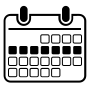
\includegraphics[width=\linewidth]{figs/noun_week_247256.svg}
\end{sbspanel}%
\end{sidebyside}%
\begin{example}{Days of the Week.}{x:example:eg-cong-week}%
Modulo 7, the numbers 26 and 47 are congruent because \(7 \mid (26-47)\). This means 26 and 47 are `equivalent' under this particular relation.%
\par
One way to see this is the fact that if today were Sunday, then 26 days from today it will be Friday, and 47 days from today is also a Friday. Abstracting only the property we care about (remainder when divided by 7) allows us to generate conclusions like this without having to manually count 47 days forward.%
\par
As another example, if today were Sunday, then we can confidently claim that 2020 days from today, it will be Thursday. This is because \(2020 \equiv 4 \Mod{7}\), and four days after Sunday is Thursday. (We've effectively removed as many 7's as possible to reduce the calculation.)%
\end{example}
\begin{inlineexercise}{New Relationship.}{x:exercise:eg-cong-week-2}%
Today, two of your friends bought each other matching couple shirts to celebrate being in a relationship for 100 days. If today is Wednesday, what day did their relationship begin?%
\end{inlineexercise}
\begin{definition}{Congruence Class.}{x:definition:def-congruence-class}%
The equivalence classes of congruence modulo \(n\) are called \terminology{congruence classes} or \terminology{remainder classes}, and they are the sets%
\begin{equation*}
\mathbb{Z}_n = \{[0],[1],[2],\ldots,[n-1]\}\text{,}
\end{equation*}
corresponding to the possible remainders when dividing by \(n\). \label{g:notation:id444993}%
\end{definition}
\begin{example}{Modulo 5.}{x:example:eg-cong-mod5}%
Modulo 5, the congruence classes are%
\begin{align*}
[0] \amp = \{\ldots,-10,-5,0,5,10,\ldots\}\\
[1] \amp = \{\ldots,-9,-4,1,6,11,\ldots\}\\
[2] \amp = \{\ldots,-8,-3,2,7,12,\ldots\}\\
[3] \amp = \{\ldots,-7,-2,3,8,13,\ldots\}\\
[4] \amp = \{\ldots,-6,-1,4,9,14,\ldots\}
\end{align*}
%
\end{example}
Observe that if two numbers \(a\) and \(b\) are congruent modulo \(n\), then their difference \(a-b\) is congruent to 0 modulo \(n\). This is because \(a\) and \(b\) are essentially \emph{the same} when working modulo \(n\) (the remainder is all that matters), so subtracting them will give `0' in that framework.%
\par
We can perform addition and multiplication modulo \textdollar{}n\textdollar{} as well.%
\begin{proposition}{Modular Arithmetic.}{}{x:proposition:prop-cong-modular-arithmetic}%
Let \(n\) be a natural number, and \(a, b, r, s\) integers such that \(a \equiv r \Mod{n}\) and \(b \equiv s \Mod{n}\). Then:%
\begin{enumerate}[label=(\alph*)]
\item{}\(a + b \equiv r + s \Mod{n}\).%
\item{}\(ab \equiv rs \Mod{n}\).%
\item{}\(a^k \equiv r^k \Mod{n}\) for any \(k \in \mathbb{N}\).%
\end{enumerate}
%
\end{proposition}
\begin{inlineexercise}{prove Proposition~{\xreffont\ref*{x:proposition:prop-cong-modular-arithmetic}}.}{x:exercise:ex-cong-prove-modular-arithmetic}%
Prove \hyperref[x:proposition:prop-cong-modular-arithmetic]{Proposition~{\xreffont\ref{x:proposition:prop-cong-modular-arithmetic}}}.%
\end{inlineexercise}
Importantly, \hyperref[x:proposition:prop-cong-modular-arithmetic]{Proposition~{\xreffont\ref{x:proposition:prop-cong-modular-arithmetic}}} implies that in any congruence, we can replace any number with another number it is congruent to, and obtain an equivalent statement.%
\begin{example}{Substituting Congruent Numbers.}{x:example:eg-cong-modular-arithmetic}%
Suppose we wanted to compute the remainder when 4133 is divided by 4. We first write \(4133 = 4000 + 100 + 30 + 3\), so that%
\begin{equation*}
4000 + 100 + 30 + 3 \equiv 0 + 0 + 2 + 3 \Mod{4} \equiv 1 \Mod{4}\text{.}
\end{equation*}
Hence the remainder when 4133 is divided by 4 is 1.%
\end{example}
\begin{definition}{The Modulo Operation.}{x:definition:def-cong-modulo}%
Given two integers \(a\) and \(m\), with \(m \ne 0\), the \terminology{modulo operation} denoted by%
\begin{equation*}
a \mmod{m}\text{,}
\end{equation*}
read as \emph{\(a\) modulo \(m\)}, is the remainder obtained from \hyperref[x:theorem:thm-division-algorithm]{Theorem~{\xreffont\ref{x:theorem:thm-division-algorithm}}} when \(a\) is divided by \(m\). \label{g:notation:id445197}%
\end{definition}
\begin{inlineexercise}{Compute Remainders.}{x:exercise:ex-cong-compute-remainder}%
Compute the following:%
\begin{enumerate}[label=(\alph*)]
\item{}\(\displaystyle 2139138 \mmod 9\)%
\item{}\(\displaystyle 2^{1000} \mmod 7\)%
\item{}\(\displaystyle 10! \mmod 17\)%
\end{enumerate}
%
\end{inlineexercise}
While \hyperref[x:proposition:prop-cong-modular-arithmetic]{Proposition~{\xreffont\ref{x:proposition:prop-cong-modular-arithmetic}}} allows us to perform addition, subtraction and multiplication, when we try dividing we find that we run into some issues.%
\begin{example}{Division is not as Nice.}{x:example:eg-cong-dividing-doesnt-work}%
We know that%
\begin{equation*}
39 \equiv 123 \Mod{12}\text{.}
\end{equation*}
If we divide both sides by 3, we would get%
\begin{equation*}
13 \equiv 41 \Mod{12}\text{,}
\end{equation*}
which is \emph{false}. However \(13 \equiv 41 \Mod{4}\) is true.%
\end{example}
\begin{proposition}{Dividing both sides of a Congruence.}{}{x:proposition:prop-cong-division}%
Let \(n \in \mathbb{N}\) and \(a,b,d \in \mathbb{Z}\). If \(ad \equiv bd \Mod{n}\), then%
\begin{equation*}
a \equiv b \Mod{\dfrac{n}{\gcd(d,n)}}\text{.}
\end{equation*}
%
\par
If \(d\) and \(n\) are relatively prime, then \(ad \equiv bd \Mod{n}\) implies%
\begin{equation*}
a \equiv b \Mod{n}\text{.}
\end{equation*}
%
\end{proposition}
\begin{proof}{}{g:proof:id445306}
Suppose that \(ad \equiv bd \Mod{n}\). This means \(ad = bd + kn\) for some \(k \in \mathbb{Z}\).%
\par
Since \(\gcd(d,n)\) divides both \(d\) and \(n\), we can divide through to get%
\begin{equation*}
a\cdot \dfrac{d}{\gcd(d,n)} = b\cdot \dfrac{d}{\gcd(d,n)} + k \cdot\dfrac{n}{\gcd(d,n)}\text{.}
\end{equation*}
%
\par
This is equivalent to%
\begin{equation*}
\dfrac{n}{\gcd(d,n)} \ \Biggl\vert \ (a-b)\left(\dfrac{d}{\gcd(d,n)}\right)\text{.}
\end{equation*}
Since \(\gcd\left(\dfrac{d}{\gcd(d,n)},\dfrac{n}{\gcd(d,n)}\right) = 1\), we can apply the result of \hyperref[x:exercise:ex-review-bezout-euclid]{Checkpoint~{\xreffont\ref{x:exercise:ex-review-bezout-euclid}}} to obtain%
\begin{equation*}
\dfrac{n}{\gcd(d,n)} \ \Biggl\vert \ (a-b)\text{,}
\end{equation*}
or that \(a \equiv b \Mod{\dfrac{n}{\gcd(d,n)}}\), as desired.%
\par
If \(\gcd(d,n) = 1\), the statement reduces to \(a \equiv b \Mod{n}\).%
\end{proof}
\begin{inlineexercise}{Justify It.}{x:exercise:ex-cong-division-explain}%
Explain why%
\begin{equation*}
\gcd\left(\dfrac{d}{\gcd(d,n)},\dfrac{n}{\gcd(d,n)}\right) = 1
\end{equation*}
in the proof of \hyperref[x:proposition:prop-cong-division]{Proposition~{\xreffont\ref{x:proposition:prop-cong-division}}}.%
\par\smallskip%
\noindent\textbf{\blocktitlefont Hint}.\hypertarget{g:hint:id445384}{}\quad{}Contradiction.%
\end{inlineexercise}
The second statement of \hyperref[x:proposition:prop-cong-division]{Proposition~{\xreffont\ref{x:proposition:prop-cong-division}}} is also called the \alert{cancellation law}, since it gives a condition under which one can divide both sides of a congruence by a number.%
%
%
\typeout{************************************************}
\typeout{Solutions 4.2.1 Solutions to Selected Checkpoints}
\typeout{************************************************}
%
\begin{solutions-subsection}{Solutions to Selected Checkpoints}{}{Solutions to Selected Checkpoints}{}{}{g:solutions:id445382}
\end{solutions-subsection}
\end{sectionptx}
%
%
\typeout{************************************************}
\typeout{Section 4.3 Solving Congruences}
\typeout{************************************************}
%
\begin{sectionptx}{Solving Congruences}{}{Solving Congruences}{}{}{x:section:sec-congruence-solving}
\begin{objectives}{Objectives}{g:objectives:id445377}
%
\begin{itemize}[label=\textbullet]
\item{}Determine if an integer has a multiplicative inverse, and find it if it exists.%
\item{}Solve linear congruences by using properties of congruence and\slash{}or finding the multiplicative inverse.%
\end{itemize}
\end{objectives}
When we are asked to \emph{solve for \(x\)} in an equation like \(2x^2 + 4 = 36\), we know that we need to look for all values of \(x\) that satisfy that equation (\(x = \pm 4\)). What if we are asked to solve for \(x\) given a congruence?%
\begin{example}{Solving for \(x\).}{x:example:eg-cong-solve-congruence}%
Solve for \(x\) in the congruence \(2x \equiv 4 \Mod{9}\).%
\par
Before looking at the solution, try it yourself first! What value(s) of \(x\) will satisfy the congruence?%
\par\smallskip%
\noindent\textbf{\blocktitlefont Solution}.\hypertarget{g:solution:id443234}{}\quad{}We need to find all values of \(x\) so that \(9 \mid (2x - 4)\), or \(9 \mid 2(x-2)\).%
\par
Since \(\gcd(2,9) = 1\), by \hyperref[x:exercise:ex-review-bezout-euclid]{Checkpoint~{\xreffont\ref{x:exercise:ex-review-bezout-euclid}}} we have \(9 \mid (x-2)\), which means \(x \equiv 2 \Mod{9}\).%
\par
Note that this is no different from applying \hyperref[x:proposition:prop-cong-division]{Proposition~{\xreffont\ref{x:proposition:prop-cong-division}}} directly: since \(\gcd(2,9) = 1\), we can safely divide both sides by 2 to obtain \(x \equiv 2 \Mod{9}\).%
\par
This means that the congruence class \([2]\) is the solution to \(2x \equiv 4 \Mod{9}\), or that all integers in \(\{\ldots,-16,-7,2,11,\ldots\}\) satisfy the congruence.%
\end{example}
The final answer in the above example is typical of solutions to congruences: since we are working modulo \(n\), answers will be congruence classes from \(\{[0],[1],\ldots,[n-1]\}\). Hence when asked to \emph{solve for \(x\)} given a congruence, you should express your answer as a congruence class (\([2]\)), or as a statement of congruence like \(x \equiv 2 \Mod{9}\), which makes the modulus explicit.%
\begin{example}{Solve for \(x\).}{x:example:eg-cong-solve-congruence-express}%
Solve the congruence%
\begin{equation*}
2x \equiv 6 \Mod{10}\text{,}
\end{equation*}
and express your answer using congruence classes of the original modulus.%
\par\smallskip%
\noindent\textbf{\blocktitlefont Solution}.\hypertarget{g:solution:id443298}{}\quad{}We can apply \hyperref[x:proposition:prop-cong-division]{Proposition~{\xreffont\ref{x:proposition:prop-cong-division}}} here to divide through by 2, and we get%
\begin{equation*}
x \equiv 3 \Mod{5}\text{.}
\end{equation*}
Modulo 10, this is the same as%
\begin{equation*}
x \equiv 3 \Mod{10} \text{ and } x \equiv 8 \Mod{10}\text{.}
\end{equation*}
So the original congruence has two solutions in \(\{[0],[1],\ldots,[9]\}\), namely \([3]\) and \([8]\).%
\end{example}
\begin{inlineexercise}{Solve Each Congruence.}{x:exercise:ex-cong-solve-for-x}%
Solve each congruence for \(x\), paying special attention to your usage of \hyperref[x:proposition:prop-cong-division]{Proposition~{\xreffont\ref{x:proposition:prop-cong-division}}}.%
\begin{enumerate}[label=(\alph*)]
\item{}\(\displaystyle 3x \equiv 9 \Mod{10}\)%
\item{}\(\displaystyle 5x + 2 \equiv 27 \Mod{15}\)%
\item{}\(\displaystyle -11x - 3 \equiv 30 \Mod{7}\)%
\end{enumerate}
%
\end{inlineexercise}
\begin{inlineexercise}{Solve Another One.}{x:exercise:ex-cong-trial-error}%
\hyperref[x:proposition:prop-cong-division]{Proposition~{\xreffont\ref{x:proposition:prop-cong-division}}} cannot be used to solve the congruence%
\begin{equation*}
2x \equiv 3 \Mod{7}
\end{equation*}
since we cannot divide both sides by 2.%
\par
Solve the congruence by trial-and-error.%
\par\smallskip%
\noindent\textbf{\blocktitlefont Hint}.\hypertarget{g:hint:id443380}{}\quad{}There are only 7 congruence classes to check, since we are working modulo 7.%
\end{inlineexercise}
We've seen that dividing both sides by a constant is not always possible. Recall instead that in the real numbers, division by a nonzero number \(x\) is the same as multiplication by its reciprocal \(\frac{1}{x}\). The number \(\frac{1}{x}\) is sometimes called the \emph{inverse} of \(x\) since they `cancel' each other out when multplied together.%
\par
We define a similar concept for modular arithmetic.%
\begin{definition}{Multiplicative Inverse.}{x:definition:def-multiplicative-inverse}%
Given natural numbers \(a, m\) such that \(\gcd(a,m) = 1\), the number \(b\) is called a \terminology{multiplicative inverse} of \(a\) modulo \(m\) if%
\begin{equation*}
ab \equiv 1 \Mod{m}\text{.}
\end{equation*}
%
\par
We can denote this inverse as \(a^{-1} = b\), or by \(a^{-1} \Mod{m}\) to make the modulus explicit.%
\end{definition}
In \hyperref[x:definition:def-multiplicative-inverse]{Definition~{\xreffont\ref{x:definition:def-multiplicative-inverse}}} we are really saying that any number in \([b]\) is a multiplicative inverse of \(a\) modulo \(m\), though we will usually be interested in finding that specific inverse that is also in the set \(\{0,1,\ldots,m-1\}\). This can now be used when solving congruences of the form%
\begin{equation*}
ax \equiv b \Mod{n}
\end{equation*}
where \(a \nmid b\). Instead of dividing both sides by \(a\) (which can't always be done), we multiply both sides by the inverse of \(a\).%
\begin{inlineexercise}{Checkpoint~{\xreffont\ref*{x:exercise:ex-cong-trial-error}} Again.}{x:exercise:ex-cong-multiplicative-inverse}%
Show that modulo 7, any number in \([4]\) is a multiplicative inverse of 2. Then use this fact to solve the congruence%
\begin{equation*}
2x \equiv 3 \Mod{7}
\end{equation*}
from \hyperref[x:exercise:ex-cong-trial-error]{Checkpoint~{\xreffont\ref{x:exercise:ex-cong-trial-error}}}.%
\end{inlineexercise}
\begin{inlineexercise}{The Multiplicative Inverse is Unique.}{x:exercise:ex-cong-prove-inverse-unique}%
Given \(a, m \in \mathbb{N}\) such that \(\gcd(a,m) = 1\), prove that the multiplicative inverse of \(a\) modulo \(m\) is unique (up to congruence class).%
\par\smallskip%
\noindent\textbf{\blocktitlefont Hint}.\hypertarget{g:hint:id443587}{}\quad{}Assume that \(c\) and \(d\) are both multiplicative inverses of \(a\) modulo \(m\). Show that \(c \equiv d \Mod{m}\).%
\end{inlineexercise}
\begin{inlineexercise}{Uniqueness of Solutions.}{x:exercise:ex-cong-rel-prime-unique}%
Use the previous exercise to argue that%
\begin{equation*}
ax \equiv b \Mod{m}
\end{equation*}
has a unique solution (up to congruence class) if \(\gcd(a,m) = 1\).%
\par
Does the converse hold? That is, if we know that%
\begin{equation*}
ax \equiv b \Mod{m}
\end{equation*}
has a unique solution, can we conclude that \(\gcd(a,m) = 1\)?%
\end{inlineexercise}
\begin{inlineexercise}{Solve These Congruences.}{x:exercise:ex-cong-solve-congruences}%
Solve the congruences:%
\begin{enumerate}[label=(\alph*)]
\item{}\(\displaystyle 5x - 7 \equiv 9 \Mod{11}\)%
\item{}\(\displaystyle 3 - 2x \equiv 3 - 5x \Mod{7}\)%
\item{}\(\displaystyle 21x + 35 \equiv 9 \Mod{19}\)%
\end{enumerate}
%
\end{inlineexercise}
\begin{inlineexercise}{How Many Solutions?}{x:exercise:ex-cong-how-many-solutions}%
Since \(\gcd(6,16) \gt 1\), the number 6 has no multiplicative inverse modulo 16. Solve the congruences%
\begin{equation*}
6x \equiv 3 \Mod{16}
\end{equation*}
and%
\begin{equation*}
6x \equiv 4 \Mod{16}\text{.}
\end{equation*}
How many solutions do you get for each one (modulo 16)?%
\end{inlineexercise}
%
%
\typeout{************************************************}
\typeout{Solutions 4.3.1 Solutions to Selected Checkpoints}
\typeout{************************************************}
%
\begin{solutions-subsection}{Solutions to Selected Checkpoints}{}{Solutions to Selected Checkpoints}{}{}{g:solutions:id443978}
\end{solutions-subsection}
\end{sectionptx}
%
%
\typeout{************************************************}
\typeout{Section 4.4 Euler's Theorem}
\typeout{************************************************}
%
\begin{sectionptx}{Euler's Theorem}{}{Euler's Theorem}{}{}{x:section:sec-euler}
\begin{objectives}{Objectives}{g:objectives:id444039}
%
\begin{itemize}[label=\textbullet]
\item{}Define Euler's totient function \(\phi(n)\), compute its values for small \(n\), and prove general statements about \(\phi(n)\).%
\item{}State and apply Euler's Theorem and Fermat's Little Theorem to solve congruences and prove other results.%
\item{}Apply Fermat's Little Theorem to primality testing.%
\end{itemize}
\end{objectives}
First, let's restate the definition of Euler's totient function (introduced in \hyperref[x:exploration:expl-pie-euler-totient]{Exploration~{\xreffont\ref{x:exploration:expl-pie-euler-totient}}}).%
\begin{definition}{Euler's Totient Function.}{x:definition:def-euler-totient}%
\terminology{Euler's totient function} (or \terminology{Euler's phi-function}) is the function \(\phi: \mathbb{N} \rightarrow \mathbb{N}\) defined by%
\begin{equation*}
\phi(m) = \bigl|\{k \in \mathbb{N} : 1 \leq k \leq m, \gcd(k,m) = 1\}\bigr|\text{.}
\end{equation*}
%
\label{g:notation:id221341}%
\end{definition}
\begin{example}{\(\phi(1)\) and \(\phi(8)\).}{x:example:eg-cong-totient}%
We have \(\phi(1) = 1\) since \(1\) is the only integer in \(\{1\}\) relatively prime with 1.%
\par
Also \(\phi(8) = 4\), since there are four numbers in the set \(\{1,2,\ldots,8\}\) relatively prime with 8: they are 1, 3, 5, and 7.%
\end{example}
\begin{inlineexercise}{\(\phi(n)\) for small \(n\).}{x:exercise:ex-cong-totient}%
The table below lists values of \(\phi(m)\) for small values of \(m\). Complete the table for \(m = 11, 12, \ldots, 20\).%
\begin{tableptx}{\textbf{}}{x:table:table-euler-totient-values}{}%
\centering
{\tabularfont%
\begin{tabular}{ccc}
\(m\)&integers \(1 \leq k \leq m\)&\(\phi(m)\)\tabularnewline[0pt]
&such that \(\gcd(k,m)=1\)&\tabularnewline\hrulemedium
1&1&1\tabularnewline[0pt]
2&1&1\tabularnewline[0pt]
3&1, 2&2\tabularnewline[0pt]
4&1, 3&2\tabularnewline[0pt]
5&1, 2, 3, 4&4\tabularnewline\hrulemedium
6&1, 5&2\tabularnewline[0pt]
7&1, 2, 3, 4, 5, 6&6\tabularnewline[0pt]
8&1, 3, 5, 7&4\tabularnewline[0pt]
9&1, 2, 4, 5, 7, 8&6\tabularnewline[0pt]
10&1, 3, 7, 9&4\tabularnewline\hrulemedium
11&&\tabularnewline[0pt]
12&&\tabularnewline[0pt]
13&&\tabularnewline[0pt]
14&&\tabularnewline[0pt]
15&&\tabularnewline\hrulemedium
16&&\tabularnewline[0pt]
17&&\tabularnewline[0pt]
18&&\tabularnewline[0pt]
19&&\tabularnewline[0pt]
20&&\tabularnewline\hrulemedium
\end{tabular}
}%
\end{tableptx}%
\end{inlineexercise}
If \(p\) is prime, then by definition all integers from \(1\) to \(p-1\) are relatively prime with \(p\). This implies the following result:%
\begin{proposition}{\(\phi(p)\).}{}{x:proposition:prop-euler-totient-prime}%
If \(p\) is prime, then \(\phi(p) = p-1\).%
\end{proposition}
\begin{inlineexercise}{Converse of Proposition~{\xreffont\ref*{x:proposition:prop-euler-totient-prime}}.}{x:exercise:ex-cong-euler-totient-prime-converse}%
Is the converse of the above statement true? That is, if \(m \gt 2\) is an integer such that \(\phi(m) = m-1\), does it necessarily follow that \(m\) is prime?%
\par
Justify your answer.%
\end{inlineexercise}
\begin{inlineexercise}{\(\phi(p^k)\).}{x:exercise:ex-cong-euler-totient-prime-power}%
If \(p\) is prime and \(k \in \mathbb{N}\), prove that \(\phi(p^k) = p^k - p^{k-1}\).%
\end{inlineexercise}
\begin{inlineexercise}{\(\phi(pq)\).}{x:exercise:ex-cong-euler-totient-prime-product}%
If \(p\) and \(q\) are prime, prove that \(\phi(pq) = (p-1)(q-1)\).%
\par\smallskip%
\noindent\textbf{\blocktitlefont Hint}.\hypertarget{g:hint:id453538}{}\quad{}\hyperref[x:theorem:thm-pie]{Theorem~{\xreffont\ref{x:theorem:thm-pie}}}%
\end{inlineexercise}
Now we can state Euler's Theorem then prove Fermat's Little Theorem, which is a special case.%
\begin{theorem}{Euler's Theorem.}{}{x:theorem:thm-euler}%
If \(a, m \in \mathbb{N}\) with \(\gcd(a,m) = 1\), then%
\begin{equation*}
a^{\phi(m)} \equiv 1 \Mod{m}\text{.}
\end{equation*}
%
\end{theorem}
\begin{theorem}{Fermat's Little Theorem (FLT).}{}{x:theorem:thm-flt}%
If \(a \in \mathbb{N}\) and \(p\) is prime such that \(p \nmid a\), then%
\begin{equation*}
a^{p-1} \equiv 1 \Mod{p}\text{.}
\end{equation*}
%
\end{theorem}
\begin{proof}{}{g:proof:id453619}
If \(p\) is prime with \(p \nmid a\), we have \(\gcd(a,p) = 1\). So we can use \hyperref[x:theorem:thm-euler]{Theorem~{\xreffont\ref{x:theorem:thm-euler}}} on \(a\) and \(m = p\). Since \(\phi(p) = p-1\) by \hyperref[x:proposition:prop-euler-totient-prime]{Proposition~{\xreffont\ref{x:proposition:prop-euler-totient-prime}}}, the result follows.%
\end{proof}
Although \hyperref[x:theorem:thm-flt]{Theorem~{\xreffont\ref{x:theorem:thm-flt}}} is a special case of \hyperref[x:theorem:thm-euler]{Theorem~{\xreffont\ref{x:theorem:thm-euler}}}, it was \hyperref[x:theorem:thm-flt]{Theorem~{\xreffont\ref{x:theorem:thm-flt}}} that was actually proven first\textemdash{}in 1736, also by Euler \hyperlink{x:biblio:bib-euler-54}{[{\xreffont 1}]}. Only in 1763 did Euler publish the generalization that is Euler's Theorem \hyperlink{x:biblio:bib-euler-271}{[{\xreffont 2}]}.%
\begin{example}{Example of Theorem~{\xreffont\ref*{x:theorem:thm-euler}}.}{x:example:eg-cong-euler-apply}%
Take \(m = 8\) and \(a = 7\) so that \(\gcd(a,m) = 1\). By \hyperref[x:theorem:thm-euler]{Theorem~{\xreffont\ref{x:theorem:thm-euler}}} we have%
\begin{equation*}
7^{\phi(8)} \equiv 1 \Mod{8} \Rightarrow 7^4 \equiv 1 \Mod{8}\text{.}
\end{equation*}
%
\end{example}
\begin{example}{Compute the Remainder.}{x:example:eg-cong-euler-remainder}%
Compute \(3^{2020} \mmod 113\).%
\par\smallskip%
\noindent\textbf{\blocktitlefont Solution}.\hypertarget{g:solution:id453693}{}\quad{}Since \(\gcd(3,113) = 1\), we can apply \hyperref[x:theorem:thm-euler]{Theorem~{\xreffont\ref{x:theorem:thm-euler}}}. In fact, 113 is prime, so \hyperref[x:theorem:thm-flt]{Theorem~{\xreffont\ref{x:theorem:thm-flt}}} applies here, so we know that%
\begin{equation*}
3^{112} \equiv 1 \Mod{13}\text{.}
\end{equation*}
Using the \hyperref[x:theorem:thm-division-algorithm]{Theorem~{\xreffont\ref{x:theorem:thm-division-algorithm}}} on 2020 we get \(2019 = 18\cdot 112 + 4\). Hence%
\begin{equation*}
3^{2020} \equiv (3^{112})^{18} \cdot 3^4 \Mod{113} \equiv 81 \Mod{113}\text{.}
\end{equation*}
So \(3^{2020} \mmod 113 = 81\).%
\end{example}
\begin{inlineexercise}{Compute the Remainder.}{x:exercise:ex-cong-euler-remainder}%
Compute \(6^{6777} \mmod 667\).%
\par\smallskip%
\noindent\textbf{\blocktitlefont Hint}.\hypertarget{g:hint:id453714}{}\quad{}\(667 = 23 \times 29.\)%
\end{inlineexercise}
The idea behind the proof of \hyperref[x:theorem:thm-euler]{Theorem~{\xreffont\ref{x:theorem:thm-euler}}} is that for \(a,m \in \mathbb{N}\) relatively prime, multiplying each element of the set%
\begin{equation*}
S = \{y \in \{1,2,\ldots,m\} : \gcd(y,m) = 1\}
\end{equation*}
by \(a\) induces a permutation of the set modulo \(m\). We give first an example with numbers.%
\begin{example}{Why Theorem~{\xreffont\ref*{x:theorem:thm-euler}} holds, for \(a = 4\) and \(m = 9\).}{x:example:eg-cong-euler-proof-example}%
Let \(a = 4\) and \(m = 9\). Then \(\phi(9) = 6\), since the integers \(S = \{1,2,4,5,7,8\}\) are relatively prime with \(9\).%
\par
Multiplying each number in \(S\) by 4 and reducing modulo 9, we have%
\begin{sidebyside}{1}{0.125}{0.125}{0}%
\begin{sbspanel}{0.75}%
{\centering%
{\tabularfont%
\begin{tabular}{cccccccc}
\multicolumn{1}{r}{\(S = \)}&\(\{\)1&2&4&5&7&8\(\}\)&\multicolumn{1}{l}{}\tabularnewline[0pt]
\multicolumn{1}{r}{}&\(\downarrow\)&\(\downarrow\)&\(\downarrow\)&\(\downarrow\)&\(\downarrow\)&\(\downarrow\)&\multicolumn{1}{l}{(multiply by \(a = 4\))}\tabularnewline[0pt]
\multicolumn{1}{r}{}&4&8&16&20&28&32&\multicolumn{1}{l}{}\tabularnewline[0pt]
\multicolumn{1}{r}{}&\(\downarrow\)&\(\downarrow\)&\(\downarrow\)&\(\downarrow\)&\(\downarrow\)&\(\downarrow\)&\multicolumn{1}{l}{(reduce modulo 9)}\tabularnewline[0pt]
\multicolumn{1}{r}{}&\(\{\)4&8&7&2&1&5\(\}\)&\multicolumn{1}{l}{\(\rightarrow\) same as \(S\)!}
\end{tabular}
}%
\par}
\end{sbspanel}%
\end{sidebyside}%
\par
What this means is that \(S\) and \(\{4y : y \in S\}\) contain the same numbers modulo 9; so when we take the product of all elements in these sets, the results must be congruent modulo 9 as well:%
\begin{equation*}
(4\cdot 1)(4\cdot 2)(4\cdot 4)(4 \cdot 5)(4\cdot 7)(4\cdot 8) \equiv (1)(2)(4)(5)(7)(8)\Mod{9}\text{.}
\end{equation*}
%
\par
Since each element of \(S\) is relatively prime with 9, we can apply \hyperref[x:proposition:prop-cong-division]{Proposition~{\xreffont\ref{x:proposition:prop-cong-division}}} to cancel each term, and we are left with%
\begin{equation*}
(4)(4)(4)(4)(4)(4) \equiv 1 \Mod{9} \Rightarrow 4^{\phi(9)} \equiv 1 \Mod{9}
\end{equation*}
since \(\phi(9) = 6 = |S|\).%
\end{example}
\begin{inlineexercise}{Repeat the Argument.}{x:exercise:ex-cong-euler-proof-example-again}%
Replicate the idea in \hyperref[x:example:eg-cong-euler-proof-example]{Example~{\xreffont\ref{x:example:eg-cong-euler-proof-example}}} to show that \(7^{\phi(15)} \equiv 1 \Mod{15}\).%
\end{inlineexercise}
Finally, we present the proof of \hyperref[x:theorem:thm-euler]{Theorem~{\xreffont\ref{x:theorem:thm-euler}}}.\alert{Proof of Euler's Theorem}%
\par
Let \(a,m \in \mathbb{N}\) such that \(\gcd(a,m) = 1\).%
\par
First define the set%
\begin{equation*}
S = \{y : 1 \leq y \leq m, \gcd(y,m) = 1\}
\end{equation*}
to be the set of natural numbers smaller than \(m\) and relatively prime with \(m\). We know that there are exactly \(\phi(m)\) elements in the set \(S\), so we can label them as \(S = \{b_1,b_2,\ldots,b_{\phi(m)}\}\), where \(\gcd(b_i,m) = 1\) for \(i = 1,2,\ldots,\phi(m)\).%
\par
Since we have \(\gcd(b_i,m) = 1\) and \(\gcd(a,m) = 1\), we must also have%
\begin{equation*}
\gcd(ab_i, m) = 1 \text{ for any } i = 1,2,\ldots,\phi(m)\text{.}
\end{equation*}
We invoke \hyperref[x:theorem:thm-division-algorithm]{Theorem~{\xreffont\ref{x:theorem:thm-division-algorithm}}} now to write \(ab_i\) as%
\begin{equation*}
ab_i = qm + r \text{ for some } 0 \leq r \lt m,
\end{equation*}
which implies that \(ab_i \equiv r \Mod{m}\).%
\par
Combining with the fact that \(\gcd(ab_i,m) = 1\), this implies that \(\gcd(r,m) = 1\), so \(r\) is a natural number smaller than \(m\) and relatively prime with \(m\).%
\par
In other words, \(r\) is in the set \(S\), and we can write \(r = b_j\) for some \(1 \leq j \leq \phi(m)\). This means for each \(1 \leq i \leq \phi(m)\), we have \(ab_i \equiv b_j \Mod{m}\) for some \(1 \leq j \leq \phi(m)\).%
\par
Furthermore, none of the \(b_j\)'s are repeated, because no two \(ab_i\) terms are equivalent modulo \(m\). (Otherwise, \(ab_{i_1} \equiv ab_{i_2} \Mod{m} \Rightarrow b_{i_1} \equiv b_{i_2} \Mod{m}\) by \hyperref[x:proposition:prop-cong-division]{Proposition~{\xreffont\ref{x:proposition:prop-cong-division}}}, which is a contradiction as the \(b_i\)'s are all distinct and smaller than \(m\).)%
\par
Hence, each integer \(ab_i\) is congruent modulo \(m\) to distinct elements in \(S\):%
\begin{align*}
ab_1 \amp \equiv b_{j_1} \Mod{m}\\
ab_2 \amp \equiv b_{j_2} \Mod{m}\\
\vdots \amp\\
ab_{\phi(m)} \amp \equiv b_{j_{\phi(m)}} \Mod{m}
\end{align*}
Multiplying all the congruences together gives another congruence, where the right-hand-side is just%
\begin{equation*}
\displaystyle\prod_{k=1}^{\phi(m)} b_{j_k} = \displaystyle\prod_{i=1}^{\phi(m)} b_i
\end{equation*}
since each element of \(S\) appears exactly once. Hence,%
\begin{equation*}
\prod_{i=1}^{\phi(m)} ab_i \equiv \prod_{i=1}^{\phi(m)} b_i \Mod{m} \Rightarrow a^{\phi(m)} \equiv 1 \Mod{m}
\end{equation*}
by an application of \hyperref[x:proposition:prop-cong-division]{Proposition~{\xreffont\ref{x:proposition:prop-cong-division}}}.%
\begin{exploration}{Primality Testing.}{x:exploration:expl-primality-testing}%
\hyperref[x:theorem:thm-flt]{Theorem~{\xreffont\ref{x:theorem:thm-flt}}} asserts that \alert{if} \(p\) is prime and \(\gcd(a,p)=1\), \alert{then} \(a^{p-1} \equiv 1 \Mod{p}\).%
\begin{enumerate}[font=\bfseries,label=(\alph*),ref=\alph*]
\item{}Note that the converse of this statement is not true in general: Even if \(\gcd(a,m) = 1\) and \(a^{m-1} \equiv 1 \Mod{m}\), we would not be able to conclude that \(m\) is prime.%
\par
Can you give examples of pairs \(a, m\) such that \(\gcd(a,m) = 1\) and \(a^{m-1} \equiv 1 \Mod{m}\) are both true, but \(m\) is not prime.%
\item{}Complete the contrapositive of \hyperref[x:theorem:thm-flt]{Theorem~{\xreffont\ref{x:theorem:thm-flt}}}:%
\begin{sidebyside}{1}{0.1}{0.1}{0}%
\begin{sbspanel}{0.8}%
\alert{If} \(a,m \in \mathbb{N}\), \(\gcd(a,m) = 1\), and \(a^{m-1} \not\equiv 1 \Mod{m}\), \alert{then} \fillin{11.3636363636364}.%
\end{sbspanel}%
\end{sidebyside}%
\item{}Show that 91 is not prime by using part (b) with \(a = 2\).%
\end{enumerate}
\end{exploration}
\end{sectionptx}
%
%
\typeout{************************************************}
\typeout{Section 4.5 The Chinese Remainder Theorem}
\typeout{************************************************}
%
\begin{sectionptx}{The Chinese Remainder Theorem}{}{The Chinese Remainder Theorem}{}{}{x:section:sec-chinese-remainder}
\begin{objectives}{Objectives}{g:objectives:id454338}
%
\begin{itemize}[label=\textbullet]
\item{}State the Chinese Remainder Theorem and use it to solve systems of congruences and related problems.%
\end{itemize}
\end{objectives}
The Chinese Remainder Theorem is a result in number theory about solving simultaneous systems of several linear congruences. In this section we explore its origins and give methods to solve these systems.%
\begin{exploration}{Sun Zi's Problem.}{x:exploration:expl-sunzi}%
Sun Zi (\text{\textit{孙子}}) was a Chinese mathematician who in his text \href{https://en.wikipedia.org/wiki/Sunzi_Suanjing}{\pubtitle{Sunzi Suanjing}}\text{\textit{《孙子算经》}} (3rd to 5th century AD) is said to have written the earliest known reference to systems of linear congruences. In it he writes:%
\begin{quote}%
`\text{\textit{今有物,不知其数。三、三数之,剩二;五、五数之,剩三;七、七数之,剩二。问物几何?}}'%
\nopagebreak\par%
\hfill\textemdash{}{\setlength{\tabcolsep}{0pt}\begin{tabular}[t]{l@{}}
\text{\textit{孙子。《孙子算经》。}}
\end{tabular}}\\\par
\end{quote}
\begin{quote}%
`A number is repeatedly divided by 3, the remainder is 2; divided by 5, the remainder is 3; and by 7, the remainder is 2. What will the number be?'%
\nopagebreak\par%
\hfill\textemdash{}{\setlength{\tabcolsep}{0pt}\begin{tabular}[t]{l@{}}
Sun Zi, \pubtitle{Sunzi Suanjing}, Vol. 3, Problem 26 (as cited in \hyperlink{x:biblio:bib-kangsheng-1988}{[{\xreffont 4}]})
\end{tabular}}\\\par
\end{quote}
We follow Sun Zi's method of solving this system.%
\begin{enumerate}[font=\bfseries,label=(\alph*),ref=\alph*]
\item{}The first condition in Sun Zi's problem can be written as%
\begin{equation*}
x \equiv 2 \Mod{3}\text{.}
\end{equation*}
Write all three conditions as a system of linear congruences.%
\textbf{\blocktitlefont Answer}.\hypertarget{g:answer:id454435}{}\quad{}%
\begin{equation*}
\begin{cases} x \equiv 2 \Mod{3} \\ x \equiv 3 \Mod{5} \\ x \equiv 2 \Mod{7} \end{cases}
\end{equation*}
%
\item{}Since the integers 3, 5, and 7 are pairwise relatively prime, then \(35^{-1} \Mod{3}\) exists. Compute this quantity.%
\par
Similarly, compute \(21^{-1} \Mod{5}\) and \(15^{-1} \Mod{7}\).%
\item{}Explain why each of the following congruences hold:%
\begin{equation*}
\begin{cases} 2 \cdot 35^{-1} \cdot 35 \equiv 2 \Mod{3} \\ 3 \cdot 21^{-1} \cdot 21 \equiv 3 \Mod{5} \\ 2 \cdot 15^{-1} \cdot 15 \equiv 2 \Mod{7} \end{cases}\text{.}
\end{equation*}
%
\item{}Explain why we can conclude that%
\begin{equation*}
x \equiv 2 \cdot 35^{-1} \cdot 35 + 3 \cdot 21^{-1} \cdot 21 + 2 \cdot 15^{-1} \cdot 15 \Mod{105}
\end{equation*}
is a solution to the original system of congruences, and using your answers from (b) simplify this expression to get an answer modulo 105.%
\par
Finally, verify that the answer satisfies all three conditions.%
\textbf{\blocktitlefont Answer}.\hypertarget{g:answer:id454453}{}\quad{}\(x \equiv 233 \equiv 23 \Mod{105}\).%
\end{enumerate}
\end{exploration}
The method outlined in \hyperref[x:exploration:expl-sunzi]{Exploration~{\xreffont\ref{x:exploration:expl-sunzi}}} actually works for the general case, as long as the moduli in the system are pairwise relatively prime. Before stating our main theorems let's look at a smaller examples, one with only two congruences.%
\begin{inlineexercise}{Two Congruences.}{x:exercise:ex-crt-small}%
Find a natural number \(x\) that leaves a remainder of 3 when divided by 5, and a remainder of 1 when divided by 7.%
\par\smallskip%
\noindent\textbf{\blocktitlefont Hint}.\hypertarget{g:hint:id454513}{}\quad{}What are the numbers that satisfy the first condition? Among these, find one satisfying the second as well.%
\end{inlineexercise}
The solution to \hyperref[x:exercise:ex-crt-small]{Checkpoint~{\xreffont\ref{x:exercise:ex-crt-small}}} did \emph{not} use the same method as \hyperref[x:exploration:expl-sunzi]{Exploration~{\xreffont\ref{x:exploration:expl-sunzi}}} and instead just relied on listing numbers. This won't be efficient for larger systems, so let's try to proceed more systematically.%
\begin{theorem}{Solution to a system of two congruences.}{}{x:theorem:thm-crt-2}%
Let \(m_1,m_2 \in \mathbb{N}\) and \(\gcd(m_1,m_2) = 1\), and consider the system%
\begin{equation*}
\begin{cases} x \equiv a \Mod{m_1} \\ x \equiv b \Mod{m_2} \end{cases}\text{.}
\end{equation*}
Perform the following steps:%
\begin{itemize}[label=\textbullet]
\item{}Find the multiplicative inverse of \(m_2\) modulo \(m_1\), call it \(t\).%
\item{}Find the multiplicative inverse of \(m_1\) modulo \(m_2\), call it \(s\).%
\end{itemize}
A solution to the given system is%
\begin{equation*}
x \equiv atm_2 + bsm_1 \Mod{m_1m_2}\text{,}
\end{equation*}
and this is unique modulo \(M = m_1m_2\).%
\end{theorem}
\begin{inlineexercise}{Two Congruences, again.}{x:exercise:ex-crt-small-again}%
Solve \hyperref[x:exercise:ex-crt-small]{Checkpoint~{\xreffont\ref{x:exercise:ex-crt-small}}} by writing its two conditions as a system of two congruences and apply the method in \hyperref[x:theorem:thm-crt-2]{Theorem~{\xreffont\ref{x:theorem:thm-crt-2}}}.%
\end{inlineexercise}
\hyperref[x:theorem:thm-crt-2]{Theorem~{\xreffont\ref{x:theorem:thm-crt-2}}} speaks to the existence and uniqueness of a solution to the given system. Try proving it yourself in the next two exercises!%
\begin{inlineexercise}{Theorem~{\xreffont\ref*{x:theorem:thm-crt-2}}, existence.}{x:exercise:ex-crt-2-prove-existence}%
Prove that \(x \equiv atm_2 + bsm_1 \Mod{m_1m_2}\) satisfies both congruences in the given system.%
\end{inlineexercise}
\begin{inlineexercise}{Theorem~{\xreffont\ref*{x:theorem:thm-crt-2}}, uniqueness.}{x:exercise:ex-crt-2-prove-uniqueness}%
Prove that \(x \equiv atm_2 + bsm_1 \Mod{m_1m_2}\) is the only solution to the given system modulo \(m_1m_2\).%
\end{inlineexercise}
Finally we state a method for a general system of congruences.%
\begin{theorem}{Solution to a general system of congruences.}{}{x:theorem:thm-crt-n}%
Let \(m_1,m_2,\ldots,m_n \in \mathbb{N}\) and \(\gcd(m_i,m_j) = 1\) for \(i \ne j\), and consider the system%
\begin{equation*}
\begin{cases} x \equiv a_1 \Mod{m_1} \\ x \equiv a_2 \Mod{m_2} \\ \vdots \\ x \equiv a_n \Mod{m_n} \end{cases}
\end{equation*}
Perform the following steps:%
\begin{itemize}[label=\textbullet]
\item{}Let \(M = m_1m_2\cdots m_n\).%
\item{}For each \(i = 1,2,\ldots,n\):%
\begin{itemize}[label=$\circ$]
\item{}Define \(b_i = M/m_i\) (the product of all moduli other than \(m_i\)).%
\item{}Find the multiplicative inverse of \(b_i\) modulo \(m_i\), call it \(t_i\).%
\end{itemize}
%
\end{itemize}
A solution to the given system is%
\begin{equation*}
x \equiv a_1b_1t_1 + a_2b_2t_2 + \cdots + a_nb_nt_n \Mod{M}\equiv \sum_{i=1}^n a_ib_it_i \Mod{M}\text{,}
\end{equation*}
and this is unique modulo \(M\).%
\end{theorem}
\begin{inlineexercise}{Sun Zi's System.}{x:exercise:ex-crt-sun-zi}%
Verify that the method outlined in \hyperref[x:theorem:thm-crt-n]{Theorem~{\xreffont\ref{x:theorem:thm-crt-n}}} produces the same steps and answer as in \hyperref[x:exploration:expl-sunzi]{Exploration~{\xreffont\ref{x:exploration:expl-sunzi}}}.%
\end{inlineexercise}
\begin{inlineexercise}{Practice.}{x:exercise:ex-crt-n}%
Solve the system of congruences%
\begin{equation*}
\begin{cases} x \equiv 4 \Mod{5} \\ x \equiv 5 \Mod{6} \\ x \equiv 6 \Mod{7} \end{cases}
\end{equation*}
using the method in \hyperref[x:theorem:thm-crt-n]{Theorem~{\xreffont\ref{x:theorem:thm-crt-n}}}.%
\end{inlineexercise}
One consequence of \hyperref[x:theorem:thm-crt-n]{Theorem~{\xreffont\ref{x:theorem:thm-crt-n}}} is that there is a bijection between n-tuples%
\begin{equation*}
(a_1,a_2,\ldots,a_n) \in \mathbb{Z}_{m_1} \times \mathbb{Z}_{m_2} \times \cdots \times \mathbb{Z}_{m_n}
\end{equation*}
and congruence classes modulo \(M = \prod_{i=1}^n m_i\), as long as the moduli \(m_i\) are pairwise relatively prime.%
\par
That is, any number in \(\{0,1,\ldots,M\}\) has a unique representation as a collection of remainders \(a_i\) for each modulus \(m_i\).%
\begin{example}{From \(\mathbb{Z}_{10}\) to \(\mathbb{Z}_2 \times \mathbb{Z}_5\).}{x:example:eg-crt-bijection}%
Let \(x \equiv 1 \Mod{2}\) and \(x \equiv 2 \Mod{5}\). Then \hyperref[x:theorem:thm-crt-n]{Theorem~{\xreffont\ref{x:theorem:thm-crt-n}}} tells us that the solution \(x \equiv 7 \Mod{10}\) is unique.%
\par
In fact for any pair of remainders modulo 2 and 5, we get a unique congruence class modulo 10 as a solution to the system%
\begin{equation*}
\begin{cases} x \equiv a_1 \Mod{2} \\ x \equiv a_2 \Mod{5}\end{cases}
\end{equation*}
Verify that we have a bijection between \(\mathbb{Z}_2 \times \mathbb{Z}_5\) and \(\mathbb{Z}_{10}\):%
\begin{sidebyside}{2}{0.15}{0.15}{0.1}%
\begin{sbspanel}{0.3}%
{\centering%
{\tabularfont%
\begin{tabular}{ll}
\multicolumn{1}{c}{\(\mathbb{Z}_2 \times \mathbb{Z}_5\)}&\multicolumn{1}{c}{\(\mathbb{Z}_{10}\)}\tabularnewline[0pt]
\multicolumn{1}{c}{\((0,0)\)}&\multicolumn{1}{c}{\(0\)}\tabularnewline[0pt]
\multicolumn{1}{c}{\((0,1)\)}&\multicolumn{1}{c}{\(6\)}\tabularnewline[0pt]
\multicolumn{1}{c}{\((0,2)\)}&\multicolumn{1}{c}{\(2\)}\tabularnewline[0pt]
\multicolumn{1}{c}{\((0,3)\)}&\multicolumn{1}{c}{\(8\)}\tabularnewline[0pt]
\multicolumn{1}{c}{\((0,4)\)}&\multicolumn{1}{c}{\(4\)}
\end{tabular}
}%
\par}
\end{sbspanel}%
\begin{sbspanel}{0.3}%
{\centering%
{\tabularfont%
\begin{tabular}{ll}
\multicolumn{1}{c}{\(\mathbb{Z}_2 \times \mathbb{Z}_5\)}&\multicolumn{1}{c}{\(\mathbb{Z}_{10}\)}\tabularnewline[0pt]
\multicolumn{1}{c}{\((1,0)\)}&\multicolumn{1}{c}{\(5\)}\tabularnewline[0pt]
\multicolumn{1}{c}{\((1,1)\)}&\multicolumn{1}{c}{\(1\)}\tabularnewline[0pt]
\multicolumn{1}{c}{\((1,2)\)}&\multicolumn{1}{c}{\(7\)}\tabularnewline[0pt]
\multicolumn{1}{c}{\((1,3)\)}&\multicolumn{1}{c}{\(3\)}\tabularnewline[0pt]
\multicolumn{1}{c}{\((1,4)\)}&\multicolumn{1}{c}{\(9\)}
\end{tabular}
}%
\par}
\end{sbspanel}%
\end{sidebyside}%
\end{example}
\begin{inlineexercise}{Computing large powers.}{x:exercise:ex-crt-bijection-power}%
Verify that 19 is a solution to the system%
\begin{equation*}
\begin{cases} x \equiv 1 \Mod{3} \\ x \equiv 5 \Mod{7}\end{cases}
\end{equation*}
%
\par
Then, use this fact to compute \(19^{20} \mmod{21}\).%
\par\smallskip%
\noindent\textbf{\blocktitlefont Hint}.\hypertarget{g:hint:id454984}{}\quad{}Instead of computing large powers of 19, compute large powers of 1 and 5 (with respective moduli) then use \hyperref[x:theorem:thm-crt-2]{Theorem~{\xreffont\ref{x:theorem:thm-crt-2}}}.%
\end{inlineexercise}
\end{sectionptx}
%
%
\typeout{************************************************}
\typeout{Exercises 4.6 Exercises}
\typeout{************************************************}
%
\begin{exercises-section}{Exercises}{}{Exercises}{}{}{x:exercises:exercises-congruence}
\begin{introduction}{}%
Additional Exercises for \hyperref[x:chapter:chap-congruence]{Chapter~{\xreffont\ref{x:chapter:chap-congruence}}}%
\end{introduction}%
\begin{divisionexercise}{1}{}{}{g:exercise:id454989}%
Let%
\begin{equation*}
R = \{(1,1),(2,2),(1,2),(2,1),(1,3),(3,3),(3,1),(4,4)\}
\end{equation*}
be a relation on the set \(\{1,2,3,4\}\). Is \(R\) an equivalence relation? Which properties (reflexive, symmetric, transitive) hold\slash{}fail?%
\end{divisionexercise}%
\begin{divisionexercise}{2}{}{}{g:exercise:id455014}%
Let \(S\) be the set of differentiable functions from \(\mathbb{R}\) to \(\mathbb{R}\), and let \(\star\) be the relation%
\begin{equation*}
f \star g \Leftrightarrow f'(x) = g'(x)\text{.}
\end{equation*}
Is \(\star\) an equivalence relation? If it is, describe its equivalence classes.%
\end{divisionexercise}%
\begin{divisionexercise}{3}{}{}{g:exercise:id455044}%
Let \(\sim\) be the following relation on \(\mathbb{Z}\):%
\begin{equation*}
m \sim n \Leftrightarrow 4 \mid (m^2 - n^2)\text{.}
\end{equation*}
Is \(\sim\) an equivalence relation? If it is, describe its equivalence classes.%
\end{divisionexercise}%
\begin{divisionexercise}{4}{}{}{g:exercise:id455062}%
Let \(A_1, A_2, \ldots, A_k\) form a partition of \(S\). Show that the relation%
\begin{equation*}
R = \{(x,y) : x \text{ and } y \text{ are in the same $A_i$}\}
\end{equation*}
is an equivalence relation on \(S\).%
\par
What are the equivalence classes of \textdollar{}R\textdollar{}?%
\end{divisionexercise}%
\begin{divisionexercise}{5}{}{}{g:exercise:id455080}%
If \(R\) is an equivalence relation on the set \(S\), and \(a, b \in S\) such that \(a \in [b]\), show that \([a] = [b]\). Do not use \hyperref[x:lemma:lemma-equivalence-class]{Lemma~{\xreffont\ref{x:lemma:lemma-equivalence-class}}} or \hyperref[x:theorem:thm-equivalence-partition]{Theorem~{\xreffont\ref{x:theorem:thm-equivalence-partition}}}.%
\end{divisionexercise}%
\begin{divisionexercise}{6}{}{}{g:exercise:id455121}%
Compute the remainder when%
\begin{enumerate}[label=(\alph*)]
\item{}\(3^{333}\) is divided by \(100\)%
\item{}\(5^{444}\) is divided by \(11\)%
\item{}\(2^{888}\) is divided by \(8\)%
\item{}\(9^{999}\) is divided by \(99\)%
\end{enumerate}
%
\end{divisionexercise}%
\begin{divisionexercise}{7}{}{}{g:exercise:id455152}%
Show that \((3 + 3^3 + 3^5 + 3^7 + 3^9 + 3^{11}) \mmod{10} = 0\).%
\end{divisionexercise}%
\begin{divisionexercise}{8}{April 2018 Final.}{}{g:exercise:id455163}%
Without using induction, prove that \(11^{n+2} + 12^{2n+1}\) is divisible by \(133\) for any \(n \in \mathbb{N}\).%
\end{divisionexercise}%
\begin{divisionexercise}{9}{}{}{g:exercise:id455175}%
Let \(N\) be the product of any \(k\) consecutive natural numbers. Prove \(k! \mid N\).%
\end{divisionexercise}%
\begin{divisionexercise}{10}{}{}{g:exercise:id455187}%
Find the multiplicative inverse of each integer \(b\) modulo \(m\):%
\begin{enumerate}[label=(\alph*)]
\item{}\(\displaystyle b = 4, m = 5\)%
\item{}\(\displaystyle b = 13, m = 76\)%
\item{}\(\displaystyle b = 33, m = 7\)%
\item{}\(\displaystyle b = 10, m = 9\)%
\item{}\(\displaystyle b = 100, m = 999\)%
\end{enumerate}
%
\end{divisionexercise}%
\begin{divisionexercise}{11}{}{}{g:exercise:id455235}%
Solve the following congruences. Express your answer as congruence classes of the original modulus.%
\begin{enumerate}[label=(\alph*)]
\item{}\(\displaystyle 4x \equiv 8 \Mod{5}\)%
\item{}\(\displaystyle 4x \equiv 3 \Mod{5}\)%
\item{}\(\displaystyle 2x \equiv 10 \Mod{8}\)%
\item{}\(\displaystyle 33x + 4 \equiv 2 \Mod{7}\)%
\item{}\(\displaystyle 100x - 23 \equiv 11 \Mod{99}\)%
\item{}\(\displaystyle 31 - 11x \equiv 4x + 8 \Mod{44}\)%
\end{enumerate}
%
\end{divisionexercise}%
\begin{divisionexercise}{12}{}{}{g:exercise:id455247}%
Prove that if \(\gcd(a,n) \nmid b\), then \(ax \equiv b \Mod{n}\) has no solutions.%
\end{divisionexercise}%
\begin{divisionexercise}{13}{}{}{g:exercise:id455248}%
Let \(a \in \mathbb{N}\) and suppose \(p\) is prime. Prove that \(a^2 \equiv 1 \Mod{p}\) if and only if \(a \equiv 1 \Mod{p}\) or \(a \equiv -1 \Mod{p}\).%
\end{divisionexercise}%
\begin{divisionexercise}{14}{}{}{x:exercise:ex-cong-power-two}%
If \(m = 2^k\) is a power of 2, explain how you could use repeated squaring to compute \(a^m \mmod{n}\) for any \(n\). Then apply your method to compute \(10^{32} \mmod 41\).%
\end{divisionexercise}%
\begin{divisionexercise}{15}{}{}{g:exercise:id455298}%
If \(m\) is \emph{not} a power of 2, explain how you could use the results of \hyperlink{x:exercise:ex-cong-power-two}{Exercise~{\xreffont 4.6.14}} to compute \(a^m \mmod{n}\)for any \(n\). Then apply your method to compute \(17^{26} \mmod 44\).%
\par\smallskip%
\noindent\textbf{\blocktitlefont Hint}.\hypertarget{g:hint:id455325}{}\quad{}Express \(m\) as a sum of powers of two.%
\end{divisionexercise}%
\begin{divisionexercise}{16}{}{}{x:exercise:ex-cong-phi-prime-power-prod}%
Prove \(\phi(p^kq^l) = \left(p^k-p^{k-1}\right)\left(q^l - q^{l-1}\right)\) for primes \(p\) and \(q\), and \(k,l\in\mathbb{N}\).%
\par\smallskip%
\noindent\textbf{\blocktitlefont Hint}.\hypertarget{g:hint:id455381}{}\quad{}\hyperref[x:exercise:ex-cong-euler-totient-prime-power]{Checkpoint~{\xreffont\ref{x:exercise:ex-cong-euler-totient-prime-power}}} and \hyperref[x:exercise:ex-cong-euler-totient-prime-product]{Checkpoint~{\xreffont\ref{x:exercise:ex-cong-euler-totient-prime-product}}}.%
\end{divisionexercise}%
\begin{divisionexercise}{17}{}{}{g:exercise:id455379}%
Find the smallest positive integer \(y\) such that%
\begin{itemize}[label=\textbullet]
\item{}\(y\) divided by 9 leaves a remainder of 7, and%
\item{}\(y\) divided by 10 leaves a remainder of 9.%
\end{itemize}
%
\end{divisionexercise}%
\begin{divisionexercise}{18}{}{}{g:exercise:id455387}%
Solve the system of congruences%
\begin{equation*}
\begin{cases} x \equiv 2 \Mod{3} \\
x \equiv 2 \Mod{7} \\
x \equiv 1 \Mod{13} \end{cases}
\end{equation*}
using the method outlined in \hyperref[x:theorem:thm-crt-n]{Theorem~{\xreffont\ref{x:theorem:thm-crt-n}}}.%
\end{divisionexercise}%
\begin{divisionexercise}{19}{}{}{g:exercise:id455409}%
Compute each quantity:%
\begin{enumerate}[label=(\alph*)]
\item{}\(\displaystyle 2^{2020} \mmod{5}\)%
\item{}\(\displaystyle 2^{2020} \mmod{7}\)%
\item{}\(\displaystyle 2^{2020} \mmod{11}\)%
\item{}\(\displaystyle 2^{2020} \mmod{385}\)%
\end{enumerate}
%
\par\smallskip%
\noindent\textbf{\blocktitlefont Hint}.\hypertarget{g:hint:id455433}{}\quad{}\(385 = 5 \cdot 7 \cdot 11\).%
\end{divisionexercise}%
\end{exercises-section}
\end{chapterptx}
%
%
\typeout{************************************************}
\typeout{Chapter 5 Graph Theory}
\typeout{************************************************}
%
\begin{chapterptx}{Graph Theory}{}{Graph Theory}{}{}{x:chapter:chap-graph}
%
%
\typeout{************************************************}
\typeout{Section 5.1 Modeling with Graphs}
\typeout{************************************************}
%
\begin{sectionptx}{Modeling with Graphs}{}{Modeling with Graphs}{}{}{x:section:sec-graph-modeling}
\begin{objectives}{Objectives}{g:objectives:id455455}
%
\begin{itemize}[label=\textbullet]
\item{}Something%
\end{itemize}
\end{objectives}
\end{sectionptx}
%
%
\typeout{************************************************}
\typeout{Section 5.2 Definitions and Eulerian Graphs}
\typeout{************************************************}
%
\begin{sectionptx}{Definitions and Eulerian Graphs}{}{Definitions and Eulerian Graphs}{}{}{x:section:sec-graph-terms}
\begin{objectives}{Objectives}{g:objectives:id455473}
%
\begin{itemize}[label=\textbullet]
\item{}Something%
\end{itemize}
\end{objectives}
\end{sectionptx}
%
%
\typeout{************************************************}
\typeout{Section 5.3 Isomorphisms and Subgraphs}
\typeout{************************************************}
%
\begin{sectionptx}{Isomorphisms and Subgraphs}{}{Isomorphisms and Subgraphs}{}{}{x:section:sec-graph-isomorphisms}
\begin{objectives}{Objectives}{g:objectives:id455488}
%
\begin{itemize}[label=\textbullet]
\item{}Something%
\end{itemize}
\end{objectives}
\end{sectionptx}
%
%
\typeout{************************************************}
\typeout{Section 5.4 Connectedness and Trees}
\typeout{************************************************}
%
\begin{sectionptx}{Connectedness and Trees}{}{Connectedness and Trees}{}{}{x:section:sec-graph-trees}
\begin{objectives}{Objectives}{g:objectives:id455481}
%
\begin{itemize}[label=\textbullet]
\item{}Something%
\end{itemize}
\end{objectives}
\end{sectionptx}
%
%
\typeout{************************************************}
\typeout{Section 5.5 Bipartite and Hamiltonian Graphs}
\typeout{************************************************}
%
\begin{sectionptx}{Bipartite and Hamiltonian Graphs}{}{Bipartite and Hamiltonian Graphs}{}{}{x:section:sec-graph-bipartite}
\begin{objectives}{Objectives}{g:objectives:id455505}
%
\begin{itemize}[label=\textbullet]
\item{}Something%
\end{itemize}
\end{objectives}
\end{sectionptx}
%
%
\typeout{************************************************}
\typeout{Exercises 5.6 Exercises}
\typeout{************************************************}
%
\begin{exercises-section}{Exercises}{}{Exercises}{}{}{x:exercises:exercises-graph}
\begin{introduction}{}%
Additional Exercises for \hyperref[x:chapter:chap-graph]{Chapter~{\xreffont\ref{x:chapter:chap-graph}}}%
\end{introduction}%
\begin{divisionexercise}{1}{}{}{g:exercise:id455550}%
%
\end{divisionexercise}%
\end{exercises-section}
\end{chapterptx}
%
%% A lineskip in table of contents as transition to appendices, backmatter
\addtocontents{toc}{\vspace{\normalbaselineskip}}
%
%
%
\typeout{************************************************}
\typeout{Appendix A Notation}
\typeout{************************************************}
%
%
\appendix
%
\begin{appendixptx}{Notation}{}{Notation}{}{}{x:appendix:app-notation}
\begin{longtable}[l]{lp{0.60\textwidth}r}
\addtocounter{table}{-1}
\textbf{Symbol}&\textbf{Description}&\textbf{Page}\\[1em]
\endfirsthead
\textbf{Symbol}&\textbf{Description}&\textbf{Page}\\[1em]
\endhead
\multicolumn{3}{r}{(Continued on next page)}\\
\endfoot
\endlastfoot
\(A \subseteq B\)&set inclusion&\pageref{g:notation:id424083}\\
\(\mathbb{N}\)&natural numbers&\pageref{g:notation:id450080}\\
\(\mathbb{Z}\)&integers&\pageref{g:notation:id450066}\\
\(\mathbb{Q}\)&rational numbers&\pageref{g:notation:id450081}\\
\(\mathbb{R}\)&real numbers&\pageref{g:notation:id450111}\\
\((a,b), [a,b], \text{etc.}\)&intervals of real numbers&\pageref{g:notation:id450094}\\
\(f: A \rightarrow B\)&function&\pageref{g:notation:id450142}\\
\((g \circ f)(x)\)&function composition&\pageref{g:notation:id450282}\\
\(|A| = |B|\)&cardinality, equal&\pageref{g:notation:id450343}\\
\(|A| \leq |B|\)&cardinality, less than or equal&\pageref{g:notation:id450324}\\
\(P(A)\)&power set&\pageref{g:notation:id450421}\\
\(b \mid a\)&divides; divisible by&\pageref{g:notation:id450816}\\
\(\gcd(a,b)\)&greatest common divisor&\pageref{g:notation:id449019}\\
\(n!\)&factorial&\pageref{g:notation:id441865}\\
\(P(n,k),\ {}_nP_k\)&\(k\)-permutation of an \(n\)-set&\pageref{g:notation:id440227}\\
\(\binom{n}{k}, C(n,k),\ {}_nC_k\)&\(k\)-combination of an \(n\)-set&\pageref{g:notation:id417644}\\
\(\lfloor n \rfloor\)&floor function&\pageref{g:notation:id438305}\\
\(D_n\)&Number of derangements of \(\{1,2,\ldots,n\}\)&\pageref{g:notation:id435957}\\
\([x]\)&equivalence class of \(x\)&\pageref{g:notation:id444339}\\
\(a \equiv b \Mod{n}\)&congruence modulo \(n\)&\pageref{g:notation:id444838}\\
\(\mathbb{Z}_n\)&Set of congruence classes mod \(n\)&\pageref{g:notation:id444993}\\
\(a \ \mathrm{\bf mod} \ m\)&modulo operation&\pageref{g:notation:id445197}\\
\(\phi(n)\)&Euler's totient function&\pageref{g:notation:id221341}\\
\end{longtable}
\end{appendixptx}
%
%
\typeout{************************************************}
\typeout{Appendix B List of Results}
\typeout{************************************************}
%
\begin{appendixptx}{List of Results}{}{List of Results}{}{}{x:appendix:app-definitions-theorems}
\noindent
\begin{longtable}[l]{ll}
\addtocounter{table}{-1}
\endfirsthead
\endhead
\multicolumn{2}{r}{(Continued on next page)}\\
\endfoot
\endlastfoot
\multicolumn{2}{l}{\null}\\[1.5ex] \multicolumn{2}{l}{\large Section 1.1 Sets and Functions}\\[0.5ex]
\hyperref[x:definition:def-set-inclusion-equality]{Definition 1.1.1}& Set Inclusion and Equality\\
\hyperref[x:definition:def-function]{Definition 1.1.4}& Function\\
\hyperref[x:definition:def-injective]{Definition 1.1.5}& Injective, surjective, bijective\\
\hyperref[x:definition:def-composition]{Definition 1.1.7}& Composition\\
\hyperref[x:theorem:thm-composition-of-bijections]{Theorem 1.1.8}& Properties of Compositions\\
\hyperref[x:definition:def-cardinality]{Definition 1.1.10}& Cardinality Relations\\
\hyperref[x:definition:def-power-set]{Definition 1.1.12}& Power Set\\
\multicolumn{2}{l}{\null}\\[1.5ex] \multicolumn{2}{l}{\large Section 1.2 Logic and Proof Techniques}\\[0.5ex]
\hyperref[x:theorem:thm-induction]{Theorem 1.2.1}& Principle of Mathematical Induction\\
\multicolumn{2}{l}{\null}\\[1.5ex] \multicolumn{2}{l}{\large Section 1.3 Integers and Divisibility}\\[0.5ex]
\hyperref[x:definition:def-divisibility]{Definition 1.3.1}& Divisibility and Primes\\
\hyperref[x:theorem:thm-division-algorithm]{Theorem 1.3.2}& Division Algorithm\\
\hyperref[x:definition:def-gcd]{Definition 1.3.4}& GCD\\
\hyperref[x:theorem:thm-bezout]{Theorem 1.3.6}& Bezout's Identity\\
\hyperref[x:lemma:lem-euclid]{Lemma 1.3.10}& Euclid's Lemma\\
\multicolumn{2}{l}{\null}\\[1.5ex] \multicolumn{2}{l}{\large Section 2.1 The Basic Counting Principles}\\[0.5ex]
\hyperref[x:definition:def-partition]{Definition 2.1.6}& Partition\\
\hyperref[x:definition:def-factorial]{Definition 2.1.14}& Factorial\\
\multicolumn{2}{l}{\null}\\[1.5ex] \multicolumn{2}{l}{\large Section 2.2 Permutations and Combinations}\\[0.5ex]
\hyperref[x:definition:def-permutation]{Definition 2.2.1}& Permutation\\
\hyperref[x:proposition:prop-Pnk]{Proposition 2.2.5}& \(k\)-permutation of an \(n\)-set\\
\hyperref[x:proposition:prop-perm-repeat]{Proposition 2.2.10}& Permutations of a multiset\\
\hyperref[x:definition:def-combination]{Definition 2.2.15}& Combination\\
\hyperref[x:proposition:prop-comb]{Proposition 2.2.16}& \(k\)-combinations of an \(n\)-set\\
\multicolumn{2}{l}{\null}\\[1.5ex] \multicolumn{2}{l}{\large Section 2.3 Binomial Coefficients}\\[0.5ex]
\hyperref[x:definition:def-binomial-coefficient]{Definition 2.3.1}& Binomial Coefficient\\
\hyperref[x:theorem:thm-pascals-formula]{Theorem 2.3.2}& Pascal's Formula\\
\hyperref[x:theorem:thm-binomial]{Theorem 2.3.5}& Binomial Theorem\\
\multicolumn{2}{l}{\null}\\[1.5ex] \multicolumn{2}{l}{\large Section 2.4 The Balls in Bins Formula}\\[0.5ex]
\hyperref[x:proposition:prop-perm-repetition]{Proposition 2.4.2}& Permutations with repetition\\
\hyperref[x:theorem:thm-comb-replace]{Theorem 2.4.5}& Balls in Bins\\
\hyperref[x:proposition:prop-nonnegative]{Proposition 2.4.8}& Nonnegative integer solutions\\
\multicolumn{2}{l}{\null}\\[1.5ex] \multicolumn{2}{l}{\large Section 2.5 Combinatorial Arguments}\\[0.5ex]
\hyperref[x:theorem:thm-chairperson]{Theorem 2.5.2}& Chairperson Identity\\
\multicolumn{2}{l}{\null}\\[1.5ex] \multicolumn{2}{l}{\large Section 3.1 The Pigeonhole Principle}\\[0.5ex]
\hyperref[x:theorem:thm-php]{Theorem 3.1.3}& Pigeonhole Principle (PHP)\\
\hyperref[x:corollary:cor-php]{Corollary 3.1.5}& Pigeonhole Principle with \(k=1\)\\
\multicolumn{2}{l}{\null}\\[1.5ex] \multicolumn{2}{l}{\large Section 3.2 Principle of Inclusion-Exclusion}\\[0.5ex]
\hyperref[x:theorem:thm-pie]{Theorem 3.2.6}& Principle of Inclusion-Exclusion\\
\multicolumn{2}{l}{\null}\\[1.5ex] \multicolumn{2}{l}{\large Section 3.3 Application: Derangements}\\[0.5ex]
\hyperref[x:definition:def-derangement]{Definition 3.3.1}& Derangement\\
\hyperref[x:theorem:thm-derangement]{Theorem 3.3.3}& Number \(D_n\) of Derangements\\
\multicolumn{2}{l}{\null}\\[1.5ex] \multicolumn{2}{l}{\large Section 4.1 Equivalence Relations}\\[0.5ex]
\hyperref[x:definition:def-relation]{Definition 4.1.1}& Relation\\
\hyperref[x:definition:def-equivalence-relation]{Definition 4.1.5}& Equivalence Relation\\
\hyperref[x:definition:def-equivalence-class]{Definition 4.1.7}& Equivalence Class\\
\hyperref[x:lemma:lemma-equivalence-class]{Lemma 4.1.9}& Equivalent Objects are in the Same Class\\
\hyperref[x:theorem:thm-equivalence-partition]{Theorem 4.1.10}& Equivalence Relations induce Partitions\\
\multicolumn{2}{l}{\null}\\[1.5ex] \multicolumn{2}{l}{\large Section 4.2 Congruences and their Properties}\\[0.5ex]
\hyperref[x:definition:def-congruence]{Definition 4.2.1}& Congruence\\
\hyperref[x:definition:def-congruence-class]{Definition 4.2.6}& Congruence Class\\
\hyperref[x:proposition:prop-cong-modular-arithmetic]{Proposition 4.2.8}& Modular Arithmetic\\
\hyperref[x:definition:def-cong-modulo]{Definition 4.2.11}& The Modulo Operation\\
\hyperref[x:proposition:prop-cong-division]{Proposition 4.2.14}& Dividing both sides of a Congruence\\
\multicolumn{2}{l}{\null}\\[1.5ex] \multicolumn{2}{l}{\large Section 4.3 Solving Congruences}\\[0.5ex]
\hyperref[x:definition:def-multiplicative-inverse]{Definition 4.3.5}& Multiplicative Inverse\\
\multicolumn{2}{l}{\null}\\[1.5ex] \multicolumn{2}{l}{\large Section 4.4 Euler's Theorem}\\[0.5ex]
\hyperref[x:definition:def-euler-totient]{Definition 4.4.1}& Euler's Totient Function\\
\hyperref[x:proposition:prop-euler-totient-prime]{Proposition 4.4.5}& \(\phi(p)\)\\
\hyperref[x:theorem:thm-euler]{Theorem 4.4.9}& Euler's Theorem\\
\hyperref[x:theorem:thm-flt]{Theorem 4.4.10}& Fermat's Little Theorem (FLT)\\
\multicolumn{2}{l}{\null}\\[1.5ex] \multicolumn{2}{l}{\large Section 4.5 The Chinese Remainder Theorem}\\[0.5ex]
\hyperref[x:theorem:thm-crt-2]{Theorem 4.5.2}& Solution to a system of two congruences\\
\hyperref[x:theorem:thm-crt-n]{Theorem 4.5.6}& Solution to a general system of congruences\\
\end{longtable}
\end{appendixptx}
%
%
\typeout{************************************************}
\typeout{Appendix C Solutions to Selected Exercises}
\typeout{************************************************}
%
\begin{solutions-chapter}{Solutions to Selected Exercises}{}{Solutions to Selected Exercises}{}{}{g:solutions:id455572}
\par\smallskip
\noindent\textbf{\Large{}2\space\textperiodcentered\space{}Counting Techniques}
\par\smallskip
\par\smallskip
\noindent\textbf{\Large{}2.7\space\textperiodcentered\space{}Exercises}
\par\smallskip
\begin{divisionsolution}{2.7.4}{}{g:exercise:id222221}%
\textbf{\blocktitlefont Solution}.\hypertarget{g:solution:id222263-back}\quad{}b. The rearrangement should start A, I, and I in some order, and end with P, N, and N in some order. These two decisions are independent of each other, so using \hyperref[x:principle:prin-prod-rule]{Principle~{\xreffont\ref{x:principle:prin-prod-rule}}} and \hyperref[x:proposition:prop-perm-repeat]{Proposition~{\xreffont\ref{x:proposition:prop-perm-repeat}}} we count a total of%
\begin{equation*}
\dfrac{3!}{2!} \times \dfrac{3!}{2!} = 9
\end{equation*}
rearrangements. (Try listing them all!)%
\end{divisionsolution}%
\begin{divisionsolution}{2.7.8}{}{g:exercise:id421547}%
\textbf{\blocktitlefont Solution}.\hypertarget{g:solution:id422129-back}\quad{}Test%
\end{divisionsolution}%
\begin{divisionsolution}{2.7.9}{}{g:exercise:id422153}%
\textbf{\blocktitlefont Solution}.\hypertarget{g:solution:id332867-back}\quad{}Hmmmm...%
\end{divisionsolution}%
\par\smallskip
\noindent\textbf{\Large{}3\space\textperiodcentered\space{}Pigeonhole and Inclusion-Exclusion}
\par\smallskip
\par\smallskip
\noindent\textbf{\Large{}3.4\space\textperiodcentered\space{}Exercises}
\par\smallskip
\begin{divisionsolution}{3.4.1}{}{g:exercise:id242609}%
\textbf{\blocktitlefont Solution}.\hypertarget{g:solution:id242826-back}\quad{}Define pigeonholes to be \(\{1,2\}\), \(\{3,4\}\), and so on.%
\end{divisionsolution}%
\end{solutions-chapter}
%
\backmatter
%
%
%
\typeout{************************************************}
\typeout{References  References}
\typeout{************************************************}
%
\begin{references-chapter-numberless}{References}{}{References}{}{}{g:references:id455574}
Euler, L., 1741. \href{https://scholarlycommons.pacific.edu/euler-works/54/}{Theorematum quorundam ad numeros primos spectantium demonstratio}. Euler Archive - All Works by Eneström Number. 54.Euler, L., 1763. \href{https://scholarlycommons.pacific.edu/euler-works/271/}{Theoremata arithmetica nova methodo demonstrata}. Euler Archive - All Works by Eneström Number. 271.Fuchs, S., 2017. MAT102H5 Introduction to Mathematical Proofs. (Course Notes)Kangsheng, S., 1988. \href{https://doi.org/10.1007/BF00357063}{Historical development of the Chinese remainder theorem}. Arch. Hist. Exact Sci. 38, 285–305.Kolachana, A., Mahesh, K., Ramasubramanian, K., 2019. \href{https://doi.org/10.1007/978-981-13-7326-8_18}{Use of permutations and combinations in India}, in: Kolachana, A., Mahesh, K., Ramasubramanian, K. (Eds.), Studies in Indian Mathematics and Astronomy: Selected Articles of Kripa Shankar Shukla. Springer Singapore, Singapore, pp. 356–376.Wilson, R., Watkins, J.J., 2013. Combinatorics: Ancient \& Modern. OUP Oxford.\end{references-chapter-numberless}
\end{document}